\chapter{ANALISI}
\label{analisi_marker}
In questo Capitolo presentiamo le analisi effettuate sulla piattaforma Yup. In dettaglio, elencheremo i dati che sono stati raccolti ed i corrispondenti risultati. Effettueremo un'analisi degli utenti e della loro attività all'interno della piattaforma, concentrandoci sulla distribuzione delle azioni di creazione account e di quelle di voto su base mensile. In particolare, considerando queste ultime, daremo una rappresentazione delle principali piattaforme coinvolte.
Successivamente ci sposteremo su analisi volte ad indagare l'aspetto economico di Yup, di fatto ci concentreremo sulla distribuzione dei token tra i vari utenti e sull'utilizzo del Bridge.
Con l'obiettivo di facilitarne comprensione e lettura li rappresenteremo tramite l'utilizzo di tabelle e grafici di vario tipo. Concluderemo con dei grafici che ripetono alcune analisi precedenti però su base giornaliera.

\section{Dataset}
Il dataset raccolto nella prima fase del lavoro contiene tutte le azioni presenti sullo smart contract principale (\textbf{yupyupyupyup}) dal \textit{15 Settembre 2018}, periodo di inizio della sua attività, fino al \textit{28 Febbraio 2021}. In questo lasso di tempo sono state effettuate un numero di azioni/interazioni con il protocollo pari a $23.567.430$. Sono anche state scaricate le azioni degli account e smart contract secondari, nonostante non sia stata effettuata nessuna analisi su questi poiché le azioni presenti sono ripetizioni di quelle dello smart contract principale.


Per completezza riportiamo comunque anche il numero di azioni relative agli smart contract secondari, insieme alla loro data di inizio attività, in quanto differisce da quella di \textbf{yupyupyupyup}.

\begin{itemize}
    \item \textbf{yupaccounts1:} 1.801.246 (data inizio: \textit{24 Giugno 2019})
    \item \textbf{token.yup:} 354.187 (data inizio: \textit{9 Ottobre 2020})
    \item \textbf{lptoken.yup} 506 (data inizio: \textit{13 Ottobre 2020})
    \item \textbf{bridge.yup} 369.181 (data inizio: \textit{10 Ottobre 2020}
    \item \textbf{lpbridge.yup} 291.902 (data inizio: \textit{5 Novembre 2020})
\end{itemize}

In Figura \ref{fig:actionsDistribution} mostriamo una rappresentazione della distribuzione dei vari tipi di azioni (192) effettuate dal protocollo, mentre in Figura \ref{fig:actionsMensile} osserviamo un'analisi dell'attività del protocollo su base mensile.

\begin{figure}[h!]
    \centering
    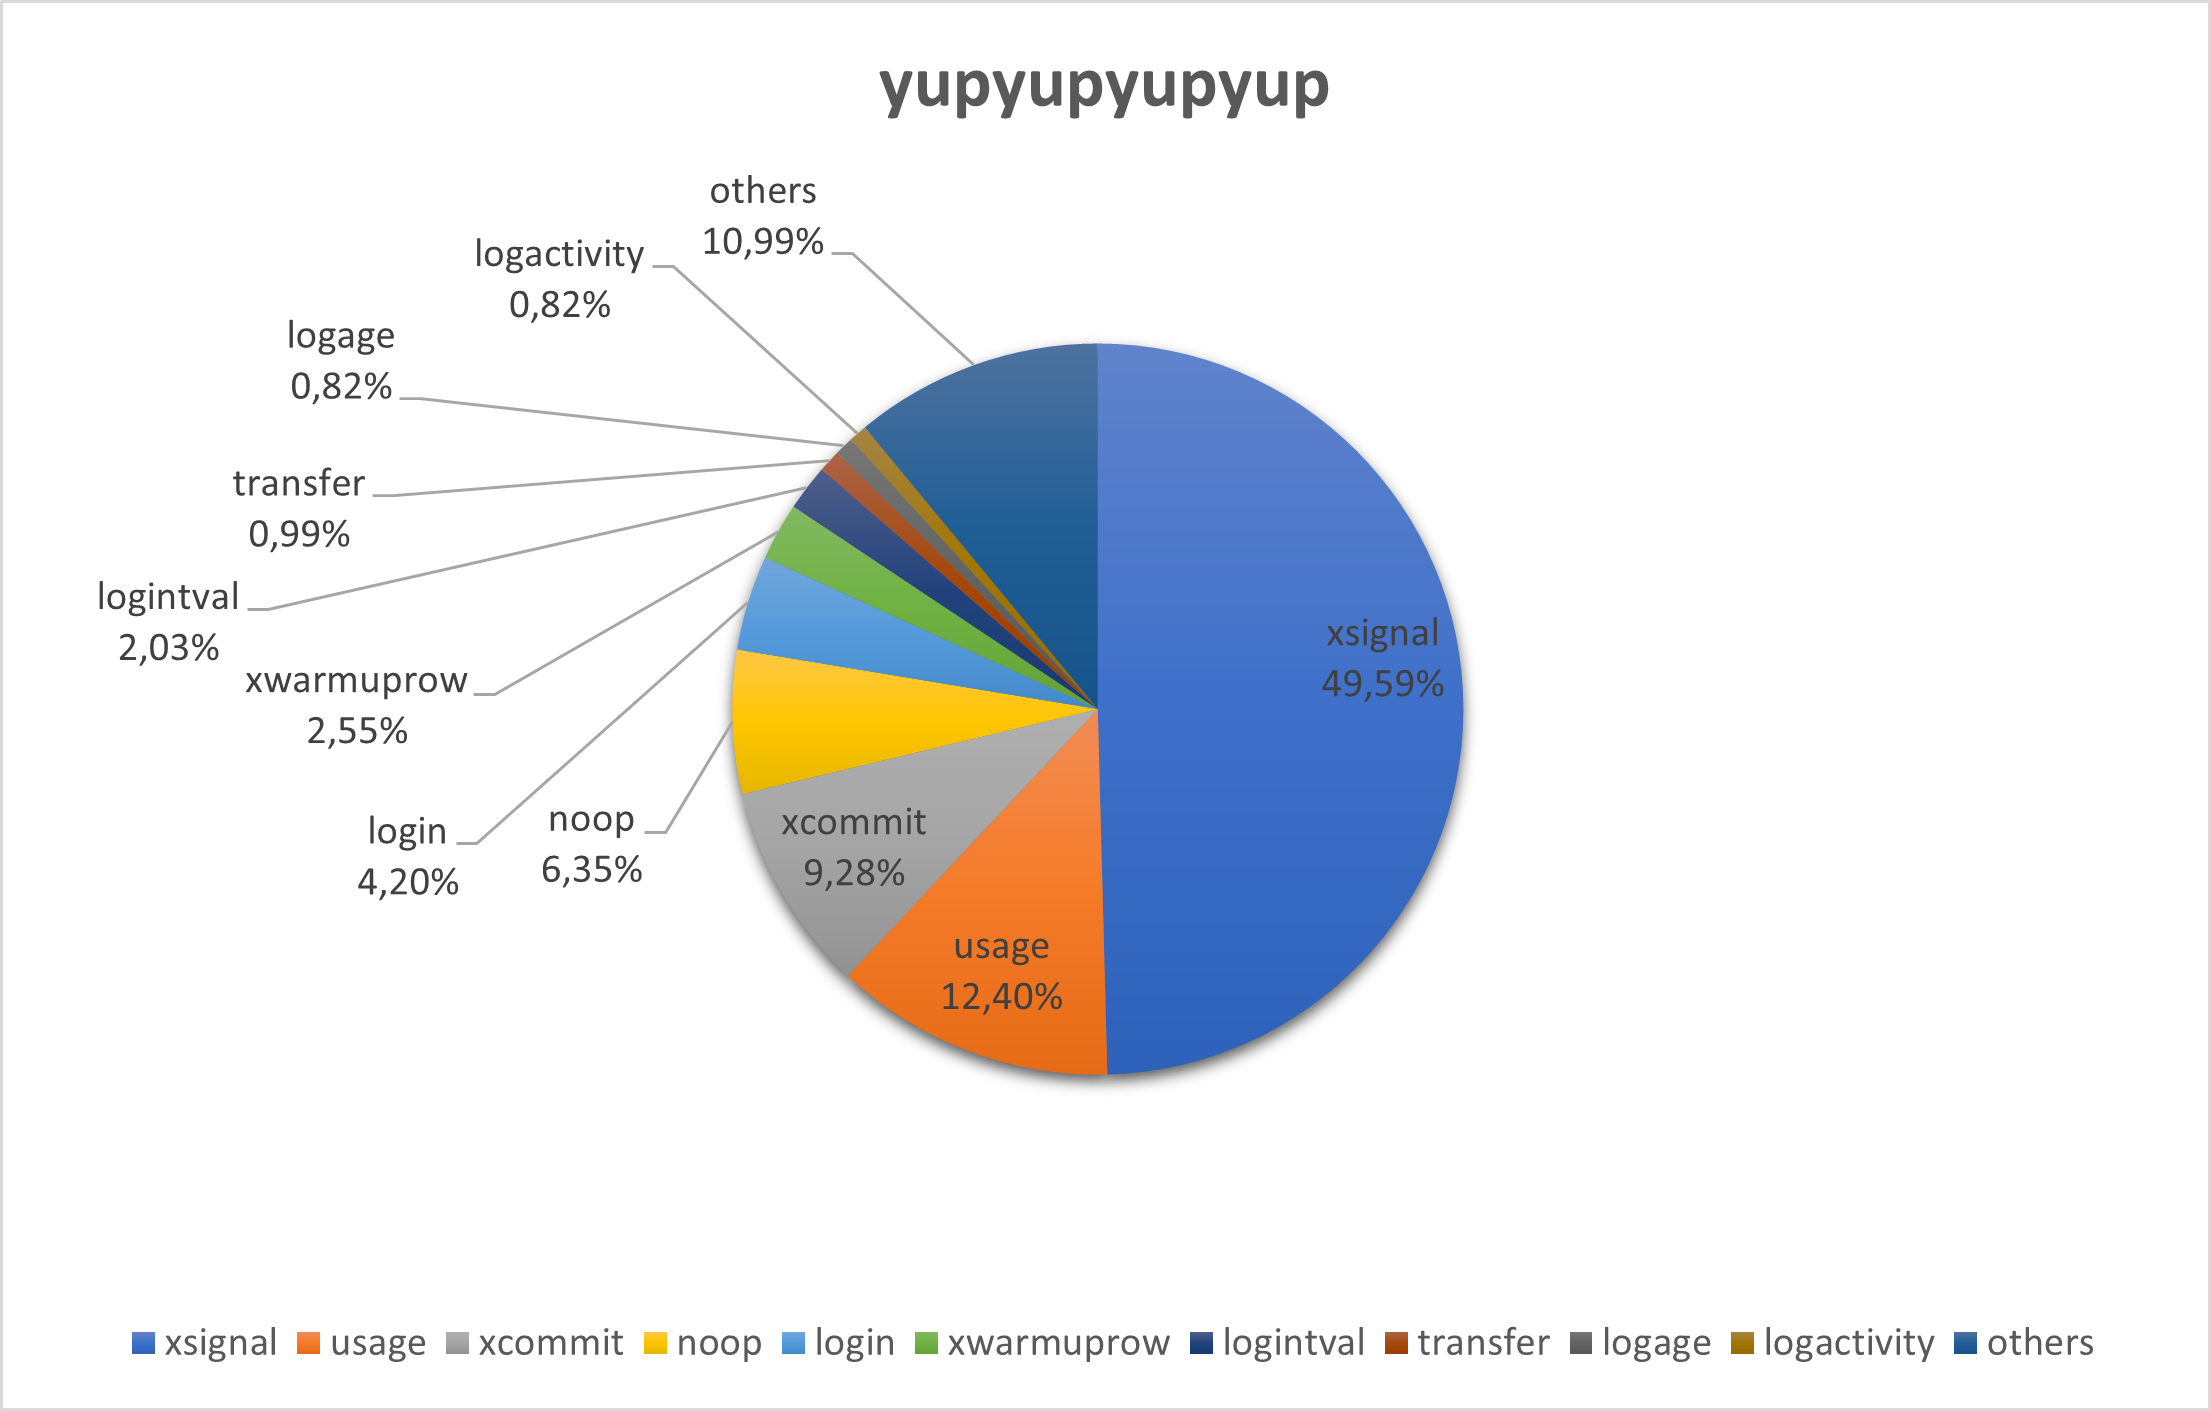
\includegraphics[width=1\textwidth]{graphs/torta_azioni.png}
    \caption{Rappresenta la distribuzione dei vari tipi di azioni, in \textbf{others} sono incluse tutte le azioni non presenti in top 10}
    \label{fig:actionsDistribution}
\end{figure}

In Figura \ref{fig:actionsDistribution} osserviamo come le tre azioni più utilizzate (\textit{xsignal}, \textit{usage} e \textit{xcommit}) facciano parte di quelle azioni non ritrovate nella lista dell'explorer (Tabella \ref{tab: unknown_actions} a Pagina \pageref{tab: unknown_actions}), dove la \textit{xsignal} ricopre quasi il 50\% delle azioni effettuate sul protocollo. Purtroppo non è stato possibile determinare con certezza la funzione di queste ultime, ma si suppone siano delle azioni proprie di EOS.IO relative alla gestione degli Smart Contract.
Un altro punto interessante di questa analisi consiste nell'aver individuato una buona presenza dell'azione \textit{noop} (no operation). Questa viene ripetuta un numero di volte considerevole (\textit{1.496.047}) se si considera che apparentemente non abbia alcun scopo, come dimostrato dal fatto che il campo \textit{data} del JSON che la caratterizza è completamente vuoto. Ciononostante, è importante notare che l'esecuzione di questa operazioni consumi comunque risorse, anche se non ha nessun effetto concreto.

\begin{figure}[h!]
    \centering
    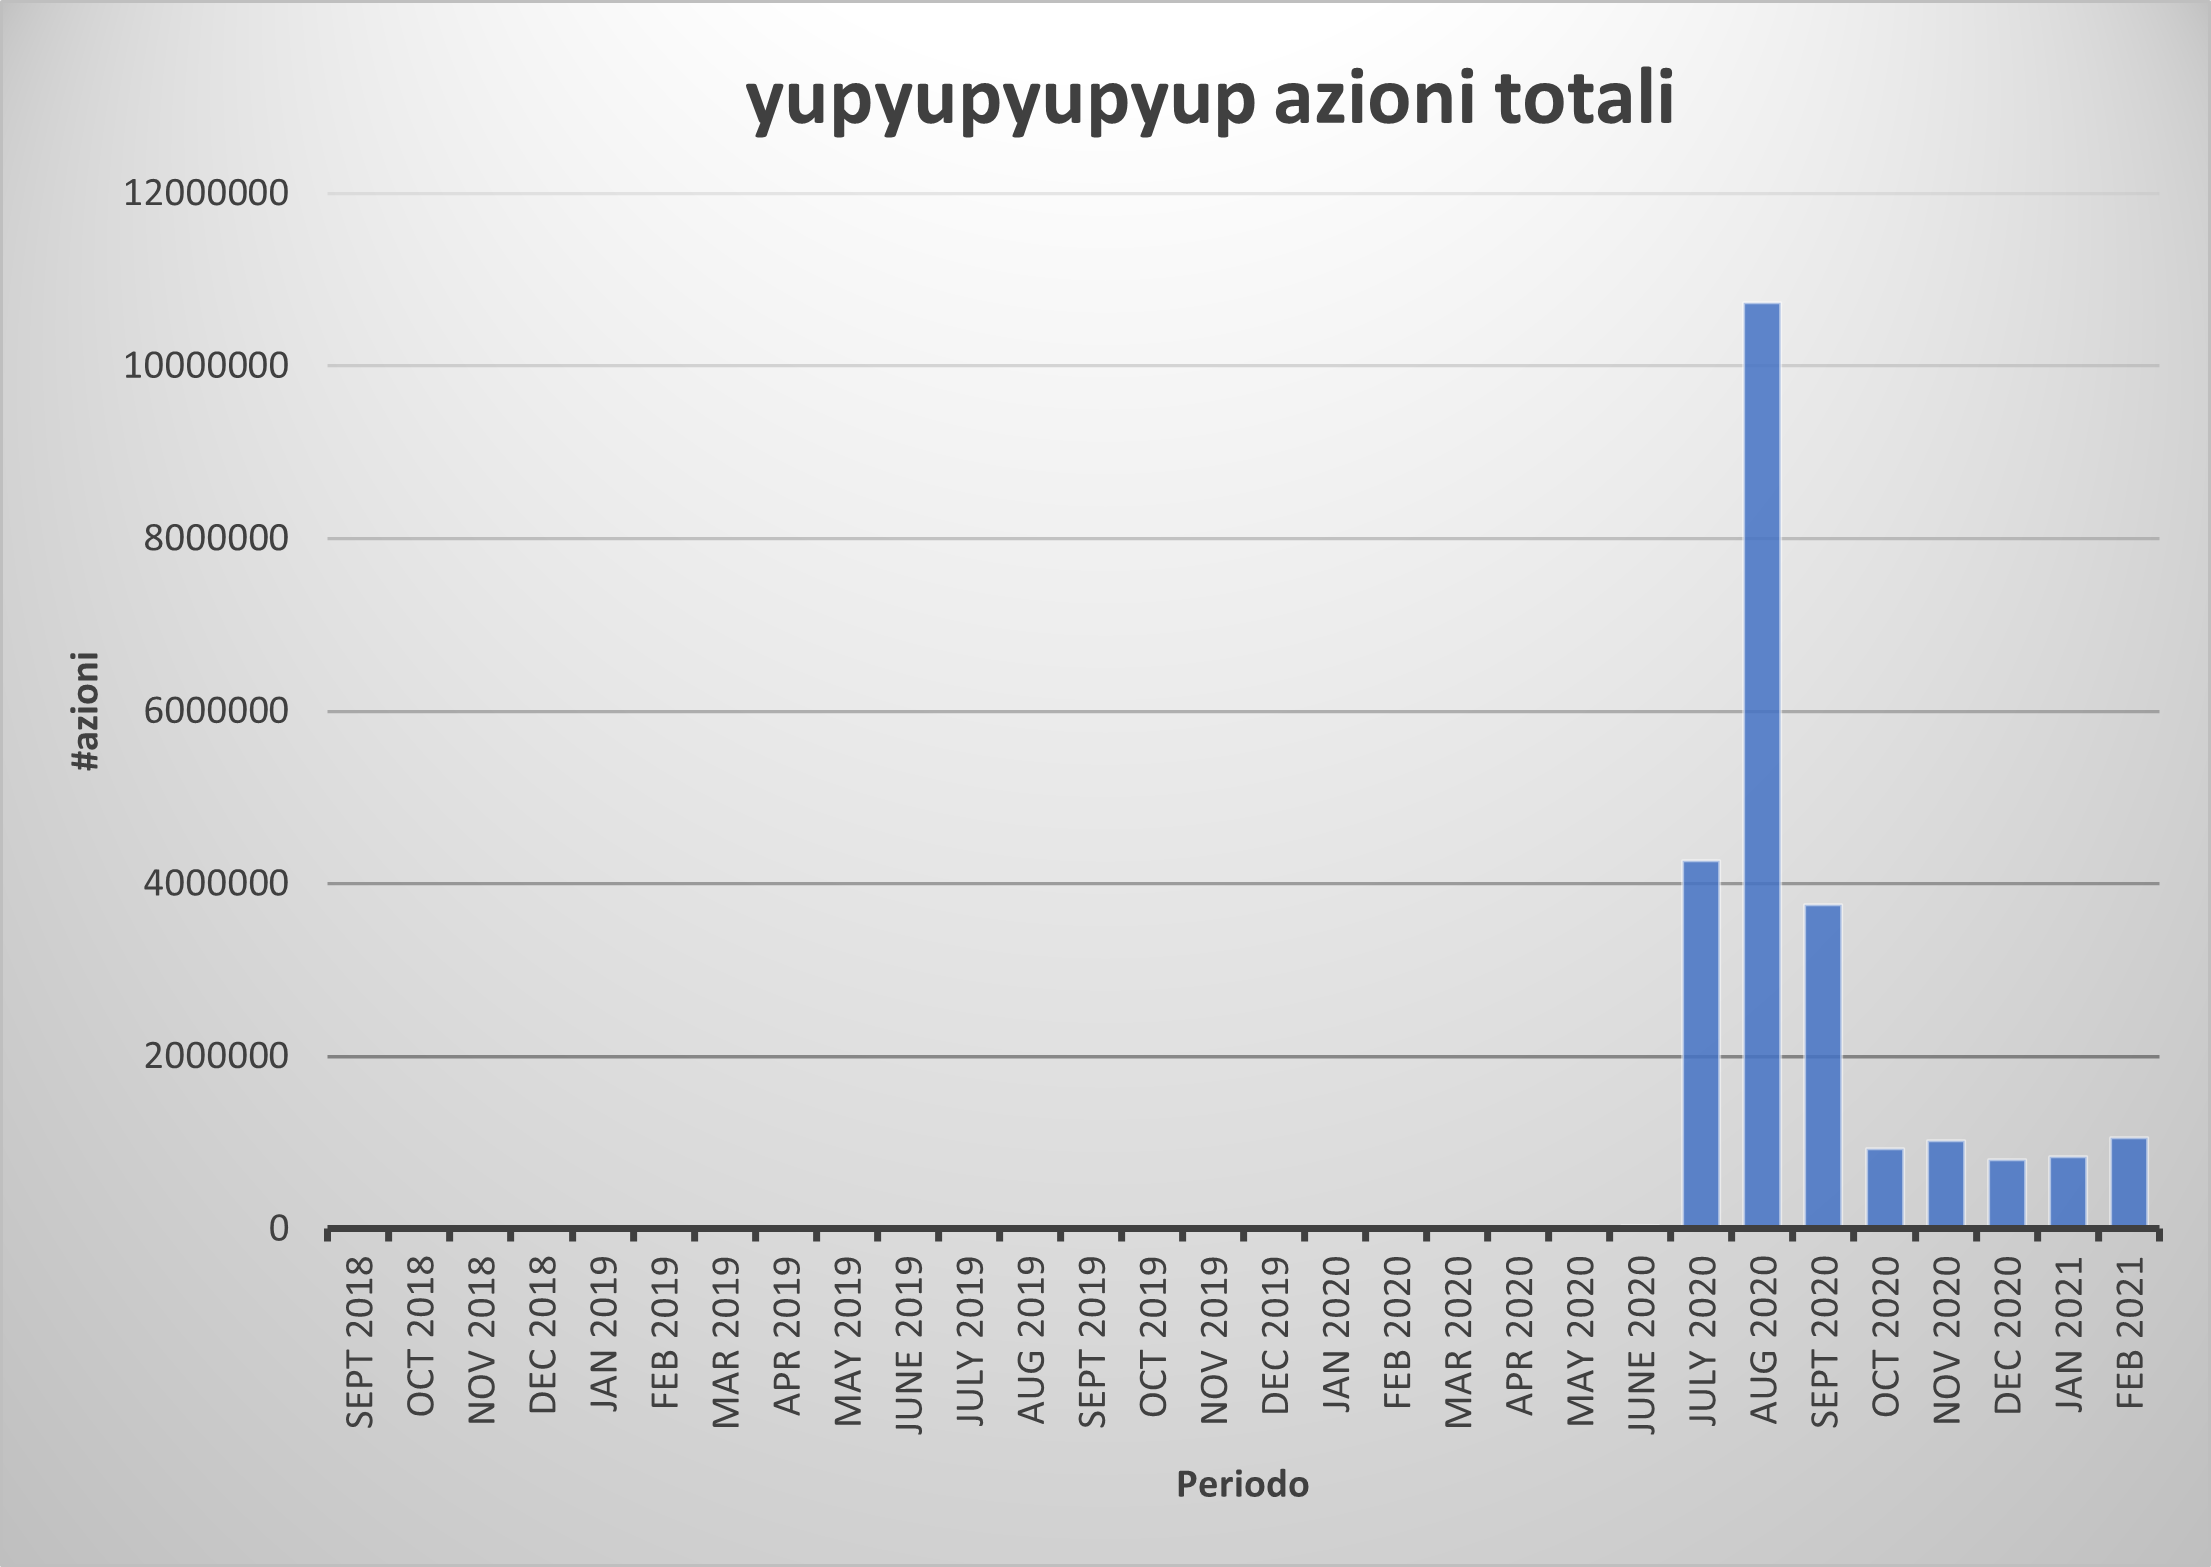
\includegraphics[width=1\textwidth]{graphs/mensile_azioni.png}
    \caption{Rappresenta la distribuzione delle azioni su base mensile, senza distinzione dei tipi, in modo da individuare particolari picchi di attività.}
    \label{fig:actionsMensile}
\end{figure}

In Figura \ref{fig:actionsMensile} possiamo constatare come l'attività del protocollo fino al mese di Giugno 2020 sia pressoché insignificante se paragonata ai mesi successivi. Abbiamo un particolare picco di attività nel periodo di Agosto 2020 ed è molto interessante come questo sia causato quasi esclusivamente da sole 4 azioni: \textbf{xsignal (6.805.319)}, \textbf{usage (1.701.330)}, \textbf{xcommit (1.293.877)} e \textbf{xwarmuprow (330.829)}. Queste costituiscono infatti più del 94\% dell'attività in quel mese. Purtroppo non è individuato alcun motivo che possa motivare un tale incremento in attività. E' tuttavia possibile che la ragione sia legata alla preparazione al passaggio tra la fase Beta di Yup e quella finale, entrata in funzione il \textit{6 Ottobre 2020}. 

\section{Utenza}
I dati relativi agli utenti Yup sono stati reperiti in due modalità: conteggiando il numero di \textbf{createacct} sullo smart contract e scaricando il JSON contente tutti gli utenti dalle API ufficiali.
Tuttavia, il numero di utenti ottenuti tramite API ufficiali non coincide con il numero di createacct, il che ci porta a pensare che alcuni utenti siano stati registrati senza l'interazione con il protocollo.
Per chiarezza, definiamo \textit{Creati} gli account per i quali esiste un'azione createacct, e \textit{non-Creati} gli altri account ottenuti dalle API, ma per i quali non esiste l'azione createacct.
%Come vedremo a breve il numero di account presenti nel JSON è notevolmente superiore al numero di createacct, ciò significa che esistono account non generati tramite l'interazione con il protocollo.

In Tabella \ref{table:usersClassification} mostriamo il numero degli utenti reperiti.

\begin{table}[h!]
\centering
\begin{tabular}{ |c|c|c|c|c|c| }
 \hline
 \textbf{Totale} & non-Creati & Creati & Mirror & non-Mirror\\
 \hline
 \textbf{16.484} & 5.439 & 11.045 & 7.607 & 3.438\\
 \hline
\end{tabular}
\caption{Classificazione dei tipi di account a Febbraio 2021}
\label{table:usersClassification}
\end{table}

La tabella mostra che il numero di account non-creati è circa la metà di quelli creati, e tra quelli creati una larga parte sono account mirror.
Poco meno di un terzo degli account creati sono non-Mirror e di questi meno della metà (un decimo del totale) hanno collegato il loro account Twitter all'account Yup.
In totale ci sono 7.607 Mirror e 8.877 non-Mirror.

In Figura \ref{fig:usersClassification2}, considerando solo gli account non-Mirror, proponiamo un confronto tra la distribuzione di account linkati a Twitter e non (registrati tramite e-mail o WalletConnect).

\begin{figure}[t]
    \centering
    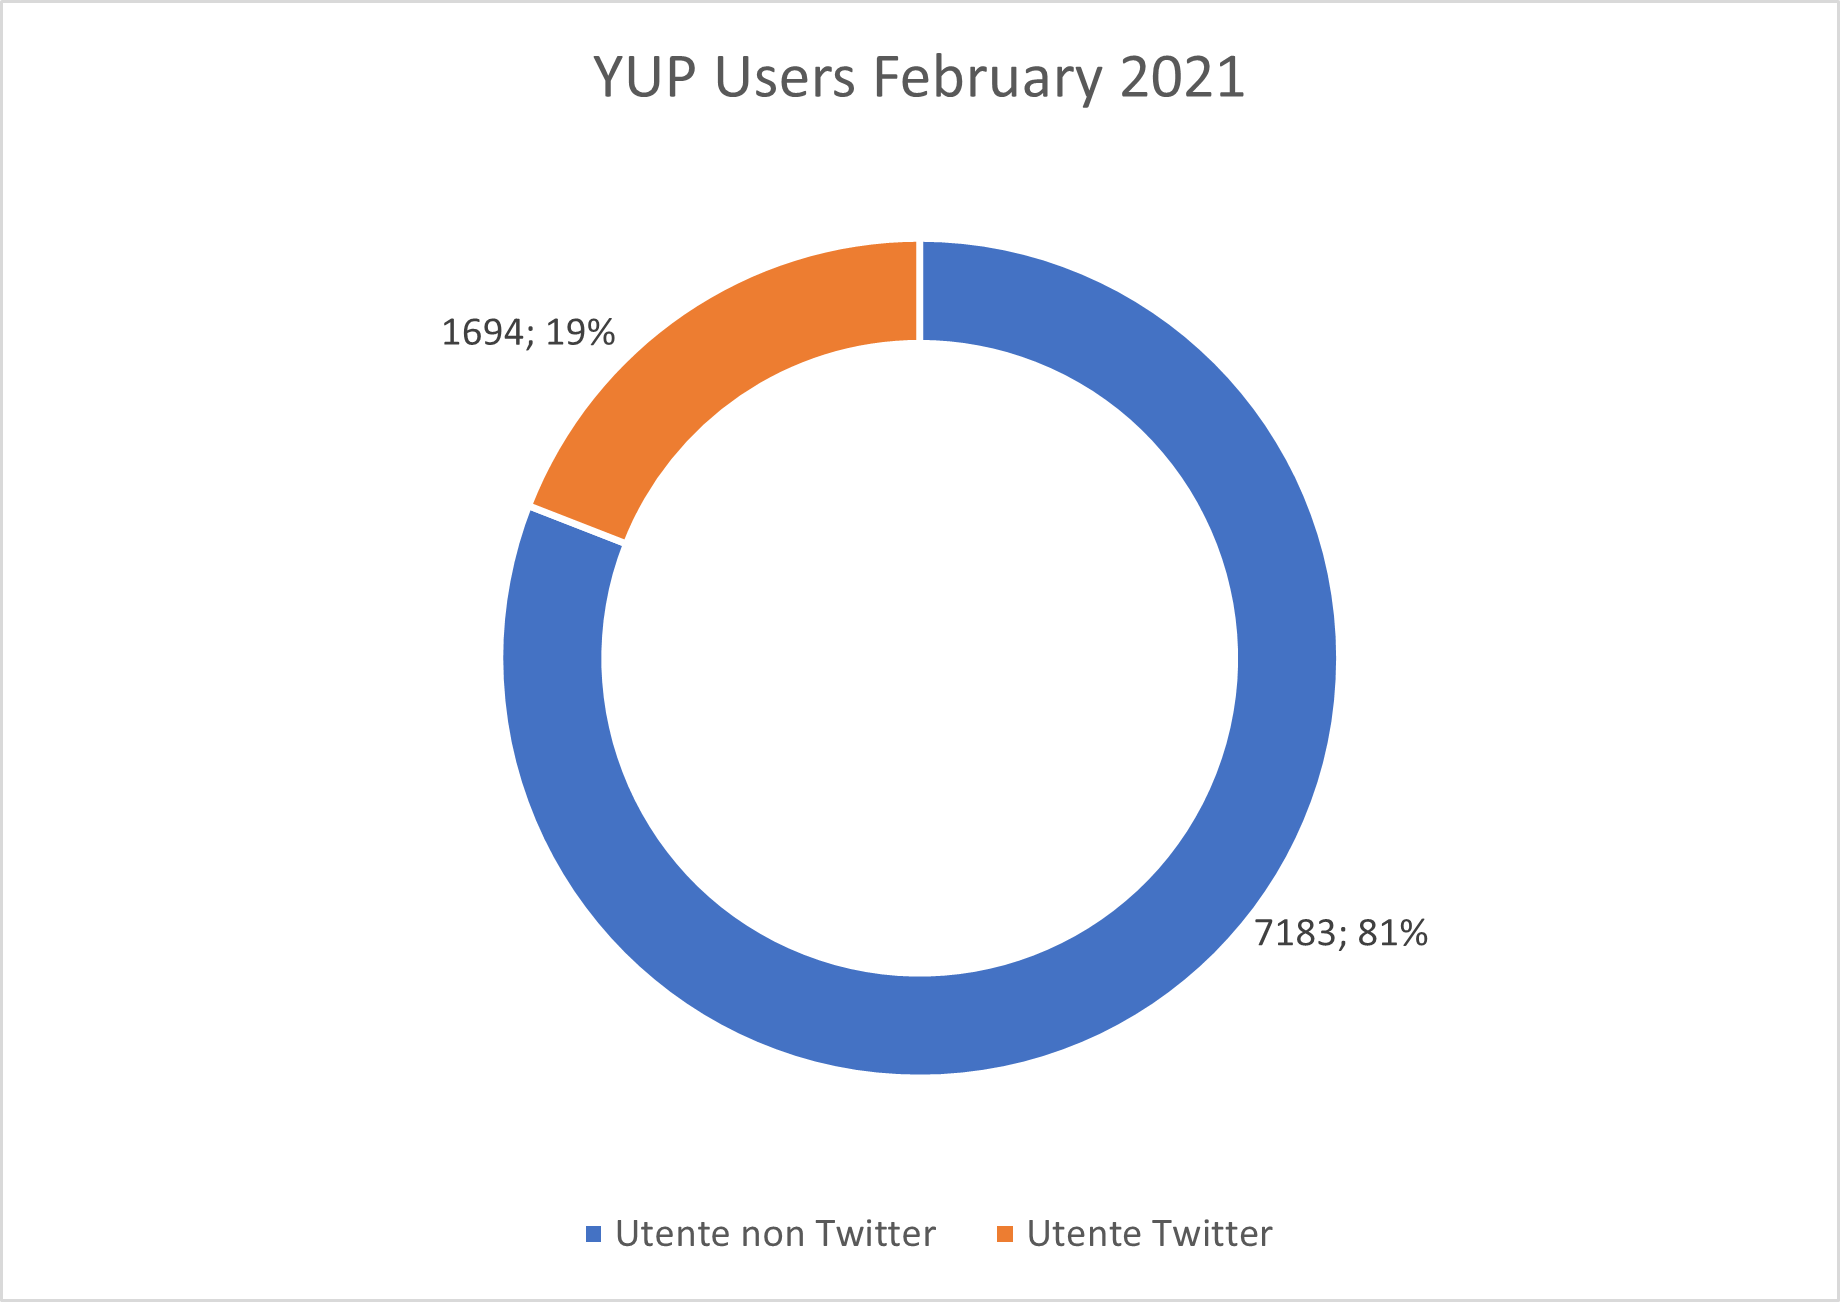
\includegraphics[width=0.8\textwidth]{graphs/users_feb.png}
    \caption{Tipi di utenti Febbraio 2021}
    \label{fig:usersClassification2}
\end{figure}

Dalla Figura è facile accorgersi come, almeno al momento, la maggior parte degli utenti Yup non si sia registrata alla piattaforma mediante il proprio account Twitter oppure semplicemente non abbia effettuato il linking una volta registrato tramite Email o Wallet Connect.
Questo potrebbe essere legato al fatto che la piattaforma non è ancora ben conosciuta al mondo social, nonostante la sua integrazione, o che gli utenti a cui si rivolge sono perlopiù legati o familiari con il mondo delle criptovalute.


Essendo presente, nel caso di alcuni account, questo collegamento tra Yup e Twitter, siamo andati a vedere che relazione ci fosse tra le relazioni di follow tra gli utenti sulle due piattaforme. Sono stati tenuti in considerazione solo i follower di account Yup collegati a Twitter, altrimenti non sarebbe stato possibile effettuare la verifica. Mostriamo in Figura \ref{fig:followersComparison} le relazioni di follow presenti solo su Yup (in blu) e quelle presenti sia su Yup che su Twitter (in arancione).

\begin{figure}[t]
    \centering
    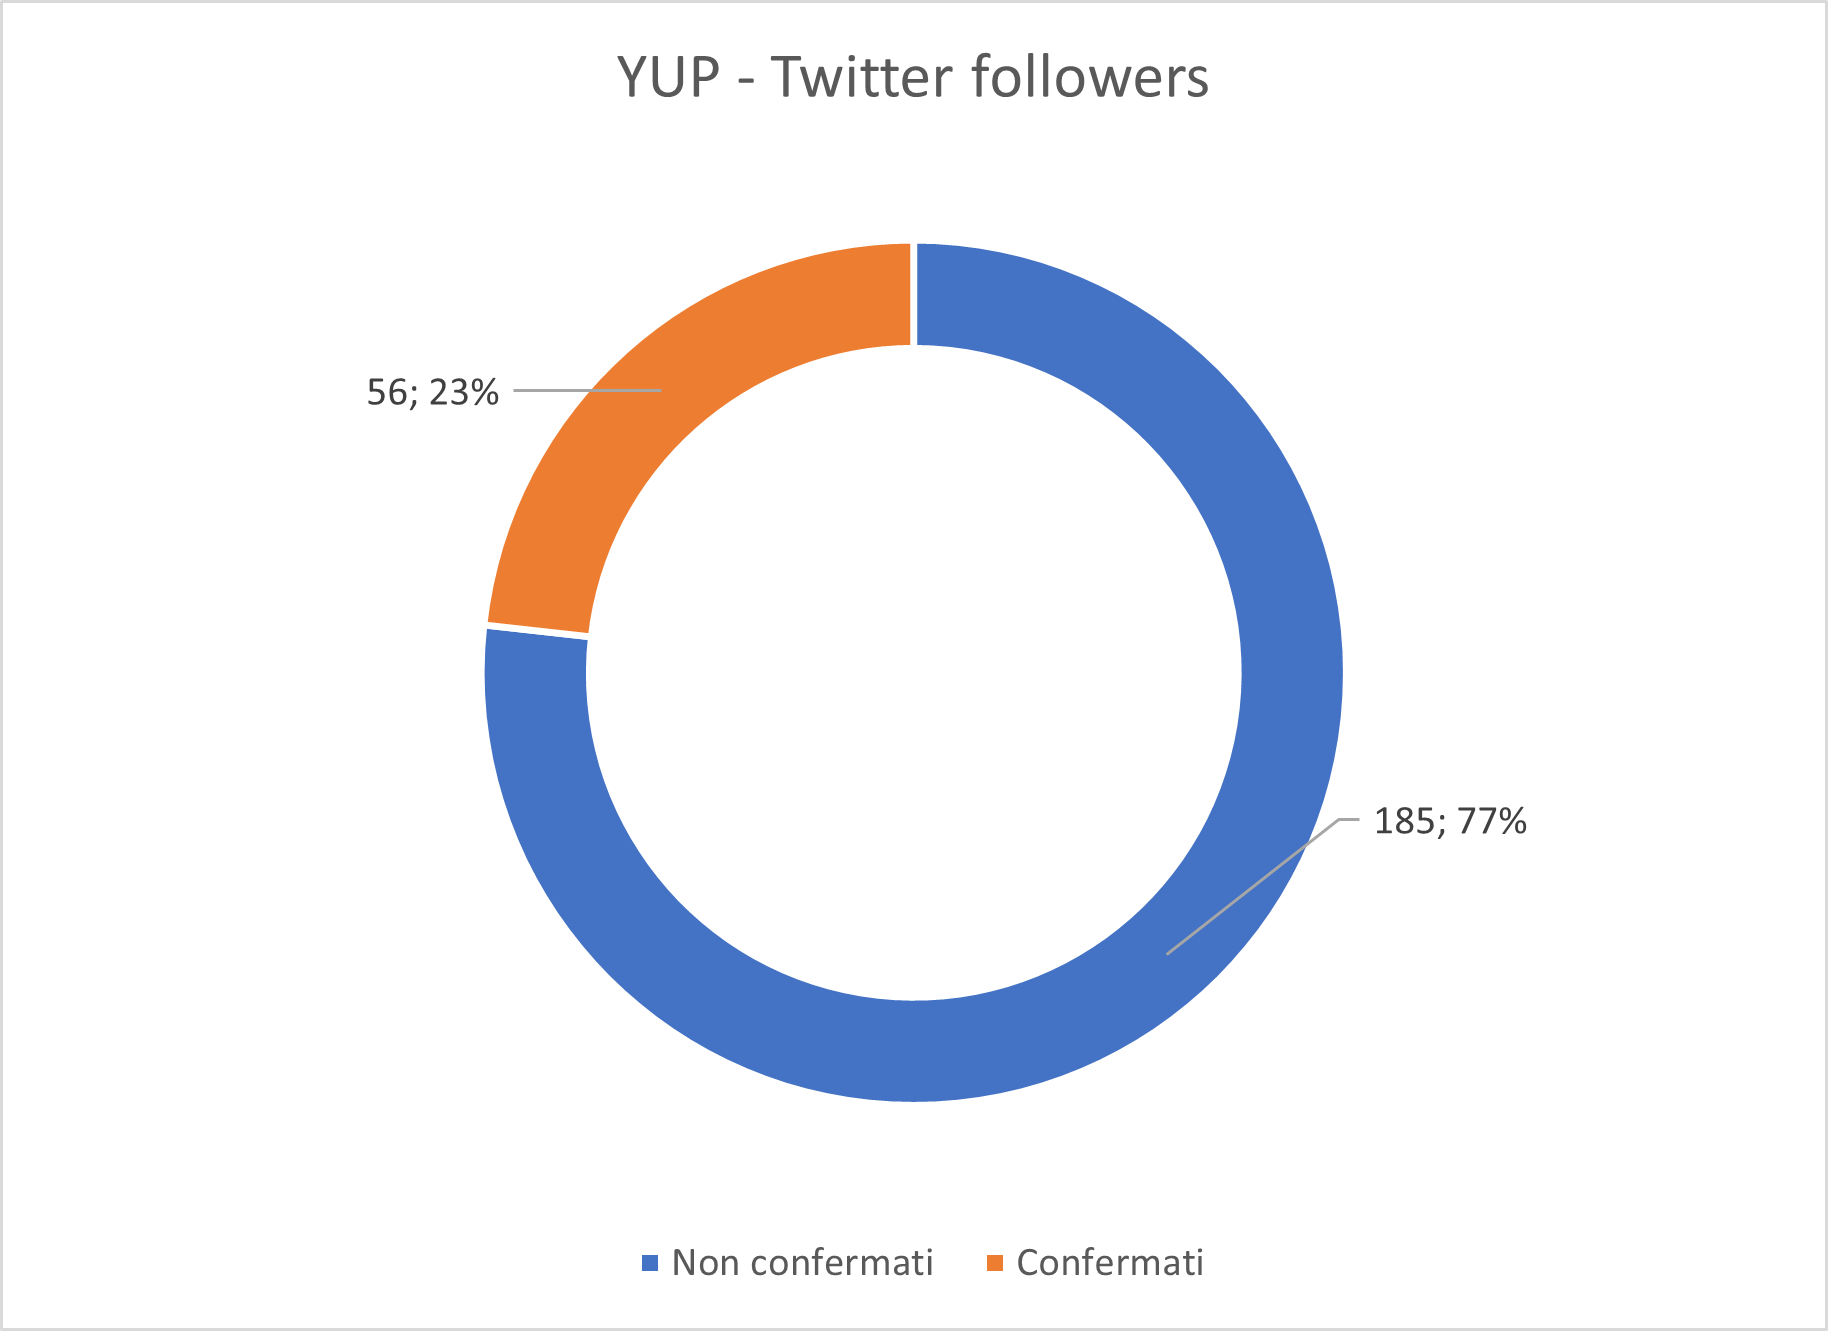
\includegraphics[width=0.8\textwidth]{graphs/followers.png}
    \caption{Follower confermati, segue su Yup e segue anche su Twitter, e quelli non confermati, non segue su Twitter.}
    \label{fig:followersComparison}
\end{figure}

Questa analisi ci permette di affermare che, almeno tra gli utenti Yup con un account Twitter collegato, la funzionalità di following sulla piattaforma viene raramente utilizzata, infatti troviamo solo 241 follow espressi da su quasi 1.700 utenti. Oltretutto in oltre 3/4 dei casi, l'utente che segue lo fa solamente su Yup.
Questi risultato mette in luce il fatto che il follow su Yup non tende ad avere funzioni sociali come su Twitter.

\subsection{Createacct}
Anche per le azioni di creazione account (createacct) è stata effettuata un'analisi temporale su base mensile. In questo modo ci è possibile apprendere quali siano stati i mesi chiave che hanno visto un maggiore di utenti registrati sulla piattaforma. Mostriamo in Figura \ref{fig:createacctMensile_conmirr} e \ref{fig:createacctMensile_nomirr} il numero di createacct per mese, rispettivamente includendo ed escludendo account Mirror.

\begin{figure}[t]
    \centering
    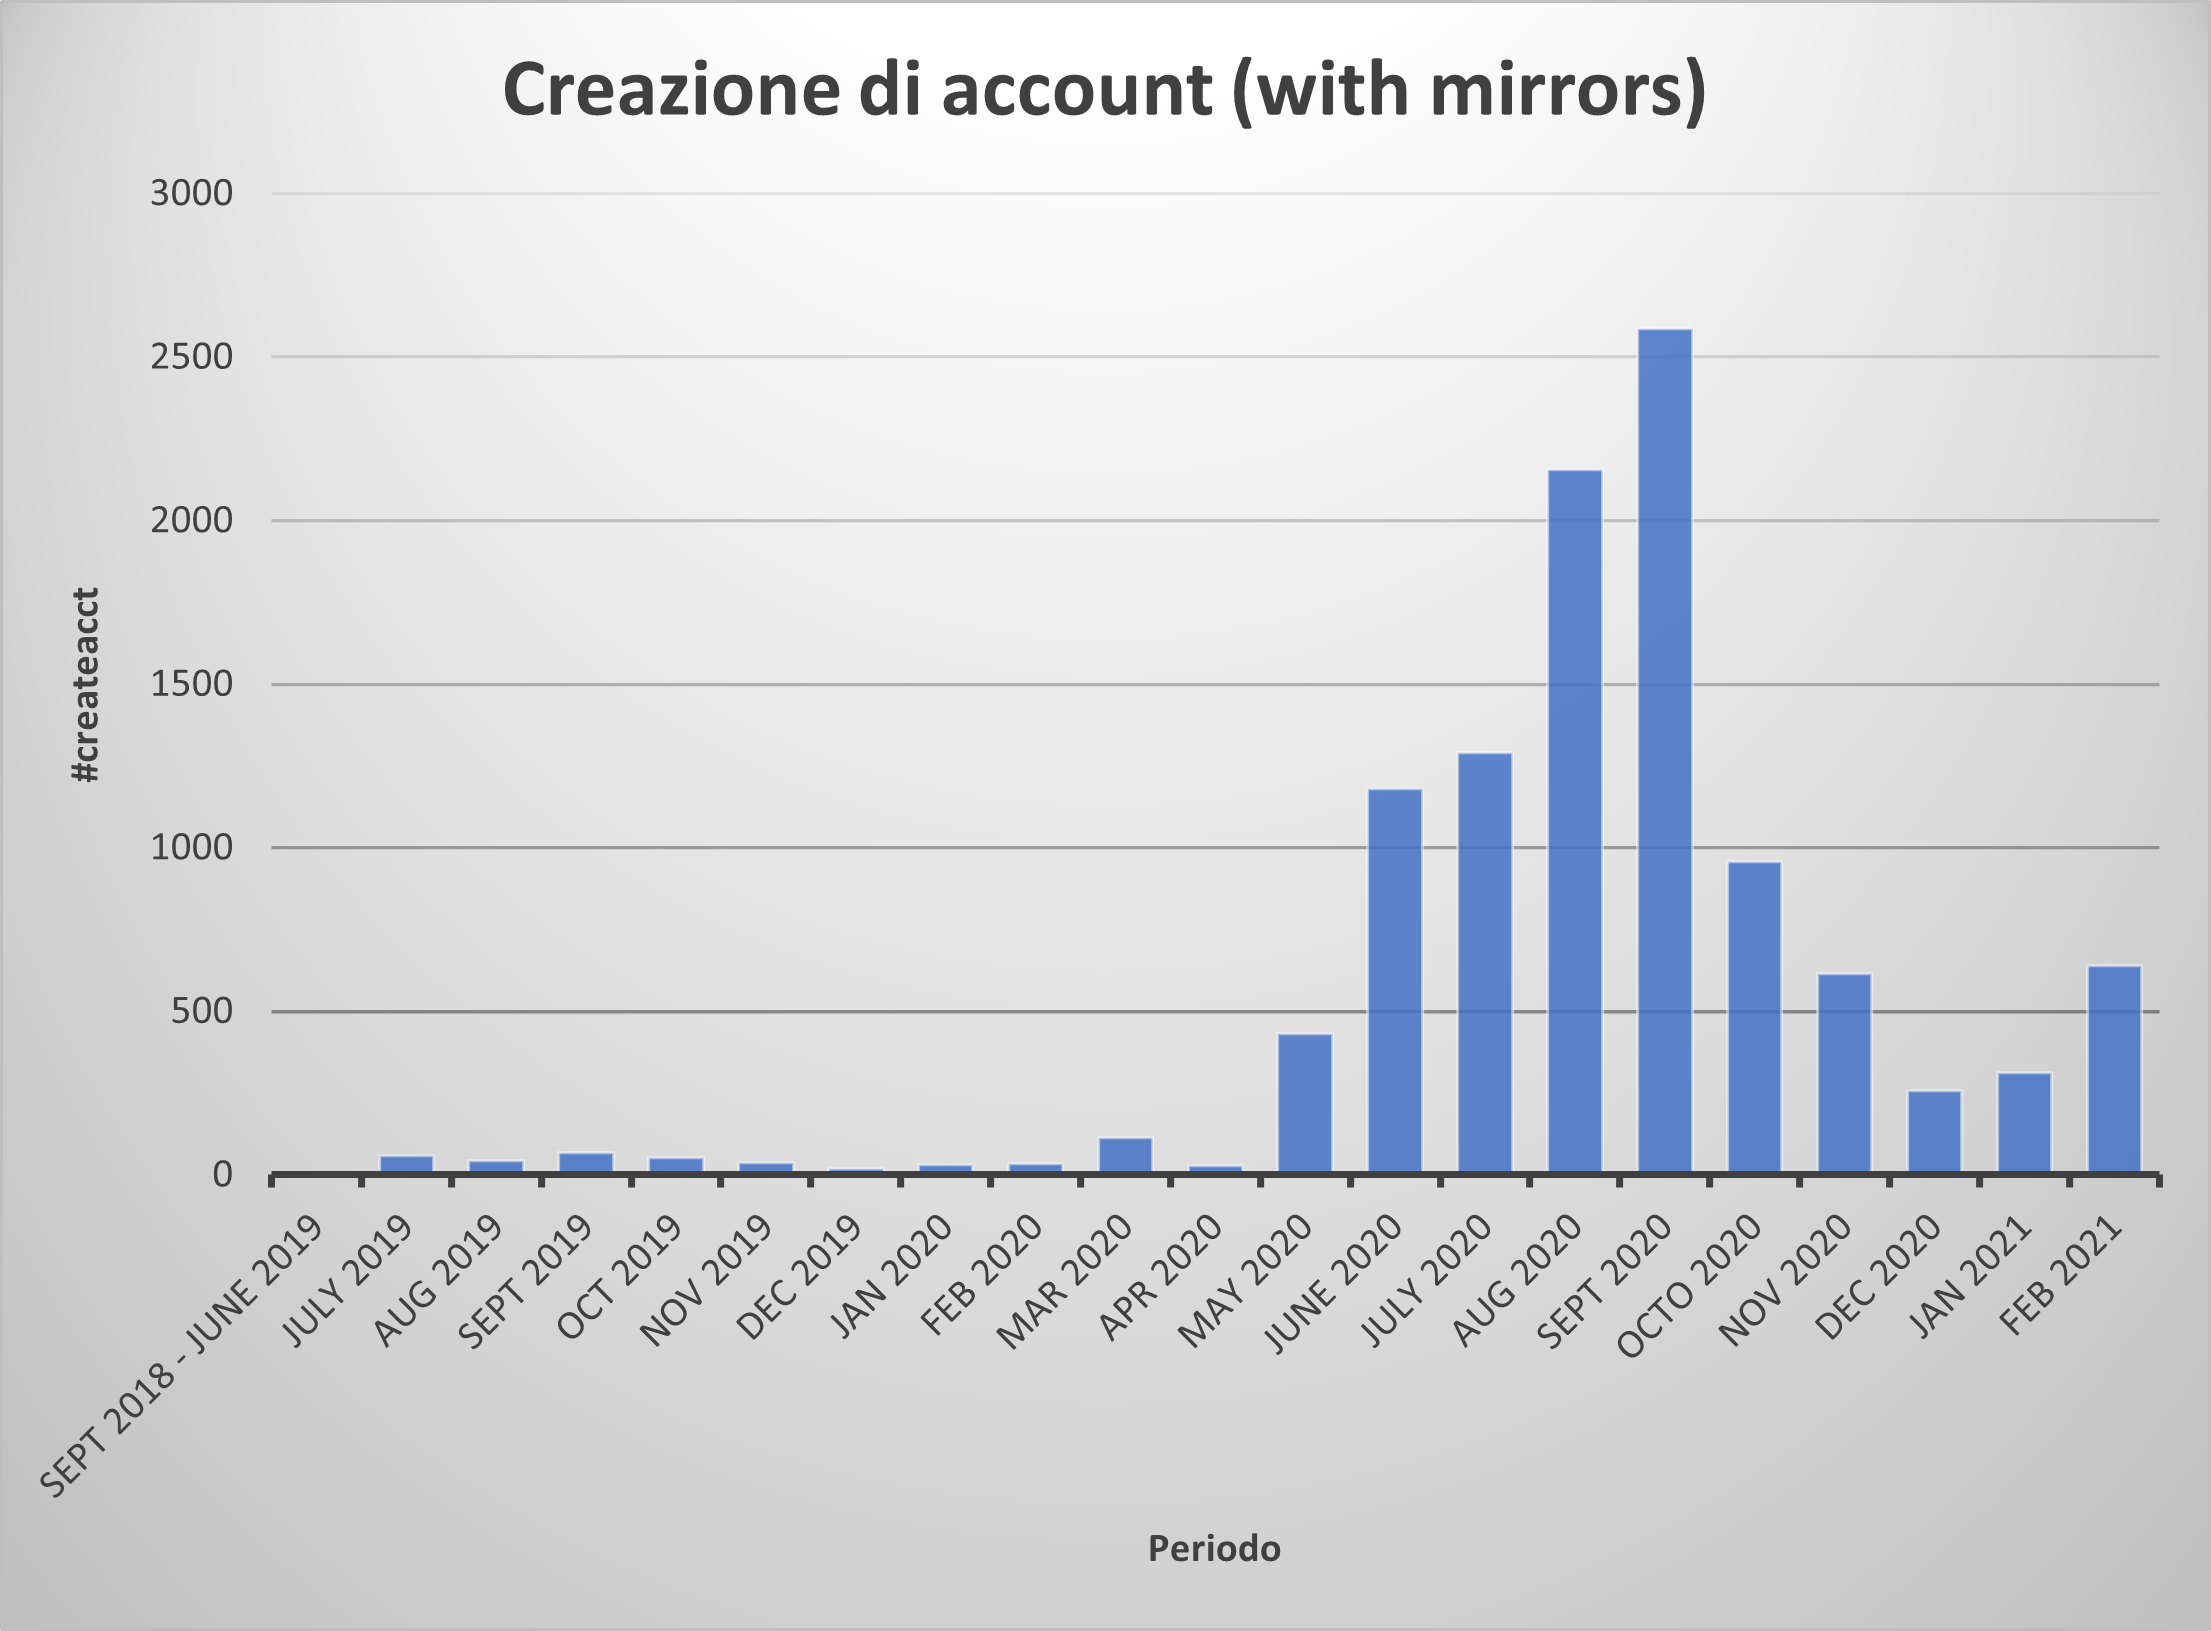
\includegraphics[width=.7\textwidth]{graphs/createaccount.png}
    \caption{Distribuzione mensile delle \textbf{createacct} includendo account Mirror}
    \label{fig:createacctMensile_conmirr}
\end{figure}

\begin{figure}[t]
    \centering
    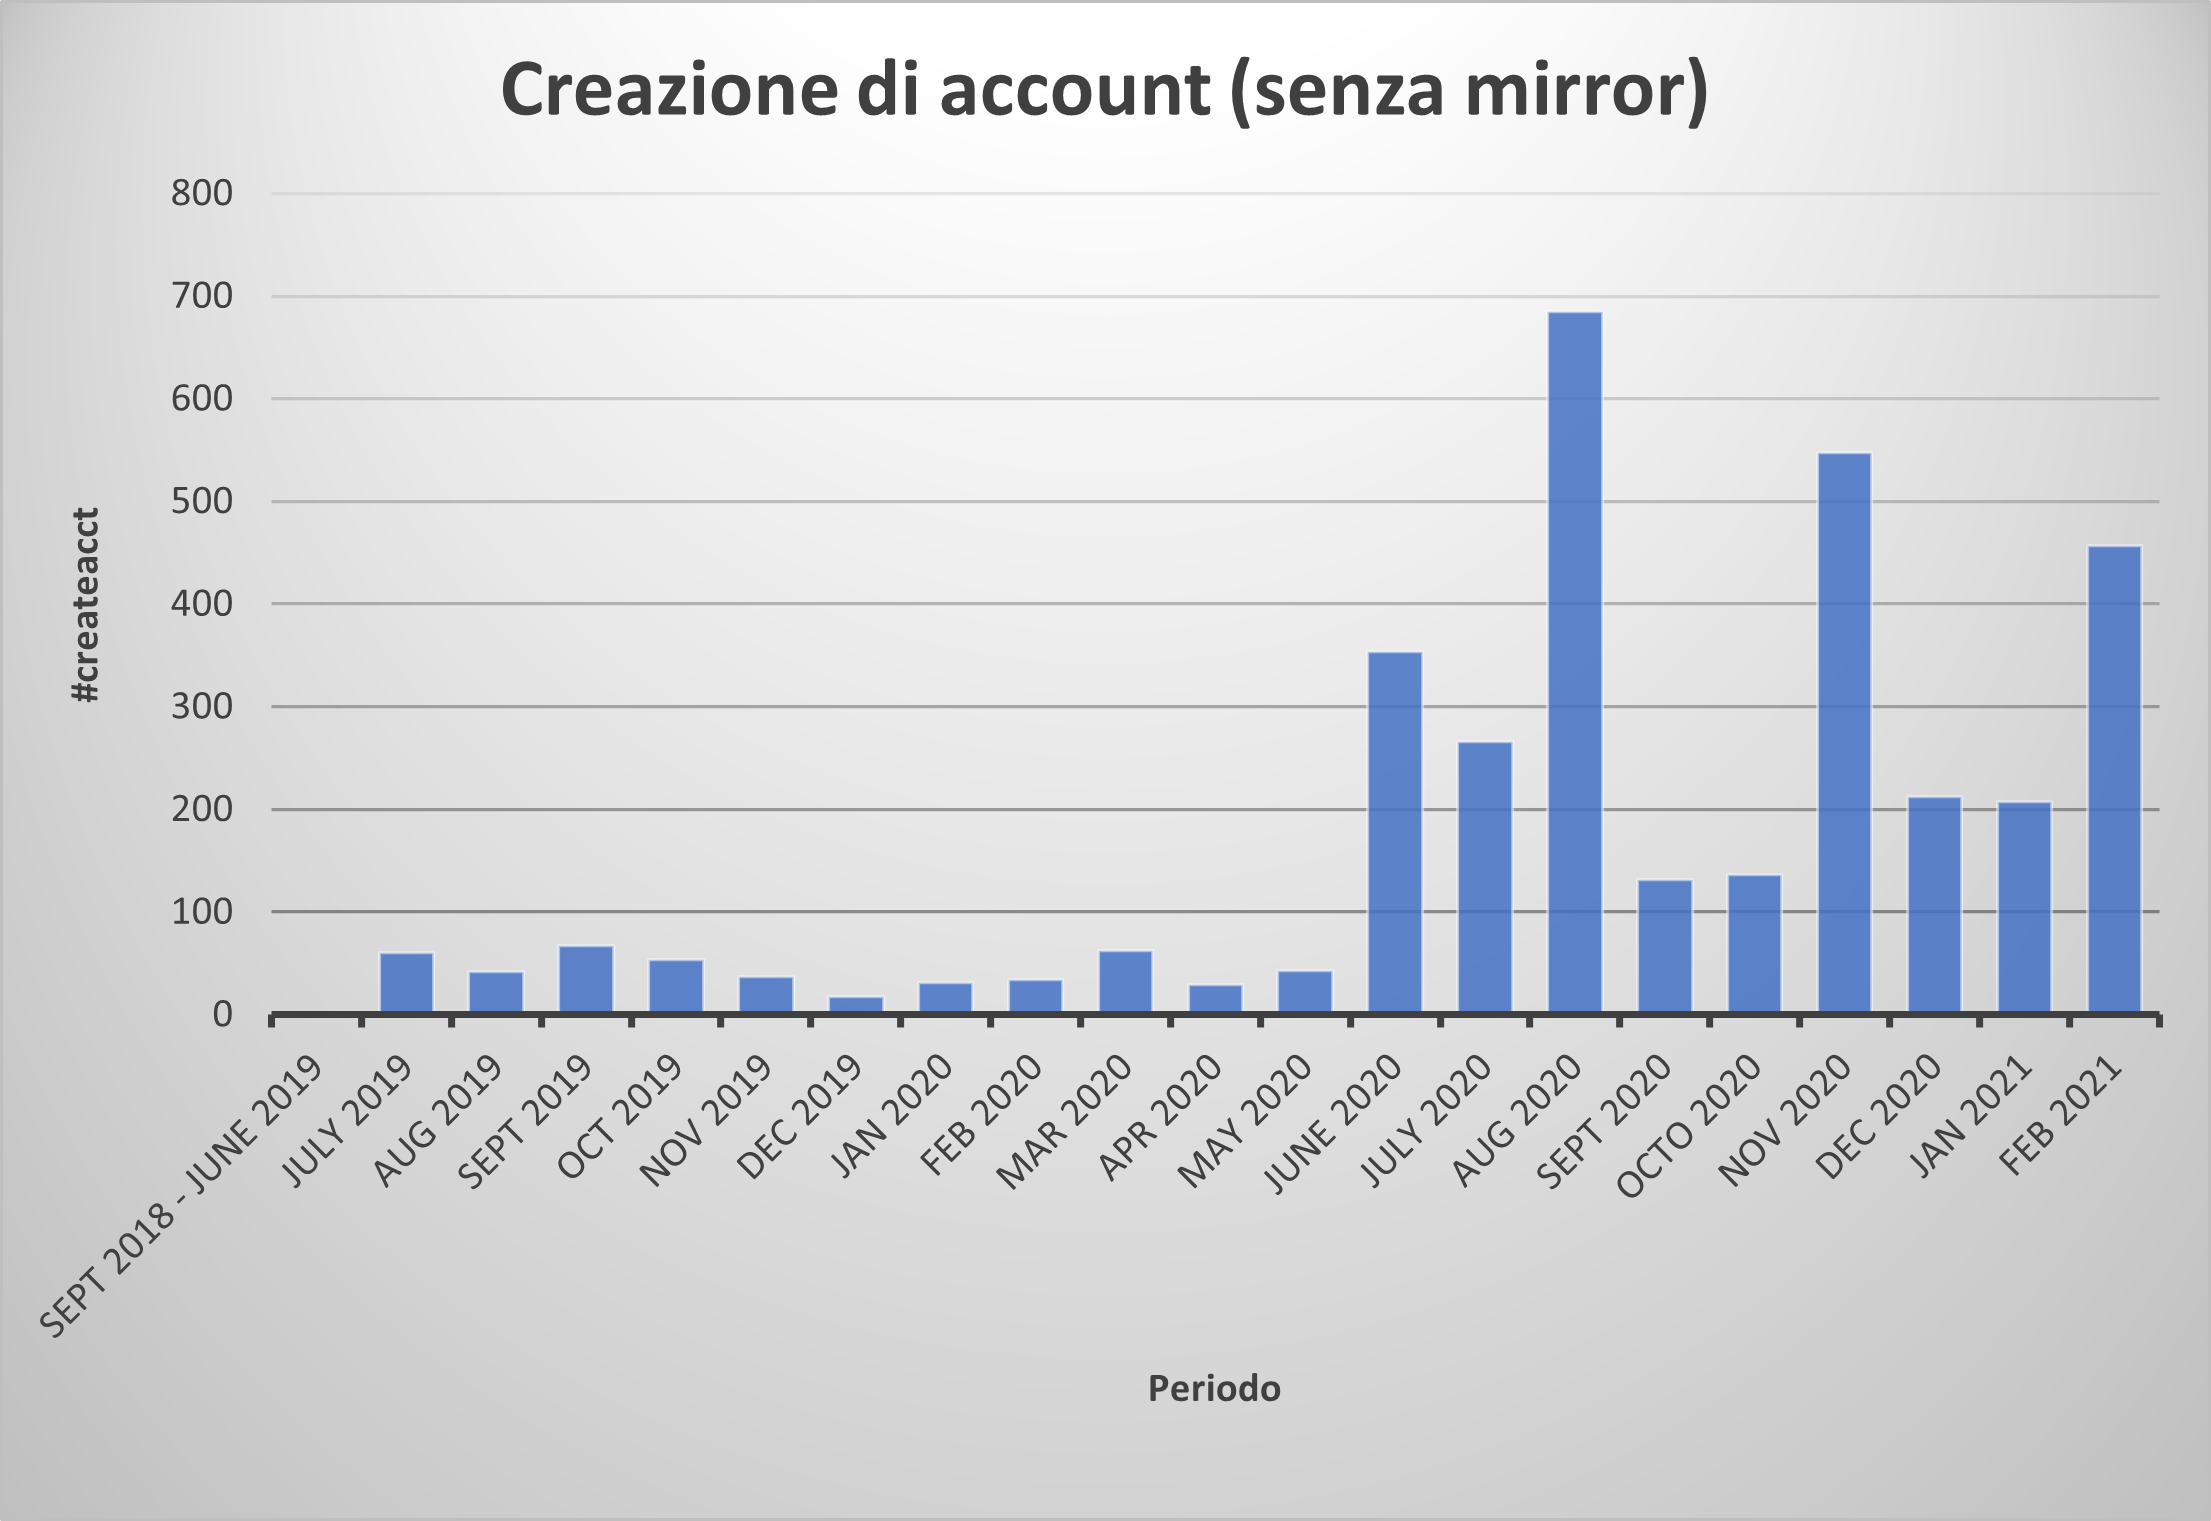
\includegraphics[width=.7\textwidth]{graphs/createaccount_nomirr.png}
    \caption{Distribuzione mensile delle \textbf{createacct} escludendo account Mirror}
    \label{fig:createacctMensile_nomirr}
\end{figure}

Non essendo a conoscenza dei criteri secondo cui vengono creati account Twitter Mirror su Yup è difficile avanzare ipotesi riguardo al grafico in Figura \ref{fig:createacctMensile_conmirr}. Possiamo tuttavia notare come fino ad Aprile 2020 la creazione di account, Mirror e non, fosse molto esigua se la paragoniamo a quella nei mesi successivi. Tra i mesi di Maggio 2020 e Novembre 2020 notiamo almeno 500 createacct al mese, con un picco di oltre 2.500 nuove creazioni nel solo mese di Settembre 2020, indice di come la piattaforma avesse iniziato a prendere piede grazie alle campagne pubblicitarie e all'inizio della fase beta aperta a tutti.
%Anche in questo caso il picco osservabile in entrambi i casi nei mesi di Agosto-Settembre potrebbe essere invece correlato al lancio della piattaforma in Ottobre.

Paragonando le Figure \ref{fig:createacctMensile_conmirr} e \ref{fig:createacctMensile_nomirr} notiamo che una larga porzione dei nuovi account sulla piattaforma proprio nel periodo Giugno 2020 - Novembre 2020 è formata da account Mirror.
Attribuiamo questo fenomeno a strategie utilizzate dai creatori di Yup per invogliare nuovi utenti ad unirsi alla piattaforma, mostrando quanto è possibile guadagnare.

\subsection{Utenti attivi-passivi}
Infine abbiamo analizzato, su base mensile, l'attività degli utenti facendo una classificazione in utenti attivi o passivi. Con \textbf{utenti attivi} indichiamo coloro che hanno effettuato un'azione di voto, follow, commento o modifica della biografia del proprio account in un dato periodo temporale, mentre con \textbf{utenti passivi} quelli che hanno effettuato solamente un'operazione di login. Un appunto che deve essere fatto è che quest'ultima classificazione è solo parziale poiché alcuni utenti potrebbero aver effettuato il login sulla piattaforma e successivamente non aver fatto nulla, quindi essere utenti passivi, ma tale azione non viene registrata sul protocollo perché il login è automatizzato con le credenziali salvate nella cache del browser. Mostriamo in Figura \ref{fig:attivi_conmirr} gli utenti attivi e passivi includendo gli account Mirror, e in Figura \ref{fig:attivi_nomirr} gli utenti attivi e passivi escludendo gli account Mirror.

\begin{figure}[t]
    \centering
    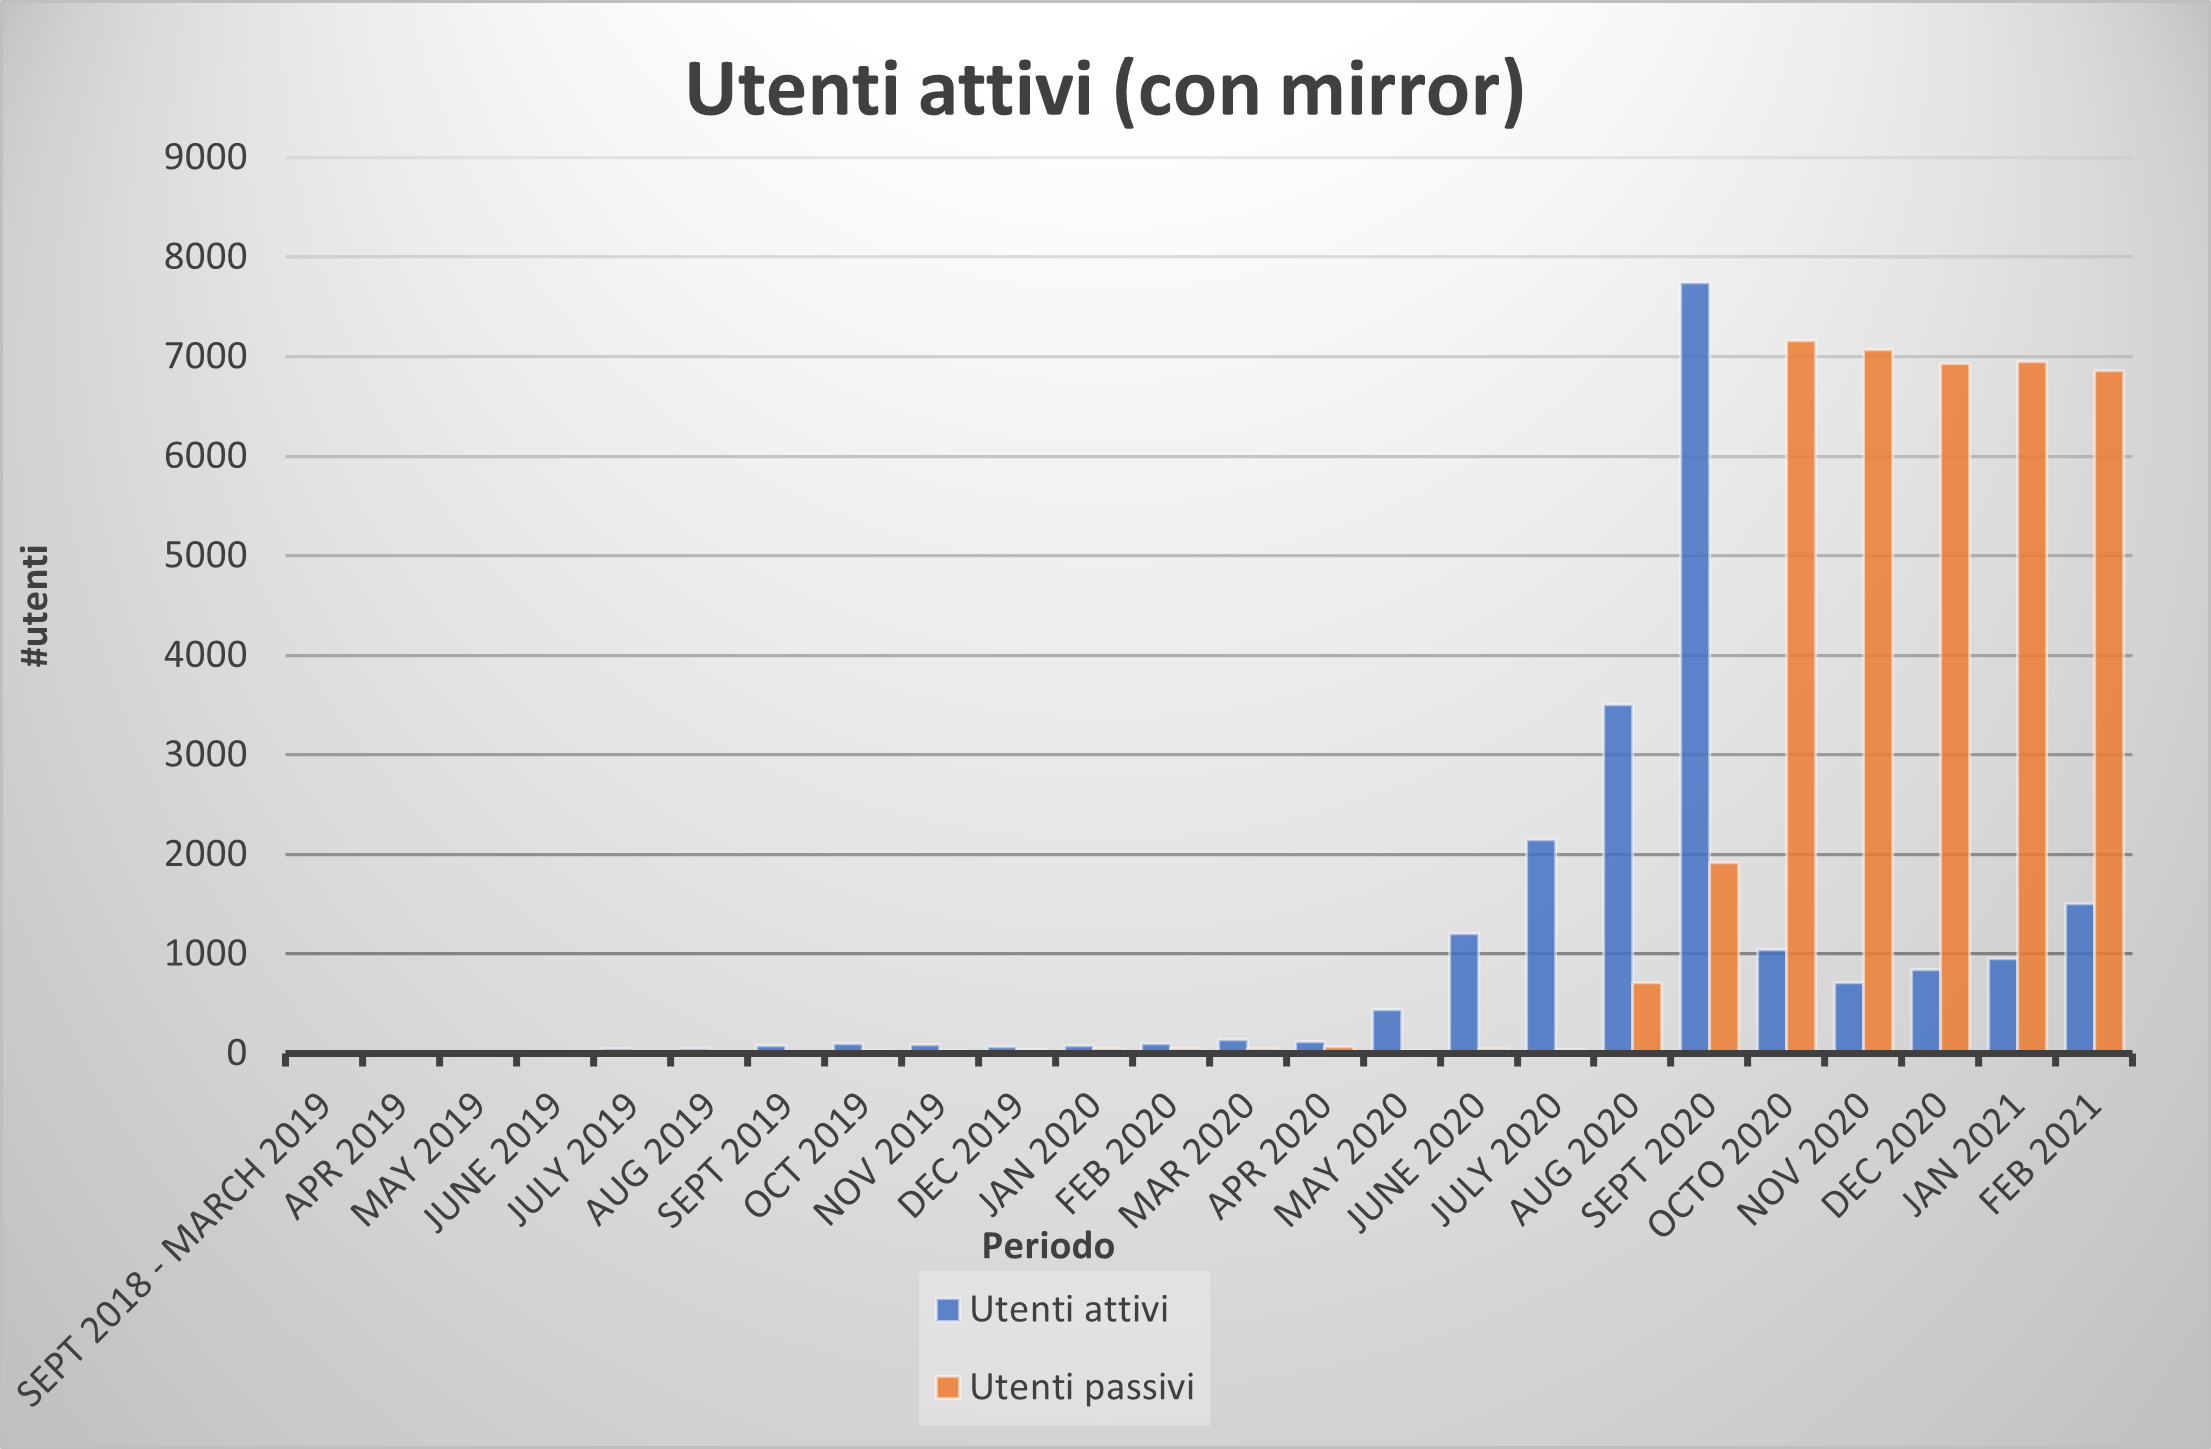
\includegraphics[width=0.7\textwidth]{graphs/utentiattivi.png}
    \caption{Utenti attivi-passivi su base mensile includendo account Mirror}
    \label{fig:attivi_conmirr}
\end{figure}

\begin{figure}[t]
    \centering
    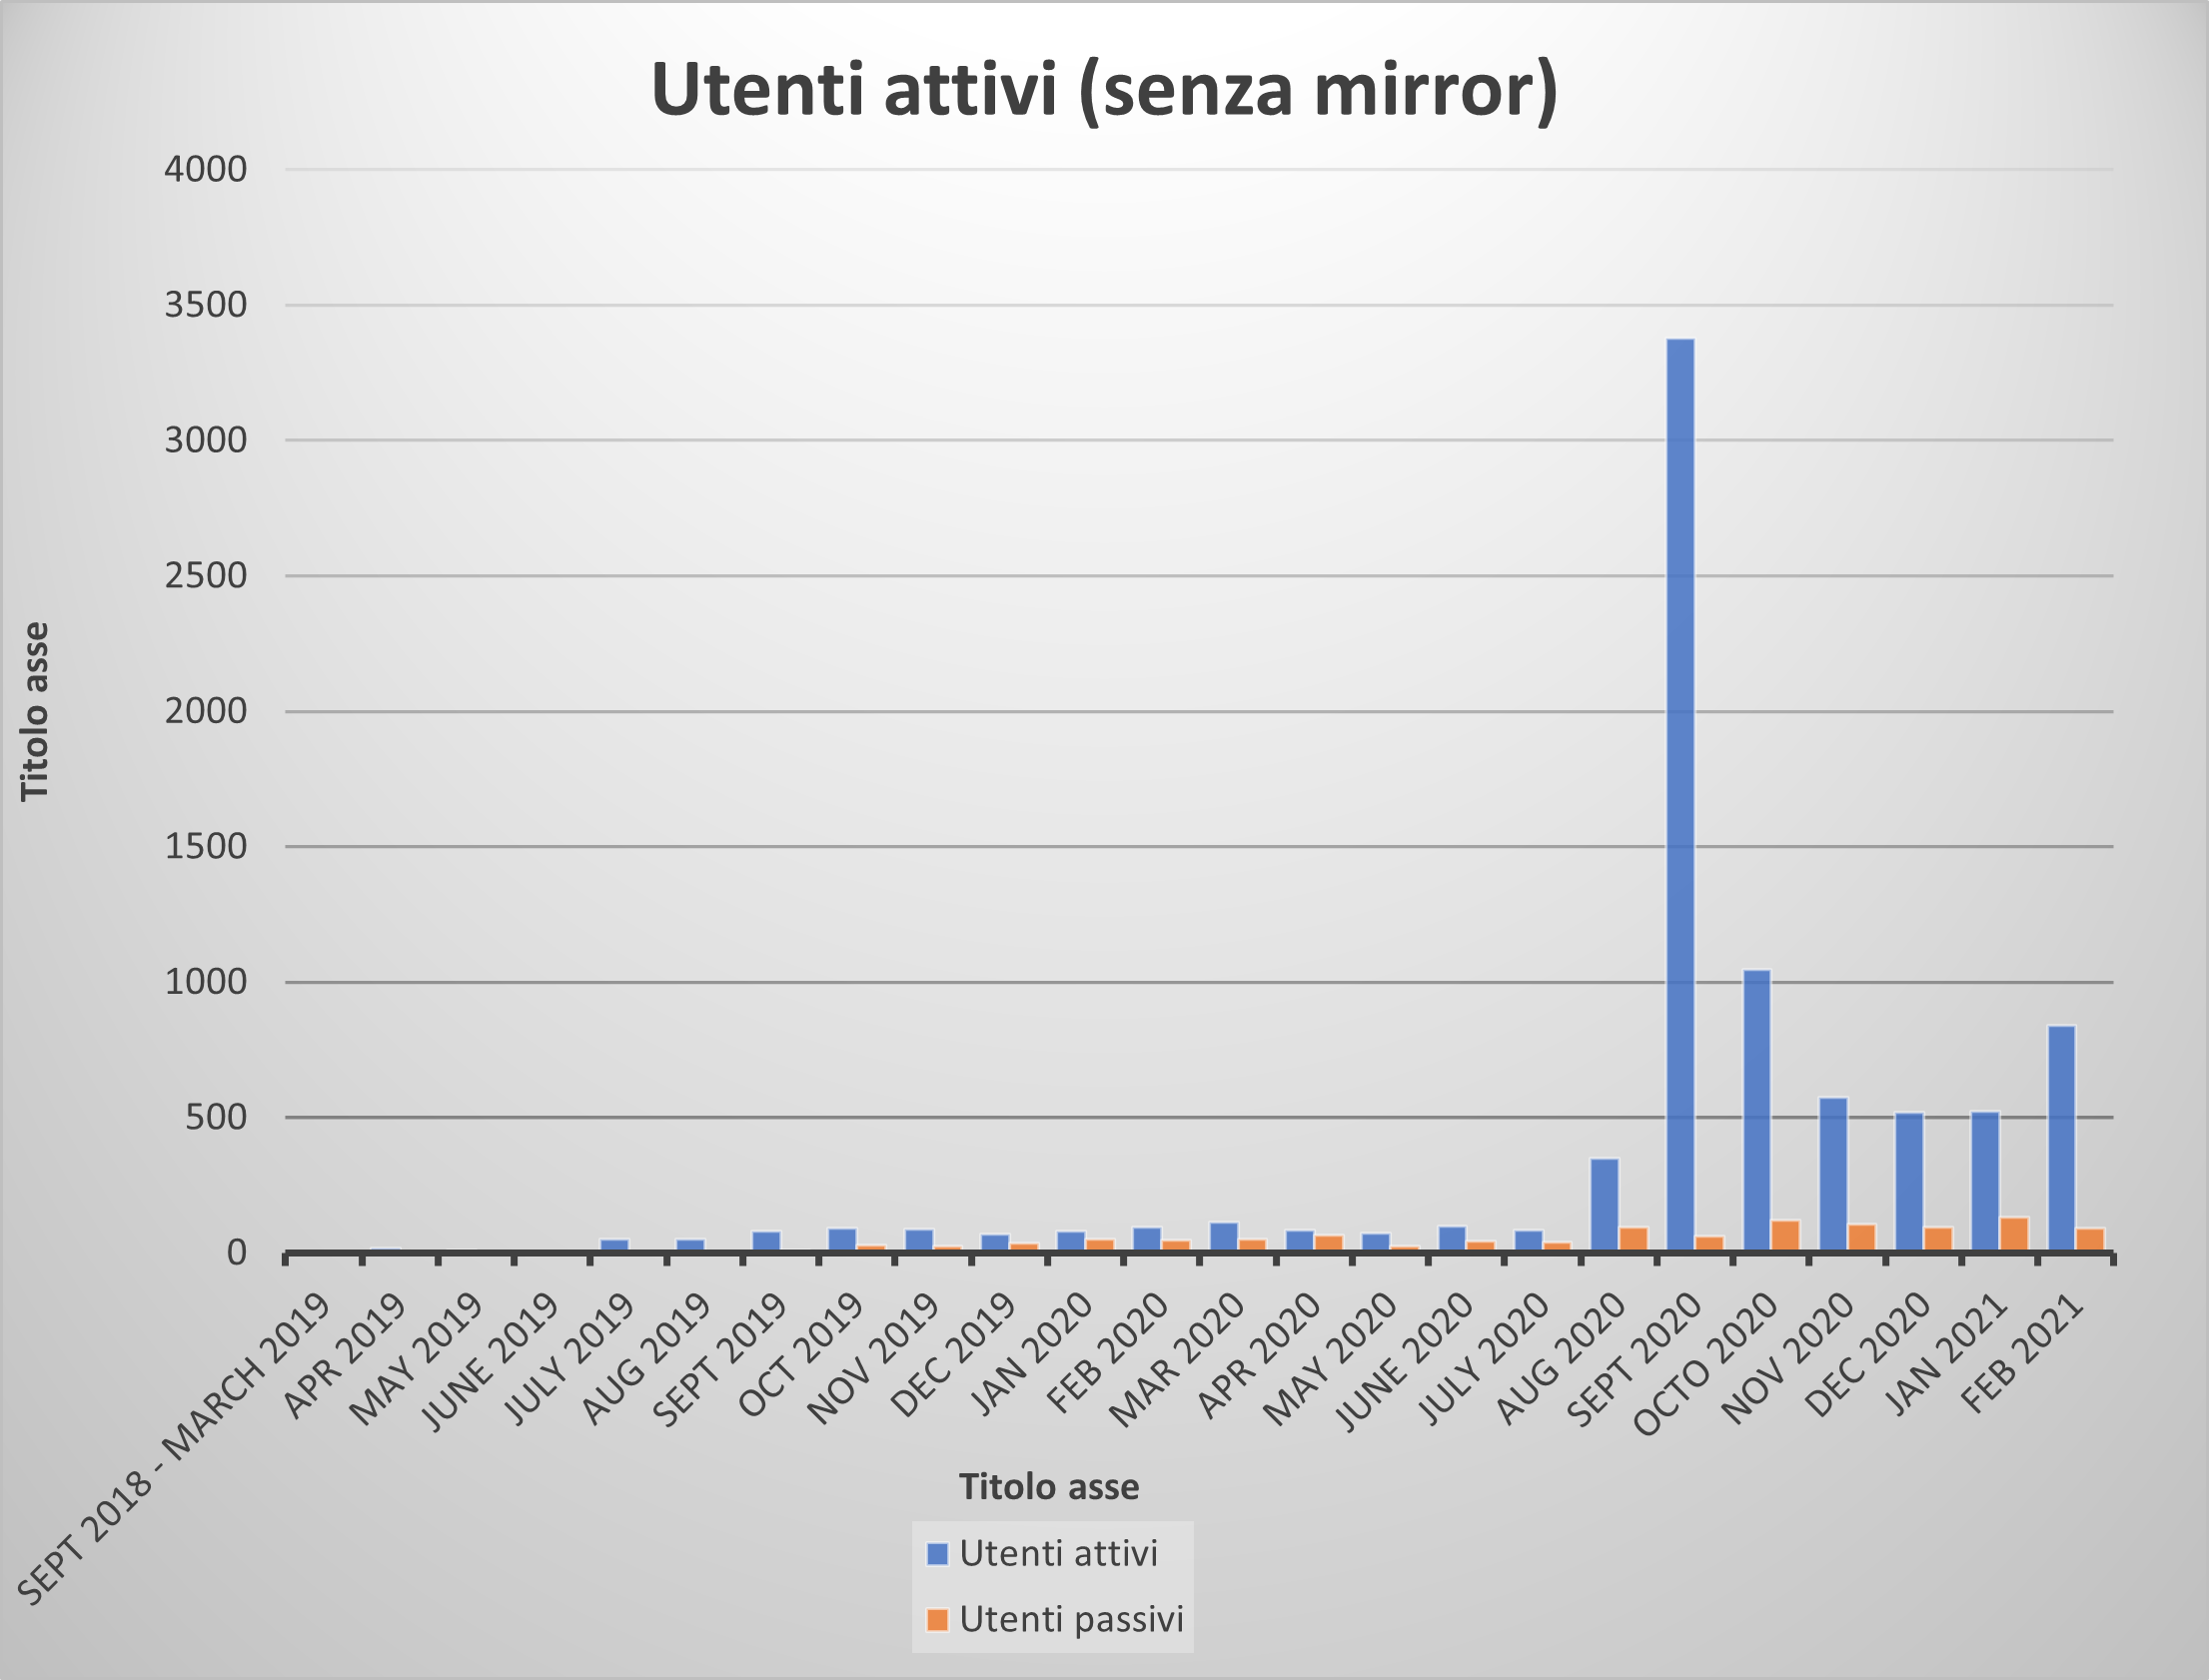
\includegraphics[width=0.7\textwidth]{graphs/utentiattivi_nomirr.png}
    \caption{Utenti attivi-passivi su base mensile escludendo account Mirror}
    \label{fig:attivi_nomirr}
\end{figure}

E' possibile notare come l'inclusione o l'esclusione degli account Mirror abbia un forte impatto sul conteggio degli account passivi. Confrontando le Figure constatiamo che, per la maggior parte degli account Mirror, non ci sia più un mirroring delle azioni che effettuano su Twitter, ma soltanto una continua ripetizione di azioni di login. A testimoniare questa supposizione vi è il fatto che, nel momento in cui consideriamo tali account, abbiamo un forte incremento degli account passivi in ogni mese. Inoltre, confrontando le Figure \ref{fig:attivi_conmirr} e \ref{fig:createacctMensile_conmirr}, possiamo notare come l'incremento di utenti attivi e passivi coincida proprio con i mesi nei quali abbiamo notato numerose inscrizioni di account Mirror, ovvero da Giugno 2020 a Settembre 2020.
D'altro canto, se consideriamo solo gli utenti non-Mirror, dopo il boom di iscrizioni rilevato nel mese di Settembre (vedi Figura \ref{fig:createacctMensile_nomirr}), il numero di utenti attivi rimane tra 500 e 1.000, mentre il numero di utenti inattivi rimane molto basso (Figura \ref{fig:attivi_nomirr}).

\section{Azioni di voto}
Dopo aver analizzato la natura dei vari account, insieme ad alcune caratteristiche chiave, come la creazione, volgiamo ora la nostra attenzione all'aspetto chiave della piattaforma Yup, ovvero i voti.
Come abbiamo visto nel Capitolo \ref{platform_chapter}, valutare i contenuti disponibili nel web è il motivo per cui Yup è stato proposto, e coincide inoltre con la maniera più importante per poter accumulare criptomoneta sulla piattaforma.
Questo impone di studiare in maniera dettagliata questa componente, e in particolare noi ci siamo concentrati sulle informazioni che i voti ci possono dare riguardo l'attività degli utenti e riguardo le piattaforme più valutate.

L'analisi dell'attività di votazione tiene conto delle sole azioni (createvote|v2|v3|v4 e postvote|v2|v3|v4), in quanto relative all'espressione di un voto.
Ricordiamo che le azioni createvote corrispondono a dei voti per contenuti precedentemente già votati almeno una volta, mentre le azioni postvote corrispondono a voti per contenuti precedentemente mai votati, come spiegato nel Capitolo \ref{platform_chapter}.
Anche in questo caso effettuiamo una distinzione tra quelle relative ad account Mirror e quelle relative ad account non-Mirror, mostrate in Tabella \ref{tab:votingactionsDistribution}.

\begin{table}
\centering
\begin{tabular}{ |c|c|c|c| }
 \hline
  & Totale & Mirror & non-Mirror \\
 \hline
 AZIONI DI VOTO & 497.526 & 180.371 & 317.155 \\
 \hline
 CREATEVOTE & 316.246 & 114.947 & 201.299 \\
 \hline
 POSTVOTE & 181.280 & 65.424 & 115.856 \\
 \hline
\end{tabular}
\caption{Distribuzione azioni di voto per account Mirror e non}
\label{tab:votingactionsDistribution}
\end{table}

La Tabella mostra che sotto il punto di vista della valutazione dei contenuti, gli account Mirror sono meno attivi rispetto agli account non-Mirror, nonostante il loro numero sia paragonabile, come mostrato in Tabella \ref{table:usersClassification}. Questo è principalmente dovuto al fatto che gli account Mirror sono account automatizzati e gestiti dagli sviluppatori di Yup al posto delle celebrità che questi account rappresentano e la loro attività deve rispecchiare l'account originale.
Notiamo inoltre che le azioni della famiglia createvote sono poco meno del doppio delle postvote.
Considerata la loro differente funzione, ci possiamo aspettare che le catene di voti formate da postvote e createvote siano corte e che in media per ogni postvote ci siano due createvote.


E' stato inoltre individuato un numero di votatori unici pari a \textbf{5.196}. Considerato come questo numero sia superiore a quello degli account non-Mirror creati tramite interazione con il protocollo (\textit{$3.475$}), ci porta alla conclusione che anche gli account che non sono stati originati da una createacct possono votare/utilizzare la piattaforma.


Di seguito mostriamo la distribuzione mensile delle azioni di voto includendo i Mirror, in Fgura \ref{fig:votingMensile_conmirr}, ed escludendo i Mirror in Figura \ref{fig:votingMensile_nomirr}.

\begin{figure}[t]
    \centering
    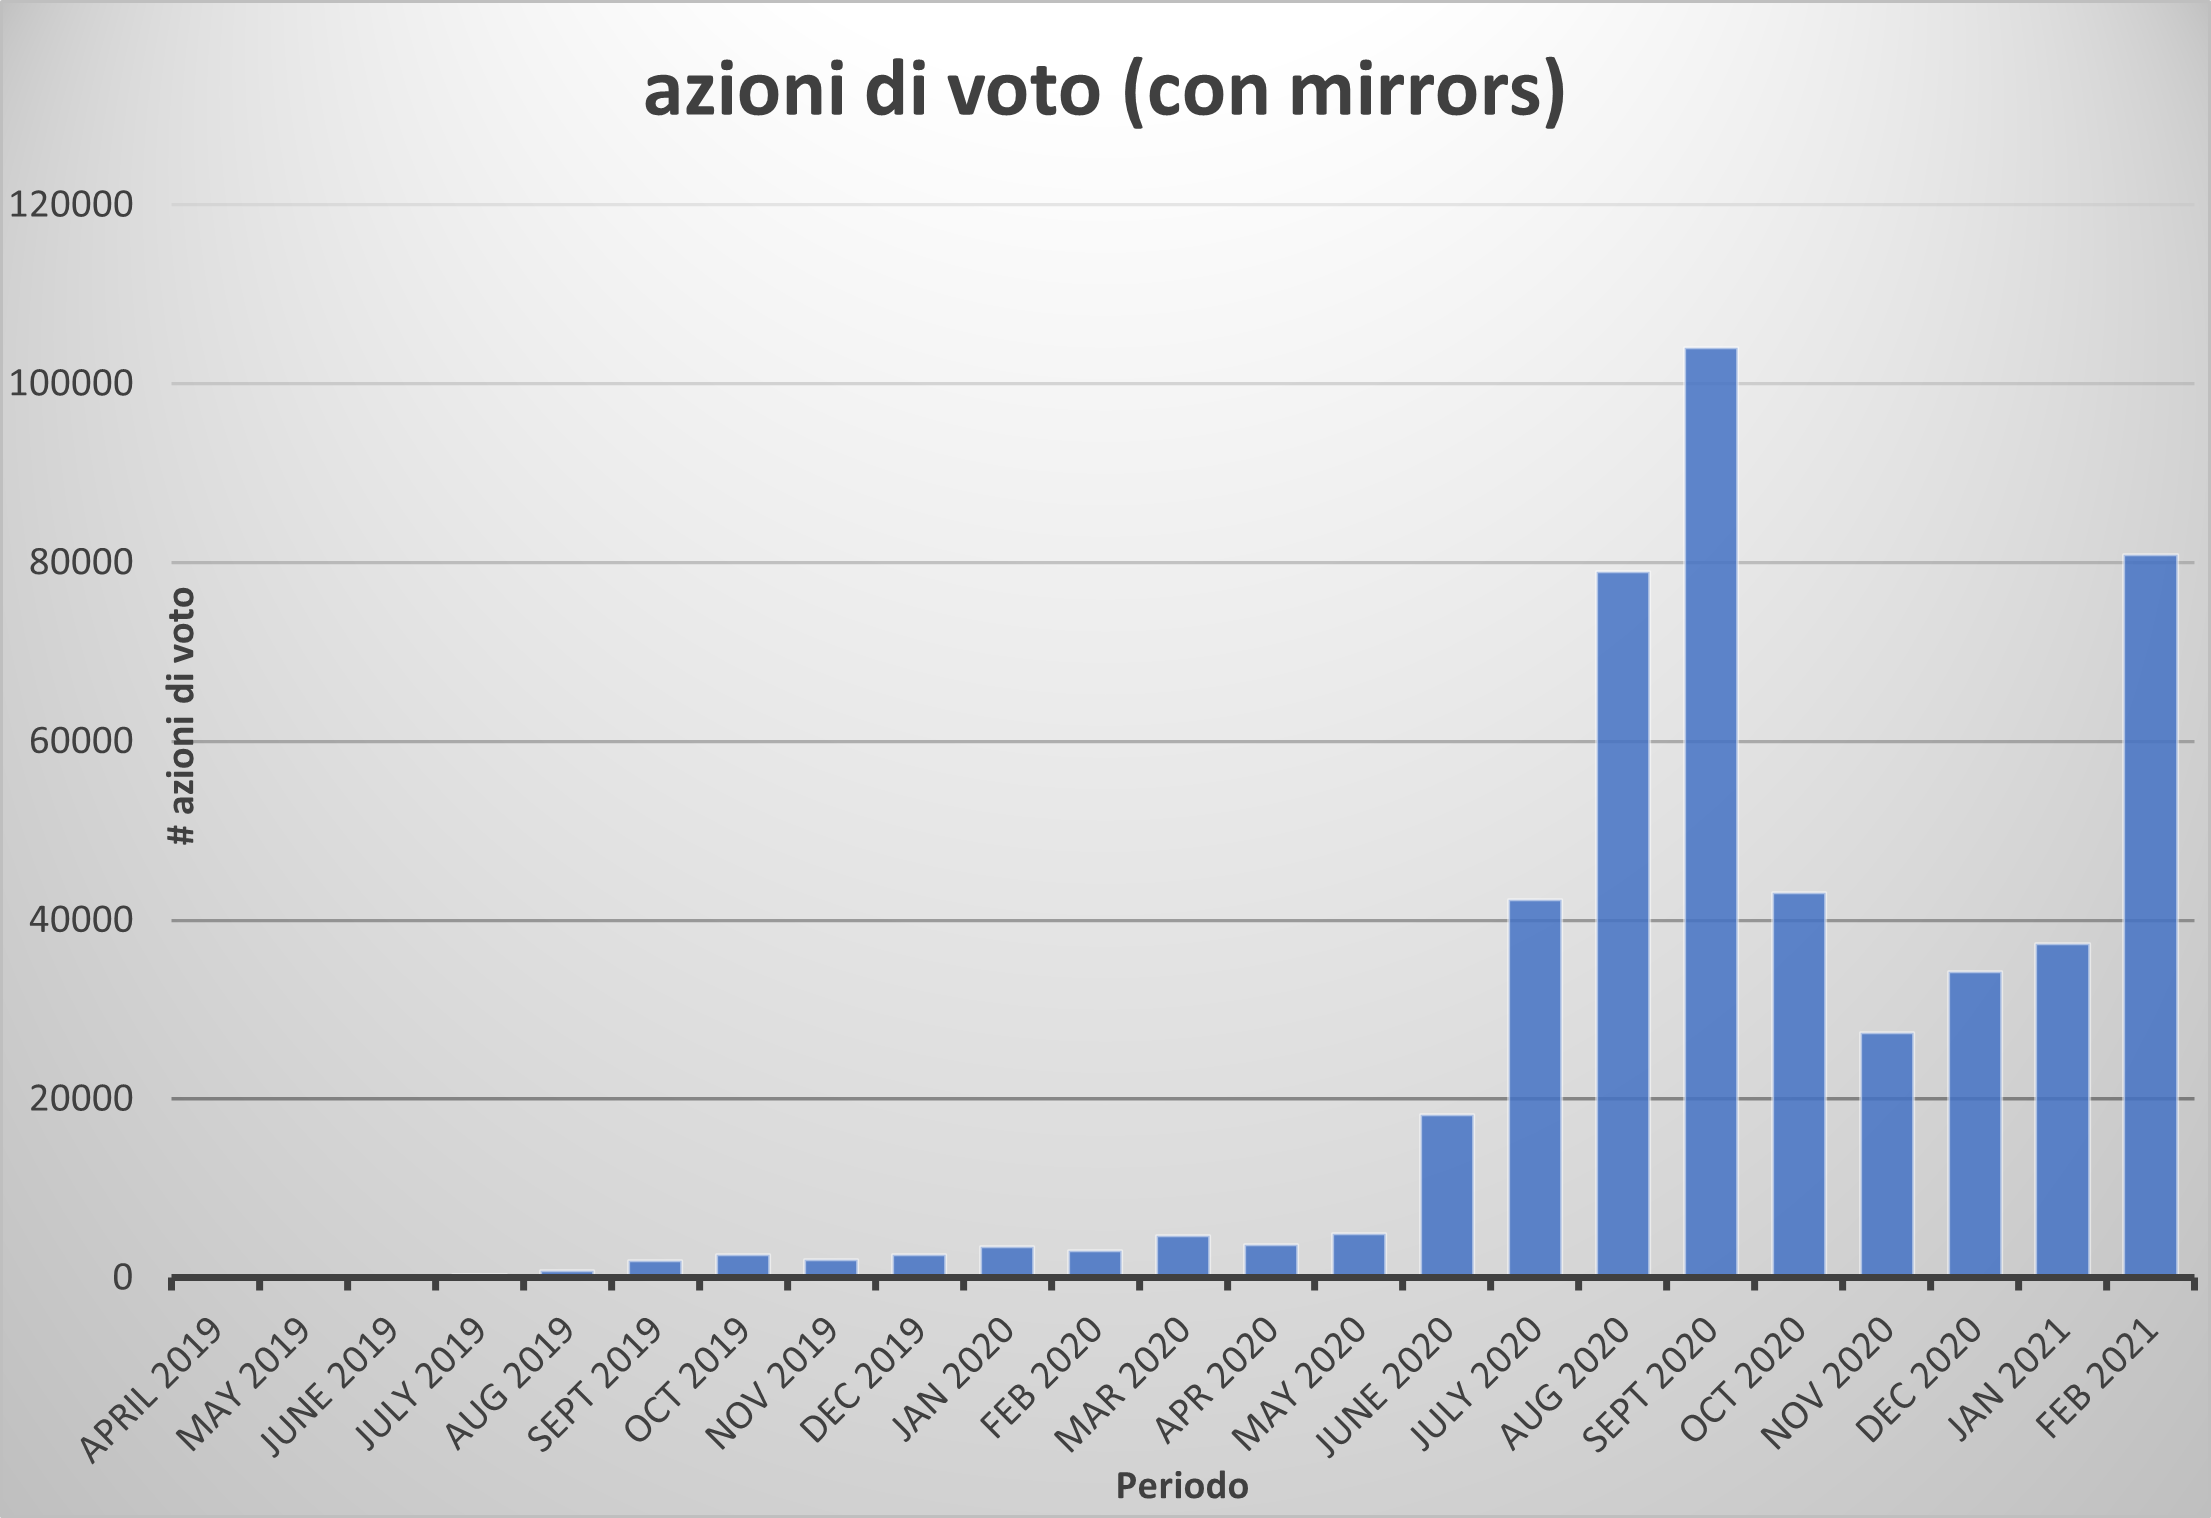
\includegraphics[width=.7\textwidth]{graphs/azioni_voto}
    \caption{Distribuzione mensile delle azioni di voto includendo account Mirror.}
    \label{fig:votingMensile_conmirr}
\end{figure}

\begin{figure}[t]
    \centering
    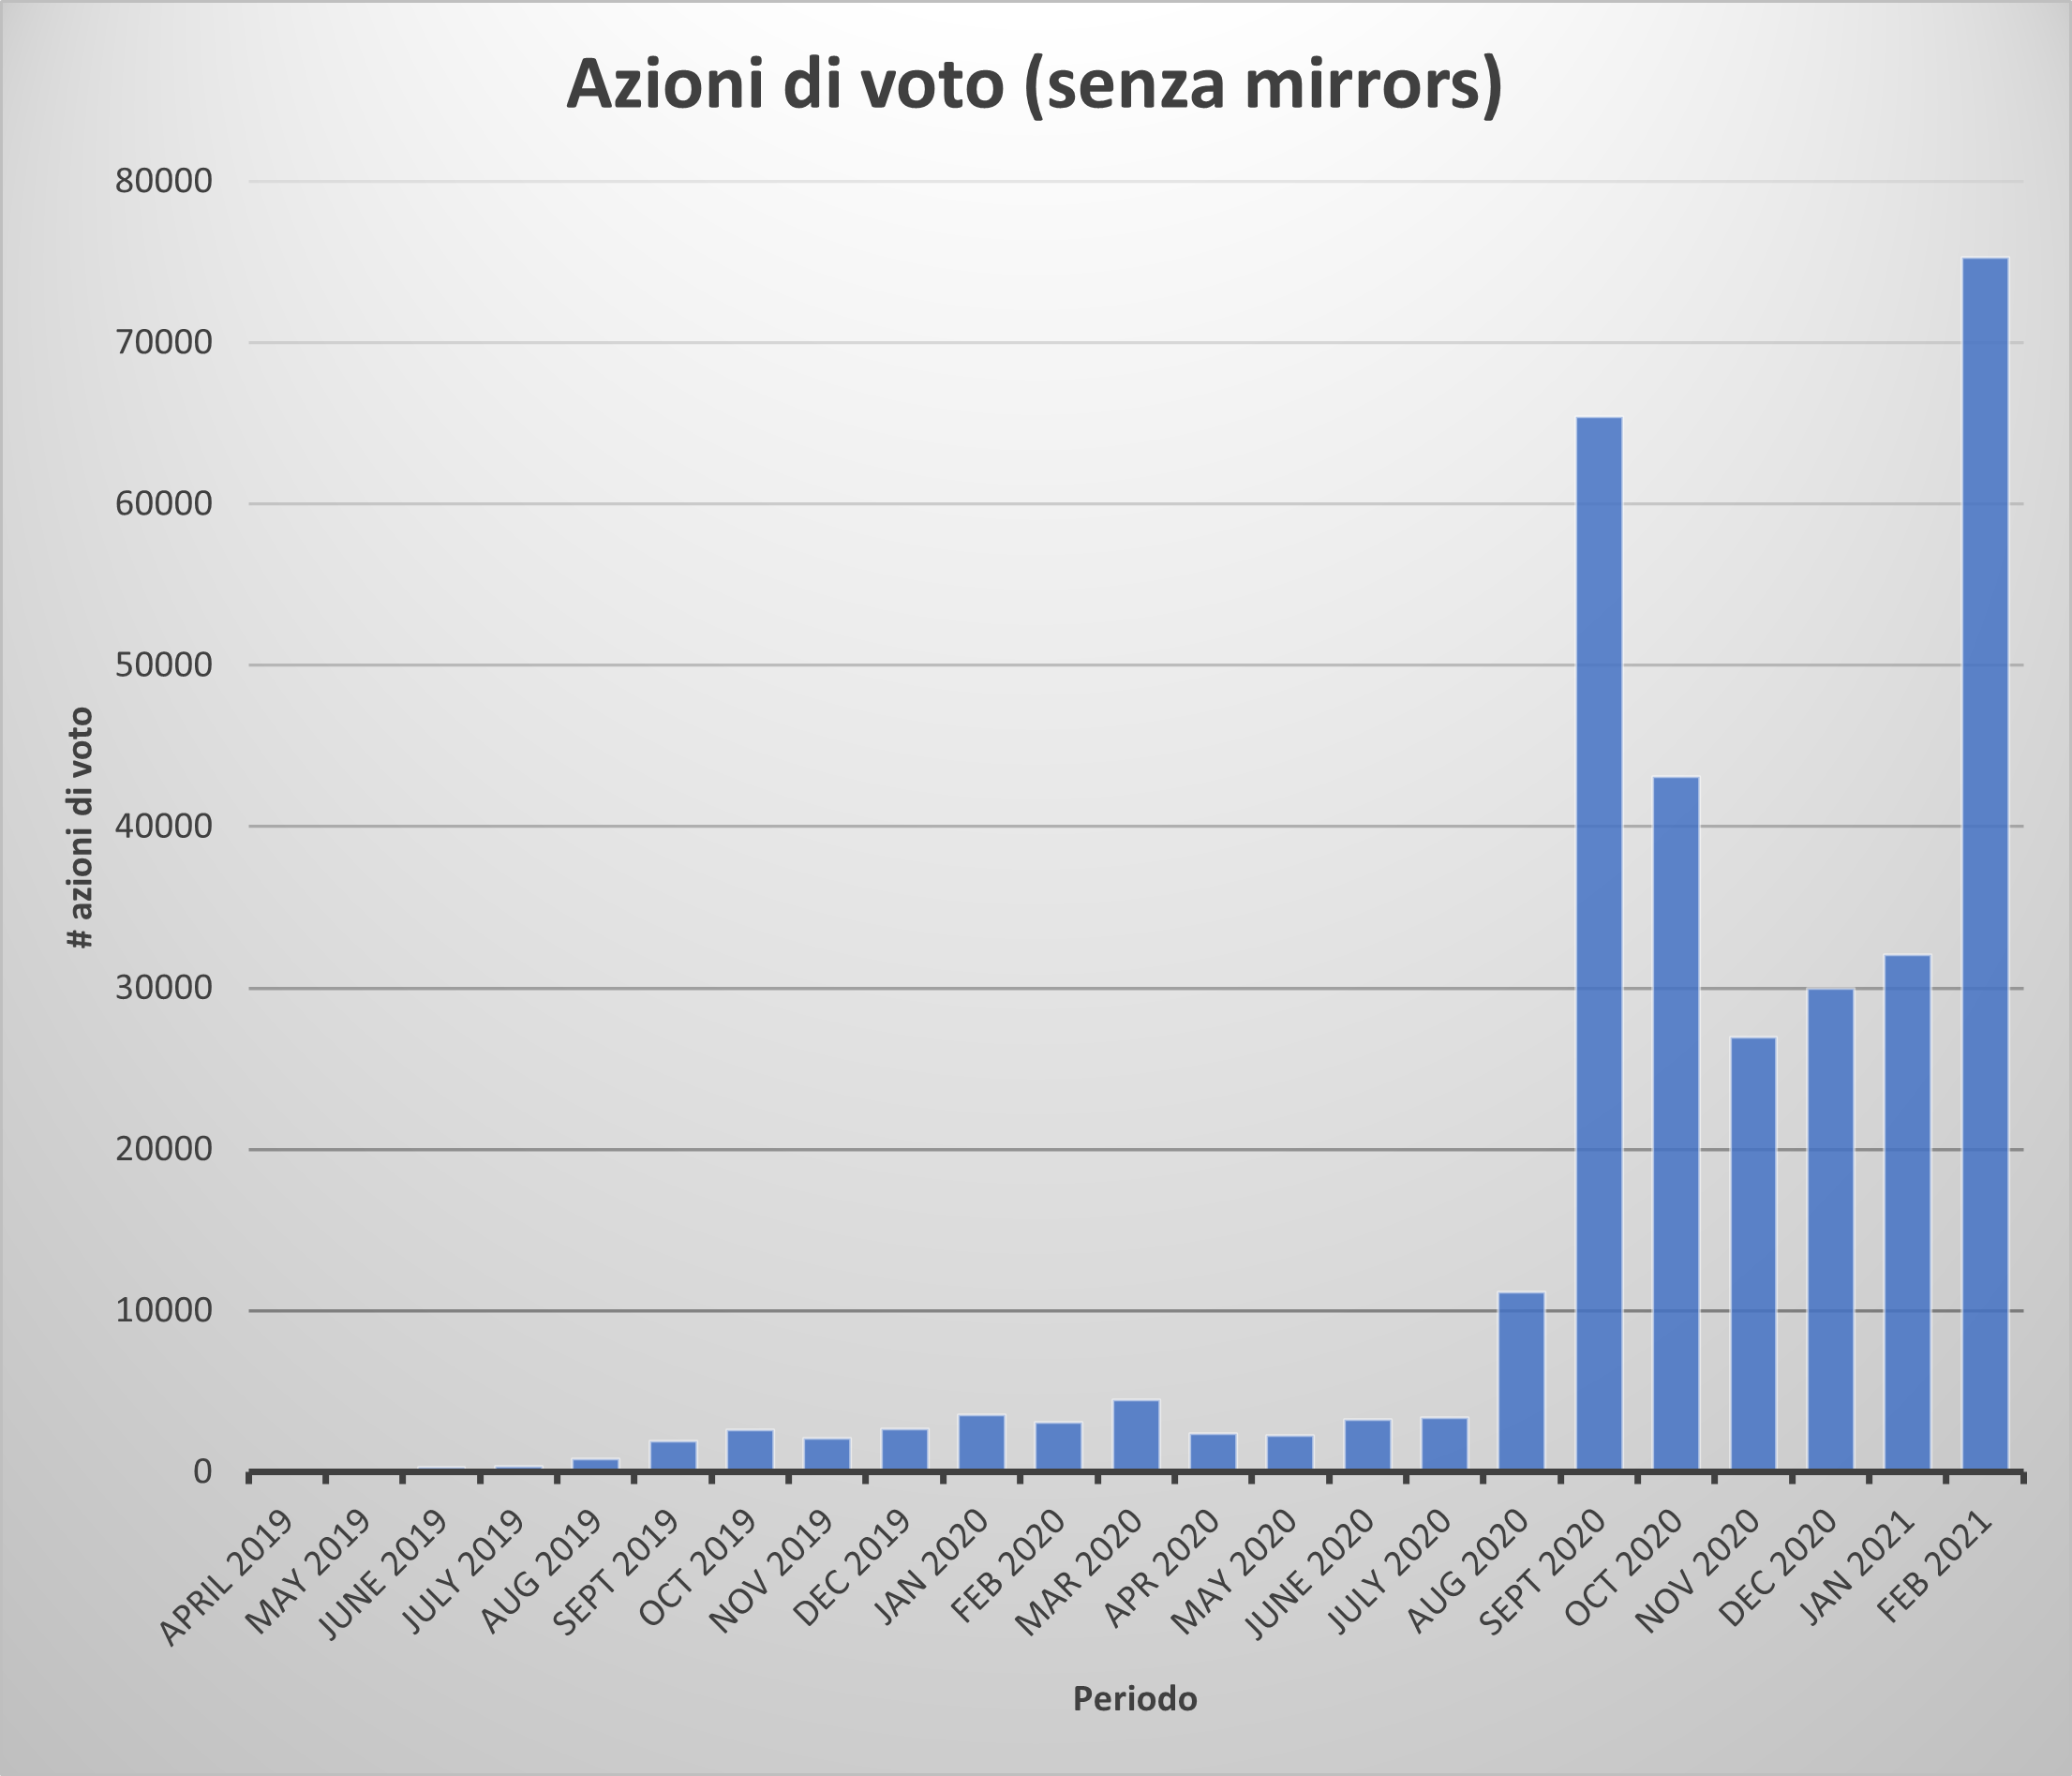
\includegraphics[width=.7\textwidth]{graphs/azioni_voto_nomirr}
    \caption{Distribuzione mensile delle azioni di voto escludendo account Mirror}
    \label{fig:votingMensile_nomirr}
\end{figure}

In questa analisi, come nelle precedenti, abbiamo un notevole incremento dell'attività nel periodo che precede il lancio della piattaforma. Notiamo infatti dei picchi notevoli nei mesi di Agosto e Settembre, che potremmo anche questa volta correlare al lancio di Yup, e successivamente nel mese di Febbraio, che testimonia una costante crescita dell'utilizzo del servizio da parte degli utenti.

Infine proponiamo una rappresentazione, sempre su base mensile, dei votatori unici individuati, ovvero utenti che hanno votato almeno un contenuto.
Mostriamo in Figura \ref{fig: uniquevoters_onlymirr} i votatori unici considerando solo account Mirror e in Figura \ref{fig: uniquevoters_nomirr} i votatori unici considerando solo account non-Mirror.

\begin{figure}[t]
    \centering
    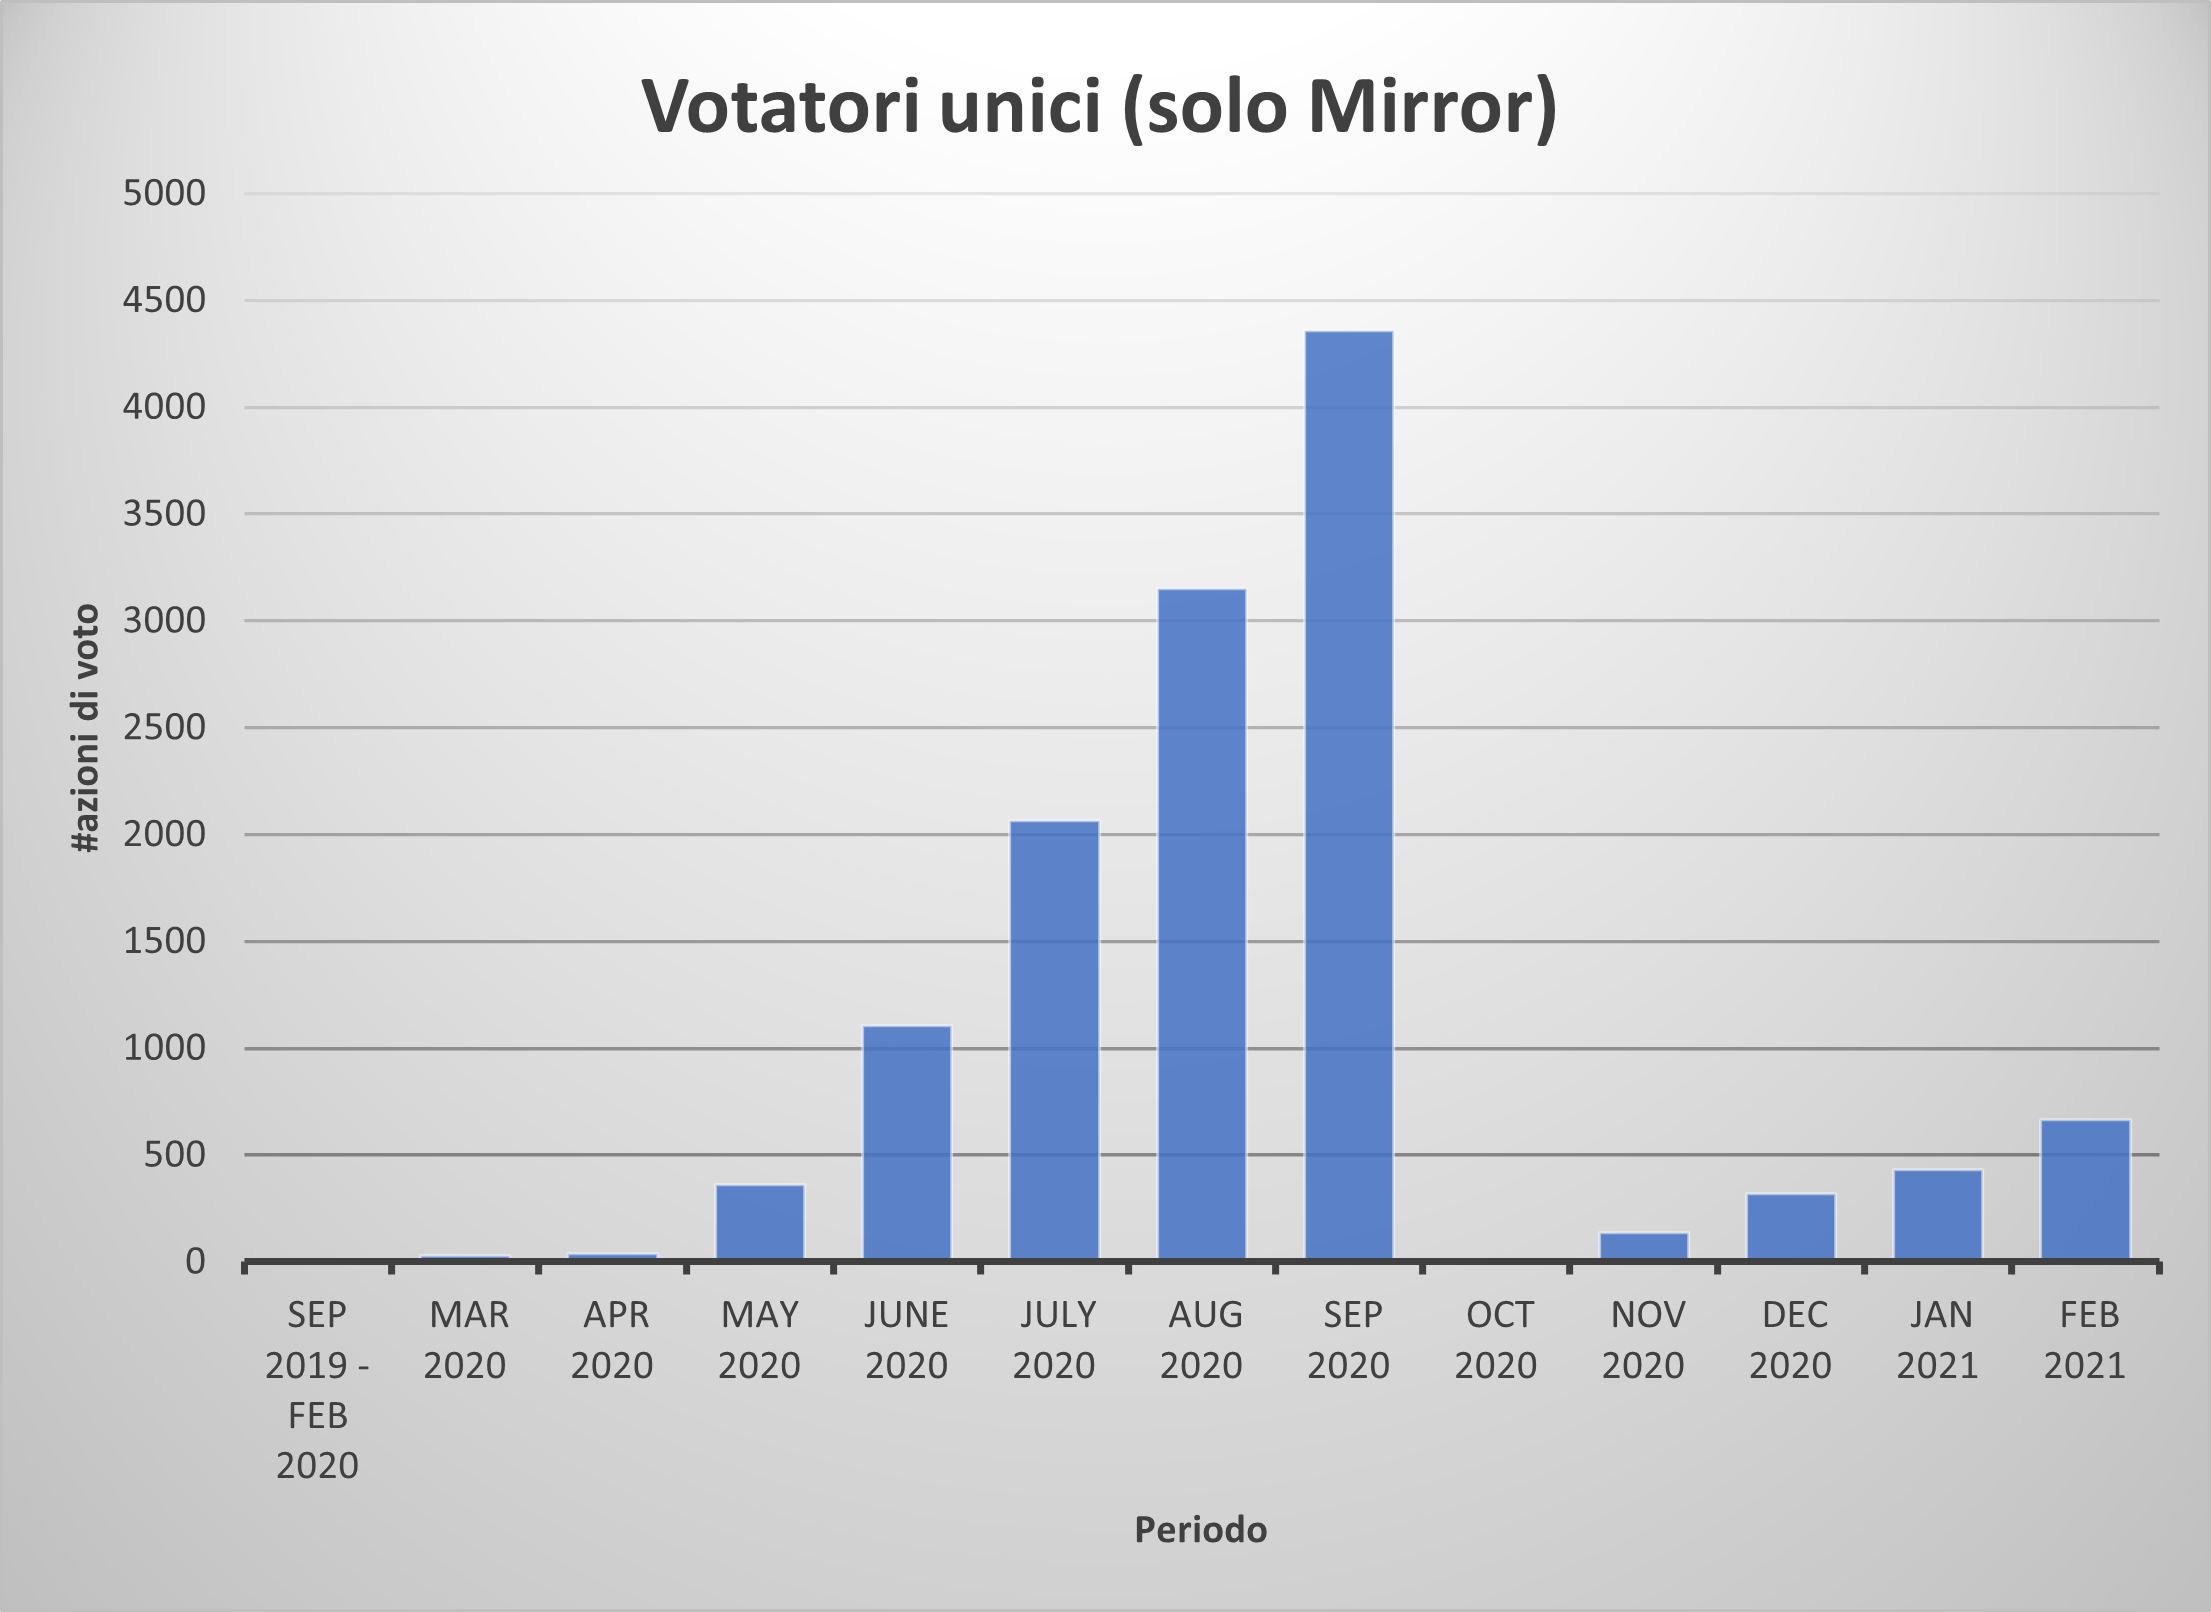
\includegraphics[width=.7\textwidth]{graphs/votatori_onlymirr.png}
    \caption{Rappresentazione mensile dei votatori unici, solo account Mirror}
    \label{fig: uniquevoters_onlymirr}
\end{figure}

\begin{figure}[t]
    \centering
    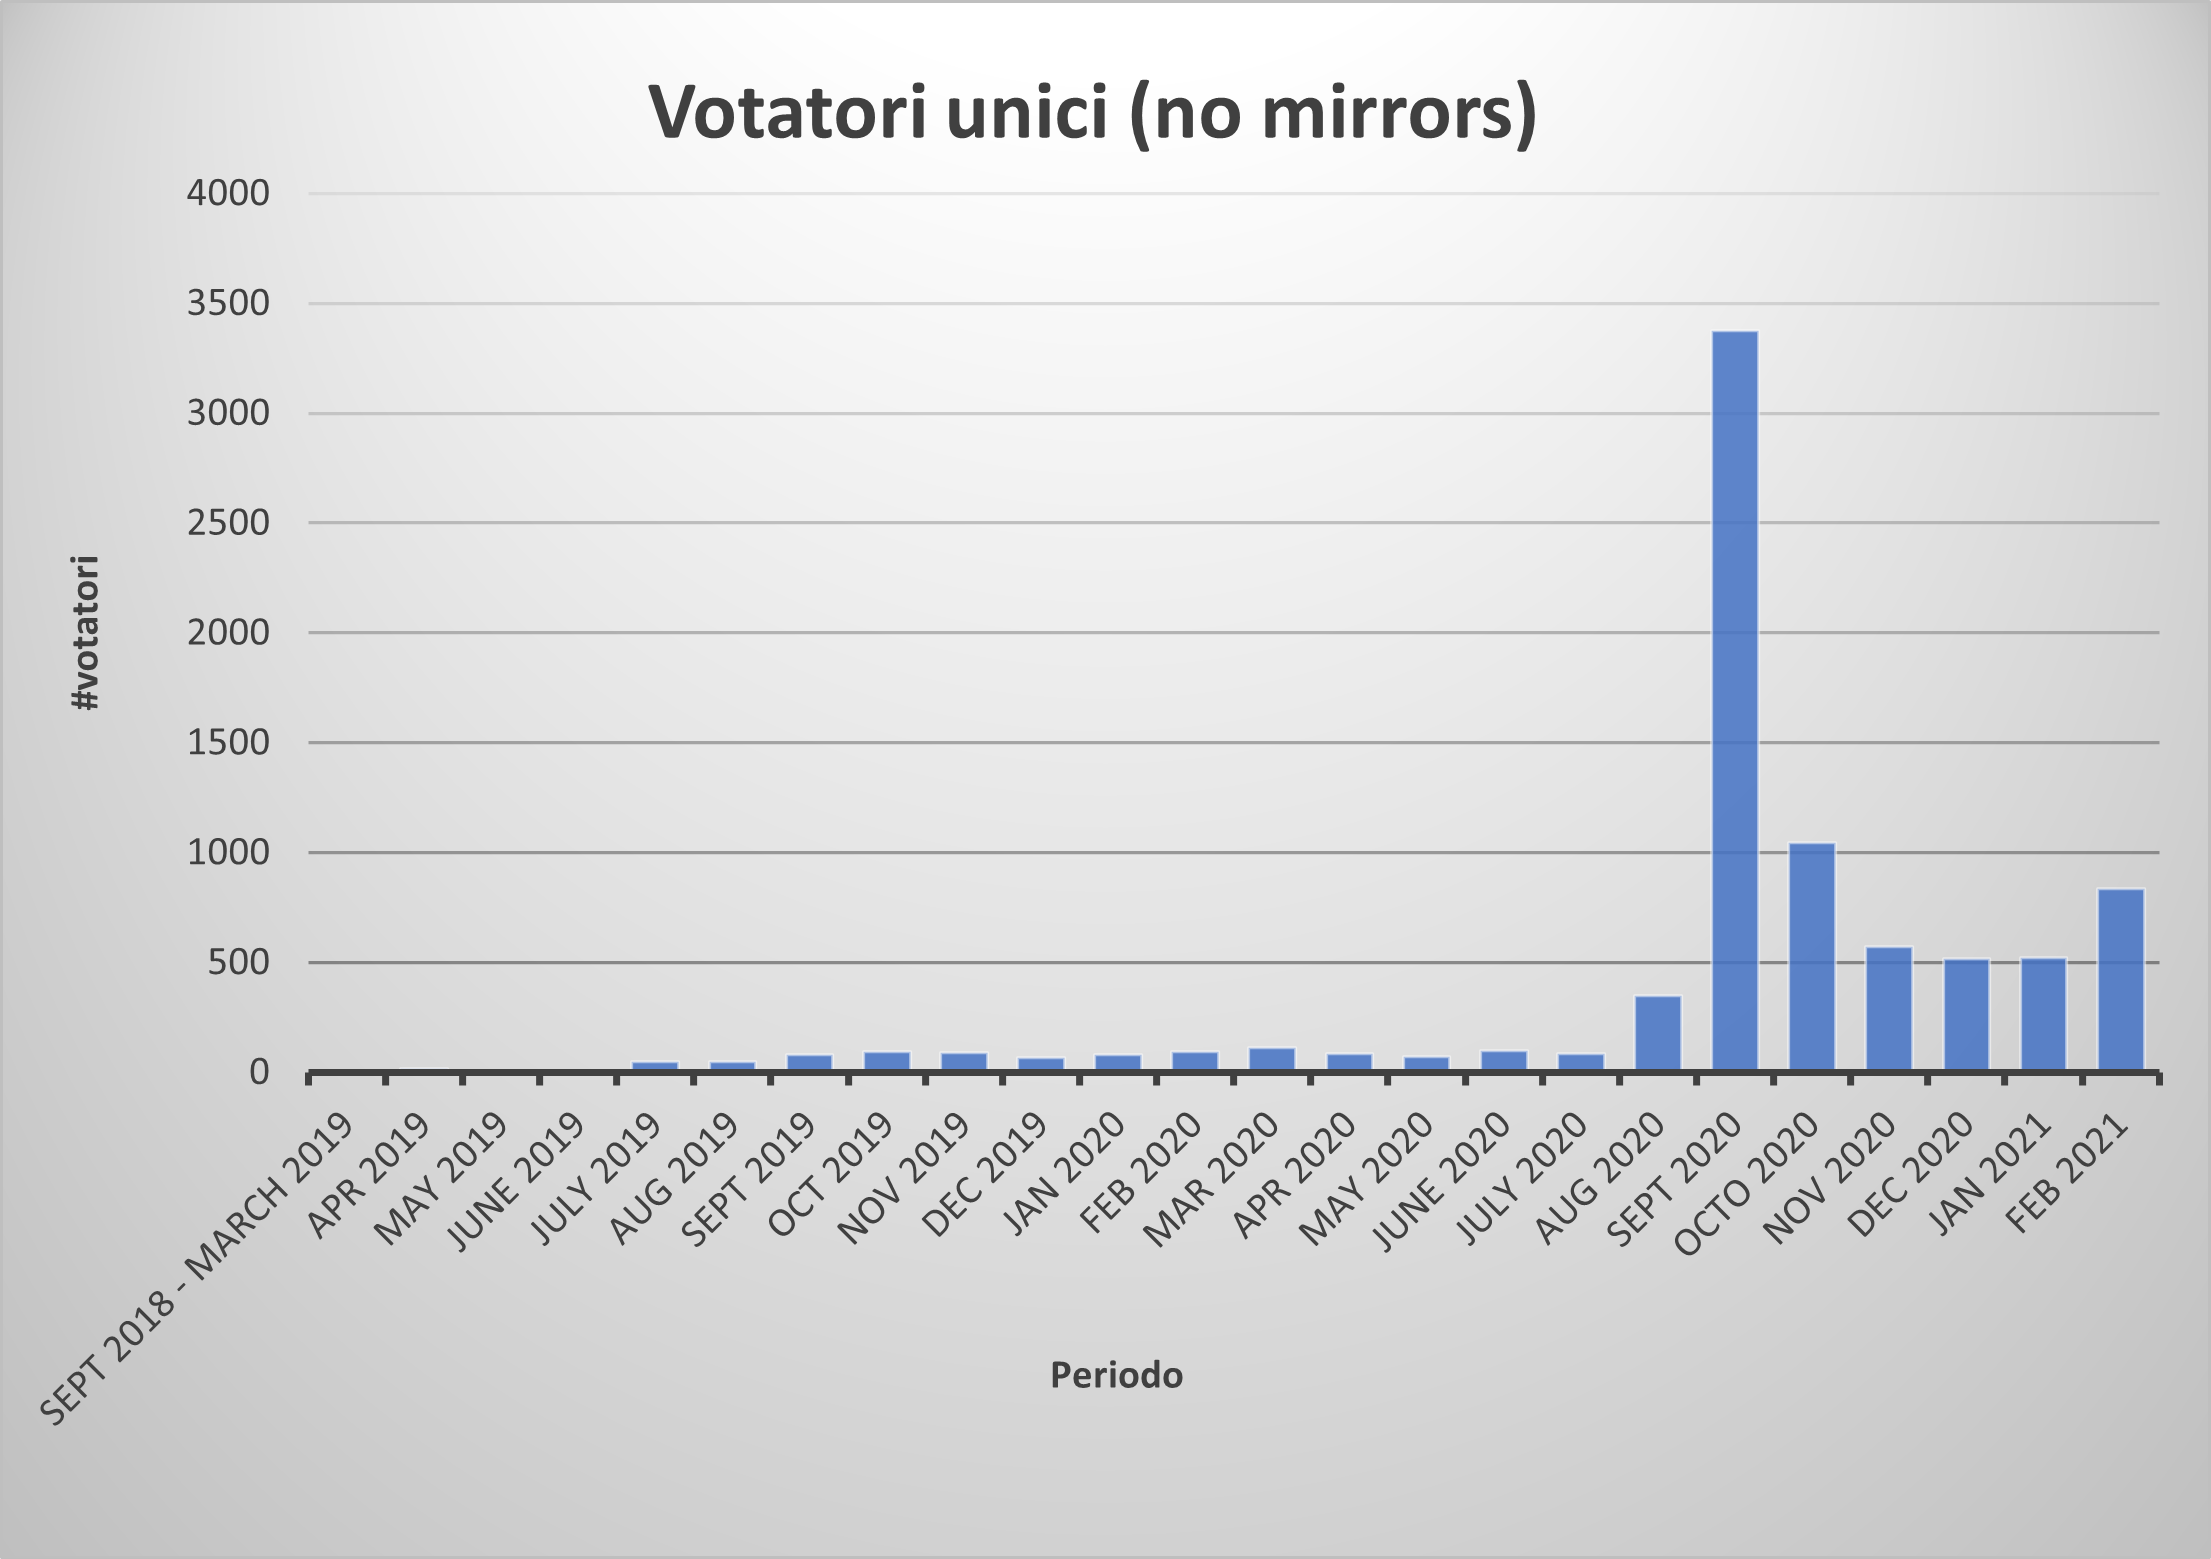
\includegraphics[width=.7\textwidth]{graphs/votatori_nomirr.png}
    \caption{Rappresentazione mensile dei votatori unici, solo account non-Mirror}
    \label{fig: uniquevoters_nomirr}
\end{figure}

Il grafico che considera solo account Mirror mostra che l'attività degli account Mirror ha subito un notevole decremento nel mese di Ottobre 2020, ovvero quando la fase Beta è ufficialmente terminata (Figura \ref{fig: uniquevoters_onlymirr}).
Ciononostante, l'attività dei Mirror è ricominciata a partire da Novembre 2020, e mostra una crescita costante.

Questo particolare si può osservare anche nella Figura \ref{fig: voting_onlymirr} che rappresenta, su base mensile, solo le azioni di voto effettuate da account Mirror. In questo caso abbiamo solo 5 azioni di voto nel mese di Ottobre 2020.

\begin{figure}[t]
    \centering
    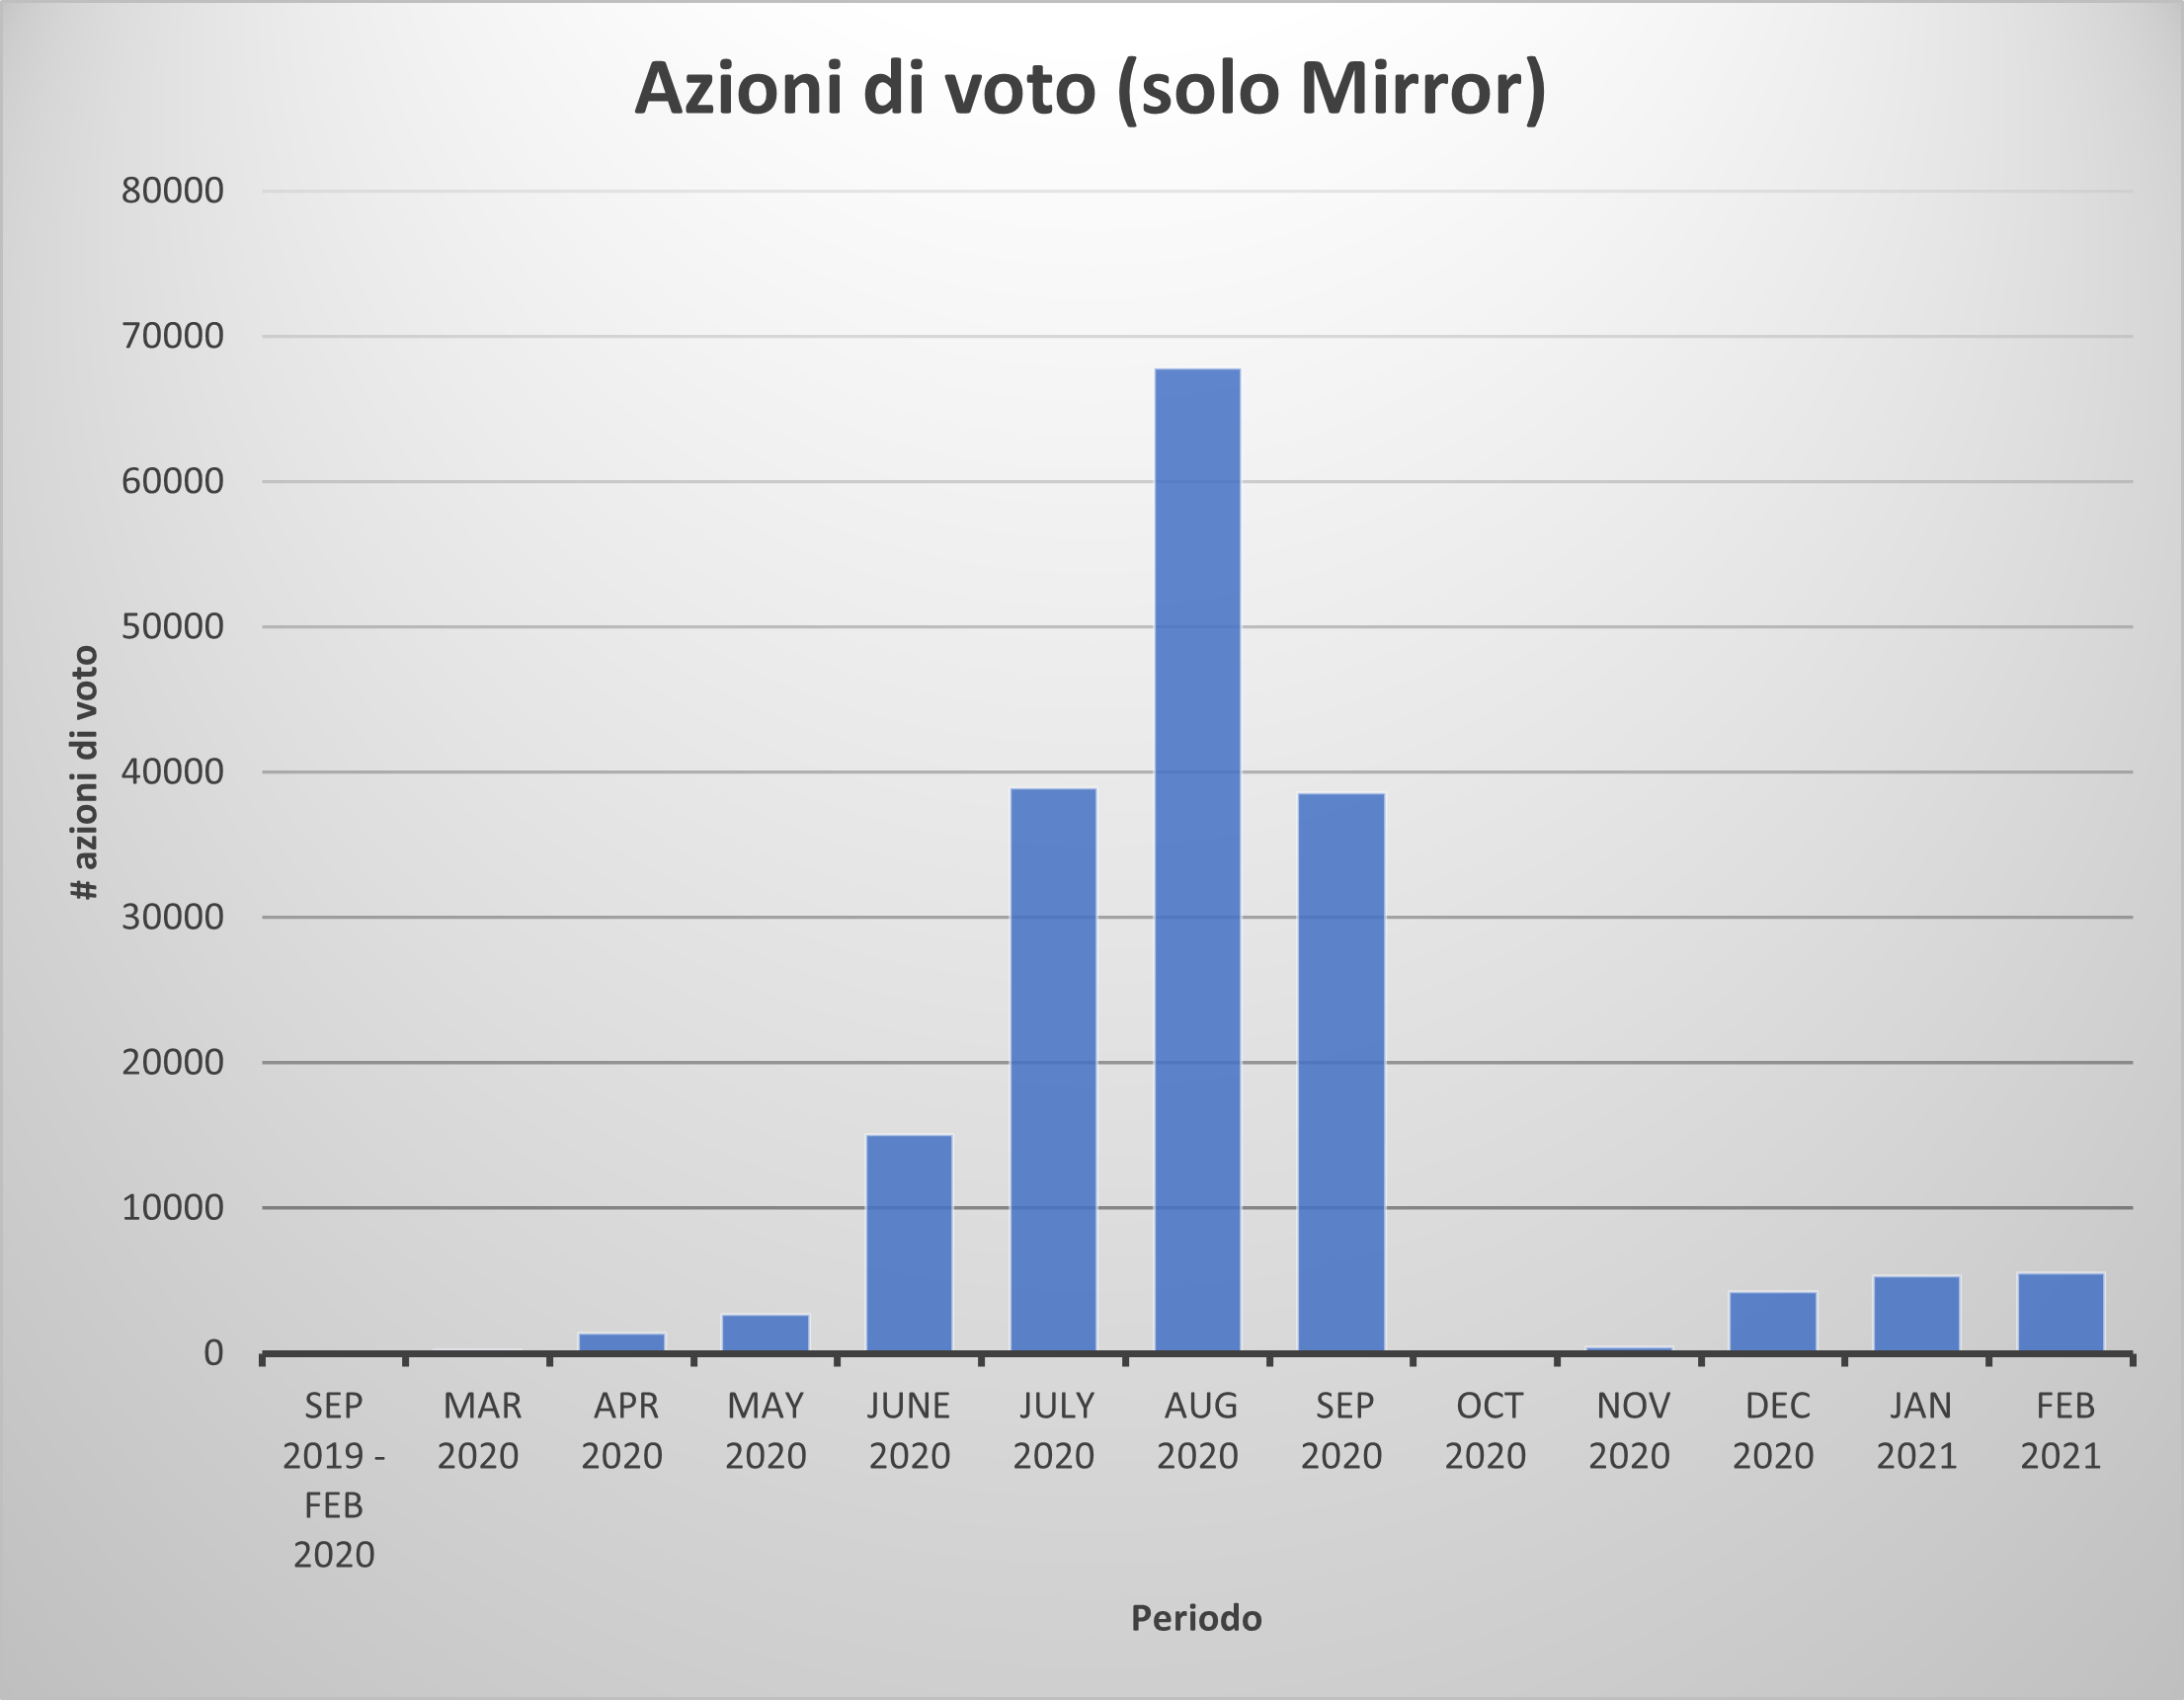
\includegraphics[width=.7\textwidth]{graphs/azioni_voto_onlymirr.png}
    \caption{Rappresentazione mensile delle azioni di voto, solo account Mirror}
    \label{fig: voting_onlymirr}
\end{figure}

Sembrerebbe che gli account Mirror inizialmente venissero ricompensati in qualità di creatori e successivamente questa funzionalità sia stata interrotta. Infatti le ultime ricompense assegnate ad account di questo tipo risalgono più o meno al mese di Luglio del 2020. Questo avvalora l'ipotesi che le ricompense creatore vengano momentaneamente accumulate sull'account \textbf{yupcreators1} con l'obiettivo di essere successivamente distribuite quando più creatori si "iscriveranno" effettivamente alla piattaforma.

\subsection{Distribuzione piattaforme}
\label{platoforms_section}
Ci concentriamo ora nello studio delle piattaforme i cui contenuti sono più comunemente votati su Yup.
Con lo scopo di effettuare un'analisi della distribuzione dei voti sulle varie piattaforme, da qui in poi considereremo solo le azioni di voto di account non-Mirror e per cui è stato possibile risalire al contenuto.
Esistono infatti alcuni casi in cui il postid relativo ad una createvote (link al voto antecedente in senso temporale) non era più presente all'interno del database, probabilmente perché il voto precedente è stato eliminato.
La scelta di concentrarci sui solo account non-Mirror deriva dal fatto di considerare azioni umane fatte sulla piattaforma, invece che considerare anche azioni non umane degli account Mirror.
Dalle nostre analisi, abbiamo individuato un numero di piattaforme uniche votate pari a \textbf{1.884}, che è un segno del fatto che utenti appartenenti a molte piattaforme sono interessate al concetto proposto da Yup.
\\
\\
In Figura \ref{fig: platformsunique_nomirr} mostriamo una rappresentazione delle piattaforme in cui sono stati votati il maggior numero di contenuti unici, mentre in Figura \ref{fig: platformstot_nomirr} mostriamo il numero di voti totali per i contenuti raggruppati per piattaforma.
Per una più facile comprensione dei grafici raggruppiamo in un'unica voce, \textbf{others}, i dati relativi alle piattaforme che non rientrano nelle 10 più importanti.

\begin{figure}[t]
    \centering
    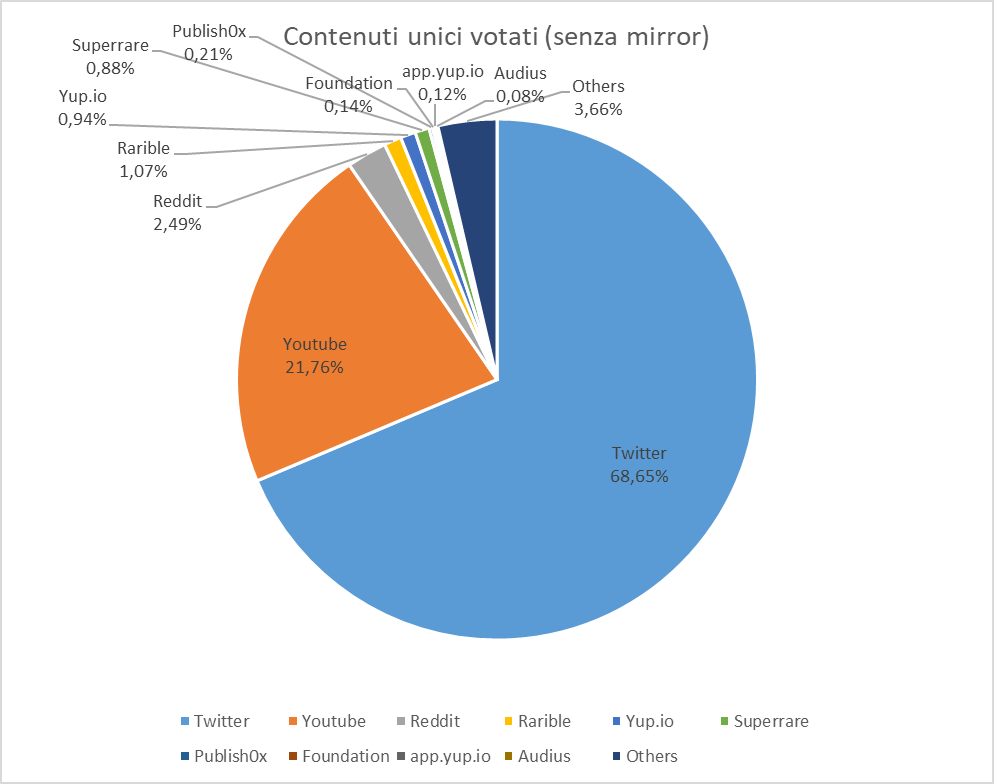
\includegraphics[width=0.7\textwidth]{graphs/platforms_unici_nomirr.png}
    \caption{Distribuzione dei contenuti votati sulle varie piattaforme escludendo account mirrors}
    \label{fig: platformsunique_nomirr}
\end{figure}    
    %\vspace*{\floatstep}
\begin{figure}[t]  
    \centering
    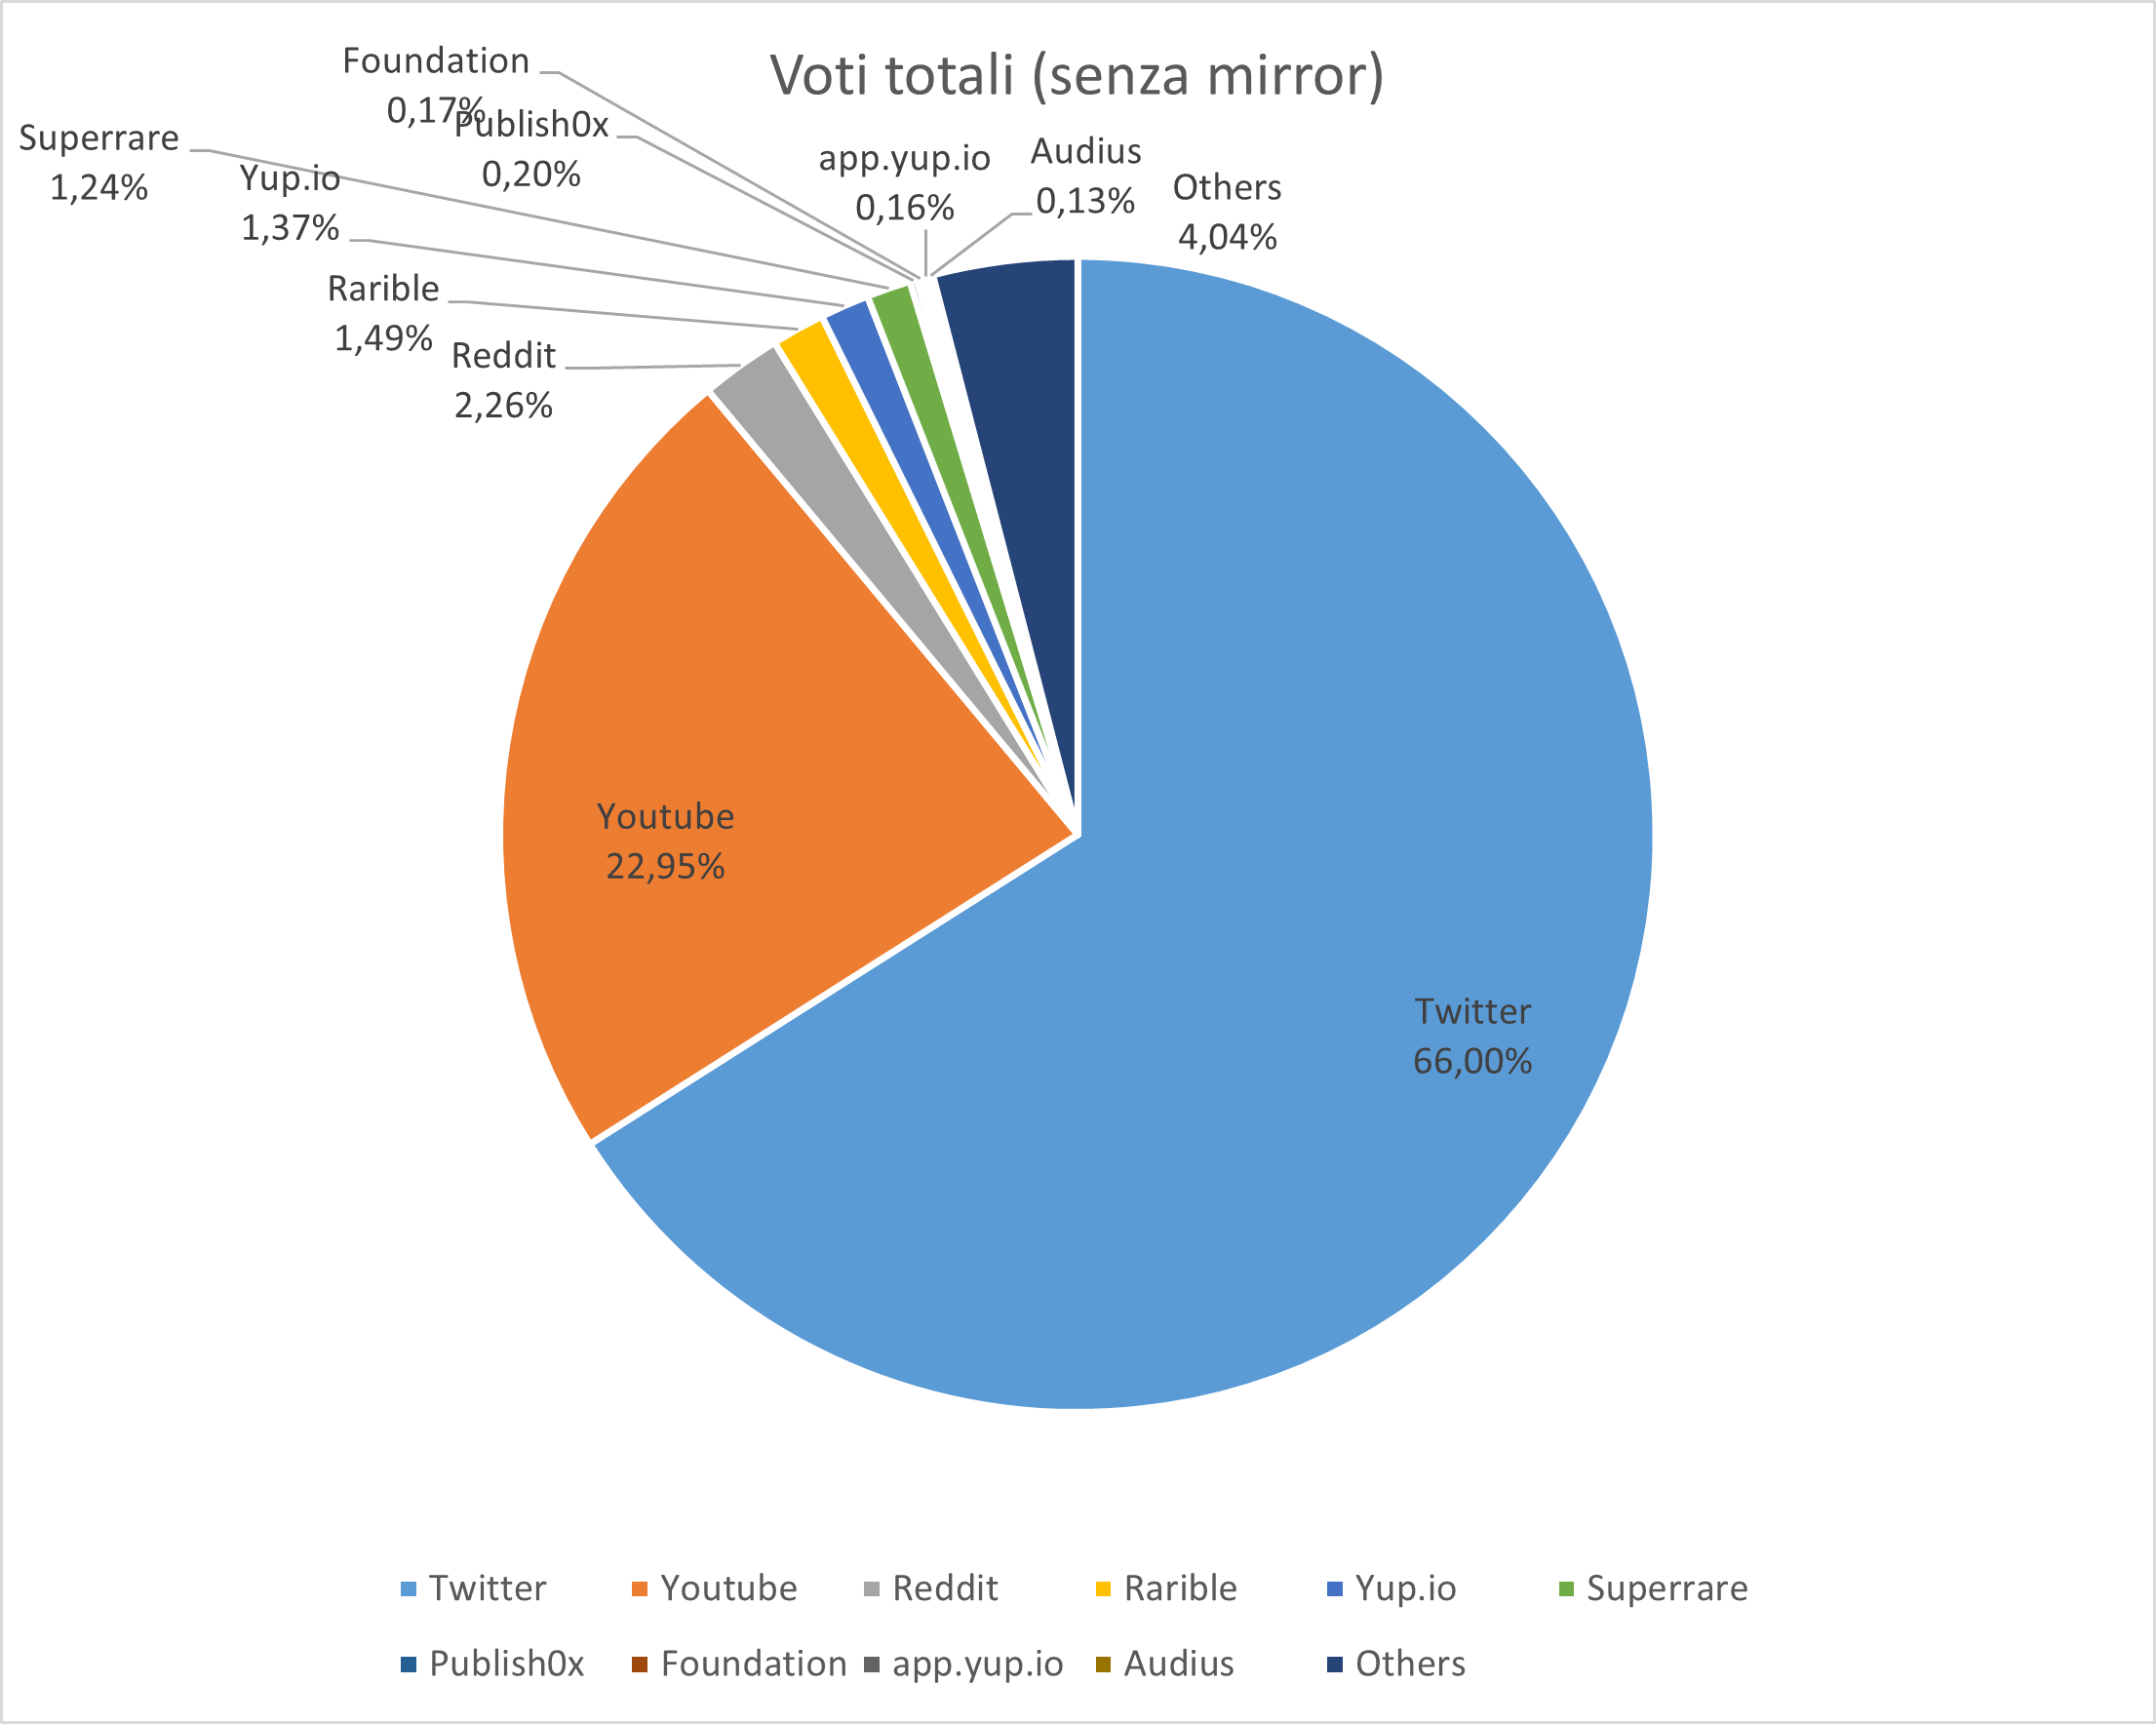
\includegraphics[width=0.7\textwidth]{graphs/platforms_tot_nomirr.png}
    \caption{Distribuzione dei voti totali sulle varie piattaforme escludendo account mirrors}
    \label{fig: platformstot_nomirr}
\end{figure}
%

Dalle Figure si può notare come le piattaforme integrate con l'estensione (Twitter, Youtube e Reddit) si trovino ai vertici della classifica. L'unica che costituisce una eccezione è Google Maps, la quale non compare nemmeno tra le 10 piattaforme più popolari. Continuando su questo aspetto, è interessante come siano presenti numerose piattaforme in ambito cripto, nonostante non supportino ancora l'overlay. In particolare, citiamo Rarible, Superrare e Foundation per quanto riguarda compravendita o in genere discussione su NFT; Publish0x è invece una piattaforma di blogging che ricompensa i propri utenti in criptovaluta e il cui sistema di ricompensa è basato su Ethereum; Audius, corrispettivo cripto di Spotify che distribuisce ricompense agli artisti, implementato su Ethereum.


Con l'obiettivo di avere risultati più specifici per i voti effettuati sulle principali piattaforme integrate, abbiamo indagato la distribuzione dei voti sui vari profili (Twitter), canali (Youtube) e subreddit (Reddit).
Questo ci permetterà di capire quali sono gli argomenti che catturano l'attenzione, ed in particolare i personaggi più seguiti, dagli utenti di Yup.
Mostriamo in Tabella \ref{tab: profiles_votes} il numero di profili Twitter, canali Youtube e subreddit votati almeno una volta da utenti Yup.

\begin{table}[h!]
\centering
\begin{tabular}{ |c|c|}
\hline
PROFILI TWITTER & 29.880 \\
\hline
CANALI YOUTUBE & 3.897 \\
\hline
SUBREDDITS & 628 \\
\hline
\end{tabular}
\caption{Profili unici votati}
\label{tab: profiles_votes}
\end{table}

In particolare notiamo come i profili Twitter siano di gran lunga più comune, probabilmente grazie alla notorietà della piattaforma e alla possibilità di includere in un singolo contenuto (tweet) testo, immagini, link e video.

Di seguito mostriamo i grafici del numero di voti dei 10 profili Twitter più votati (Figura \ref{fig: twitter_profiles}), dei 10 canali Youtube più votati (Figura \ref{fig: youtube_channels}) e dei 10 subreddit più votati \ref{fig: reddit_subreddits}. Anche in questo caso mostriamo solamente i 10 account con maggior numero di voti per motivi di comprensione e includiamo i dati di tutti gli elementi restanti in \textbf{others}.

\begin{figure}[t]
    \centering
    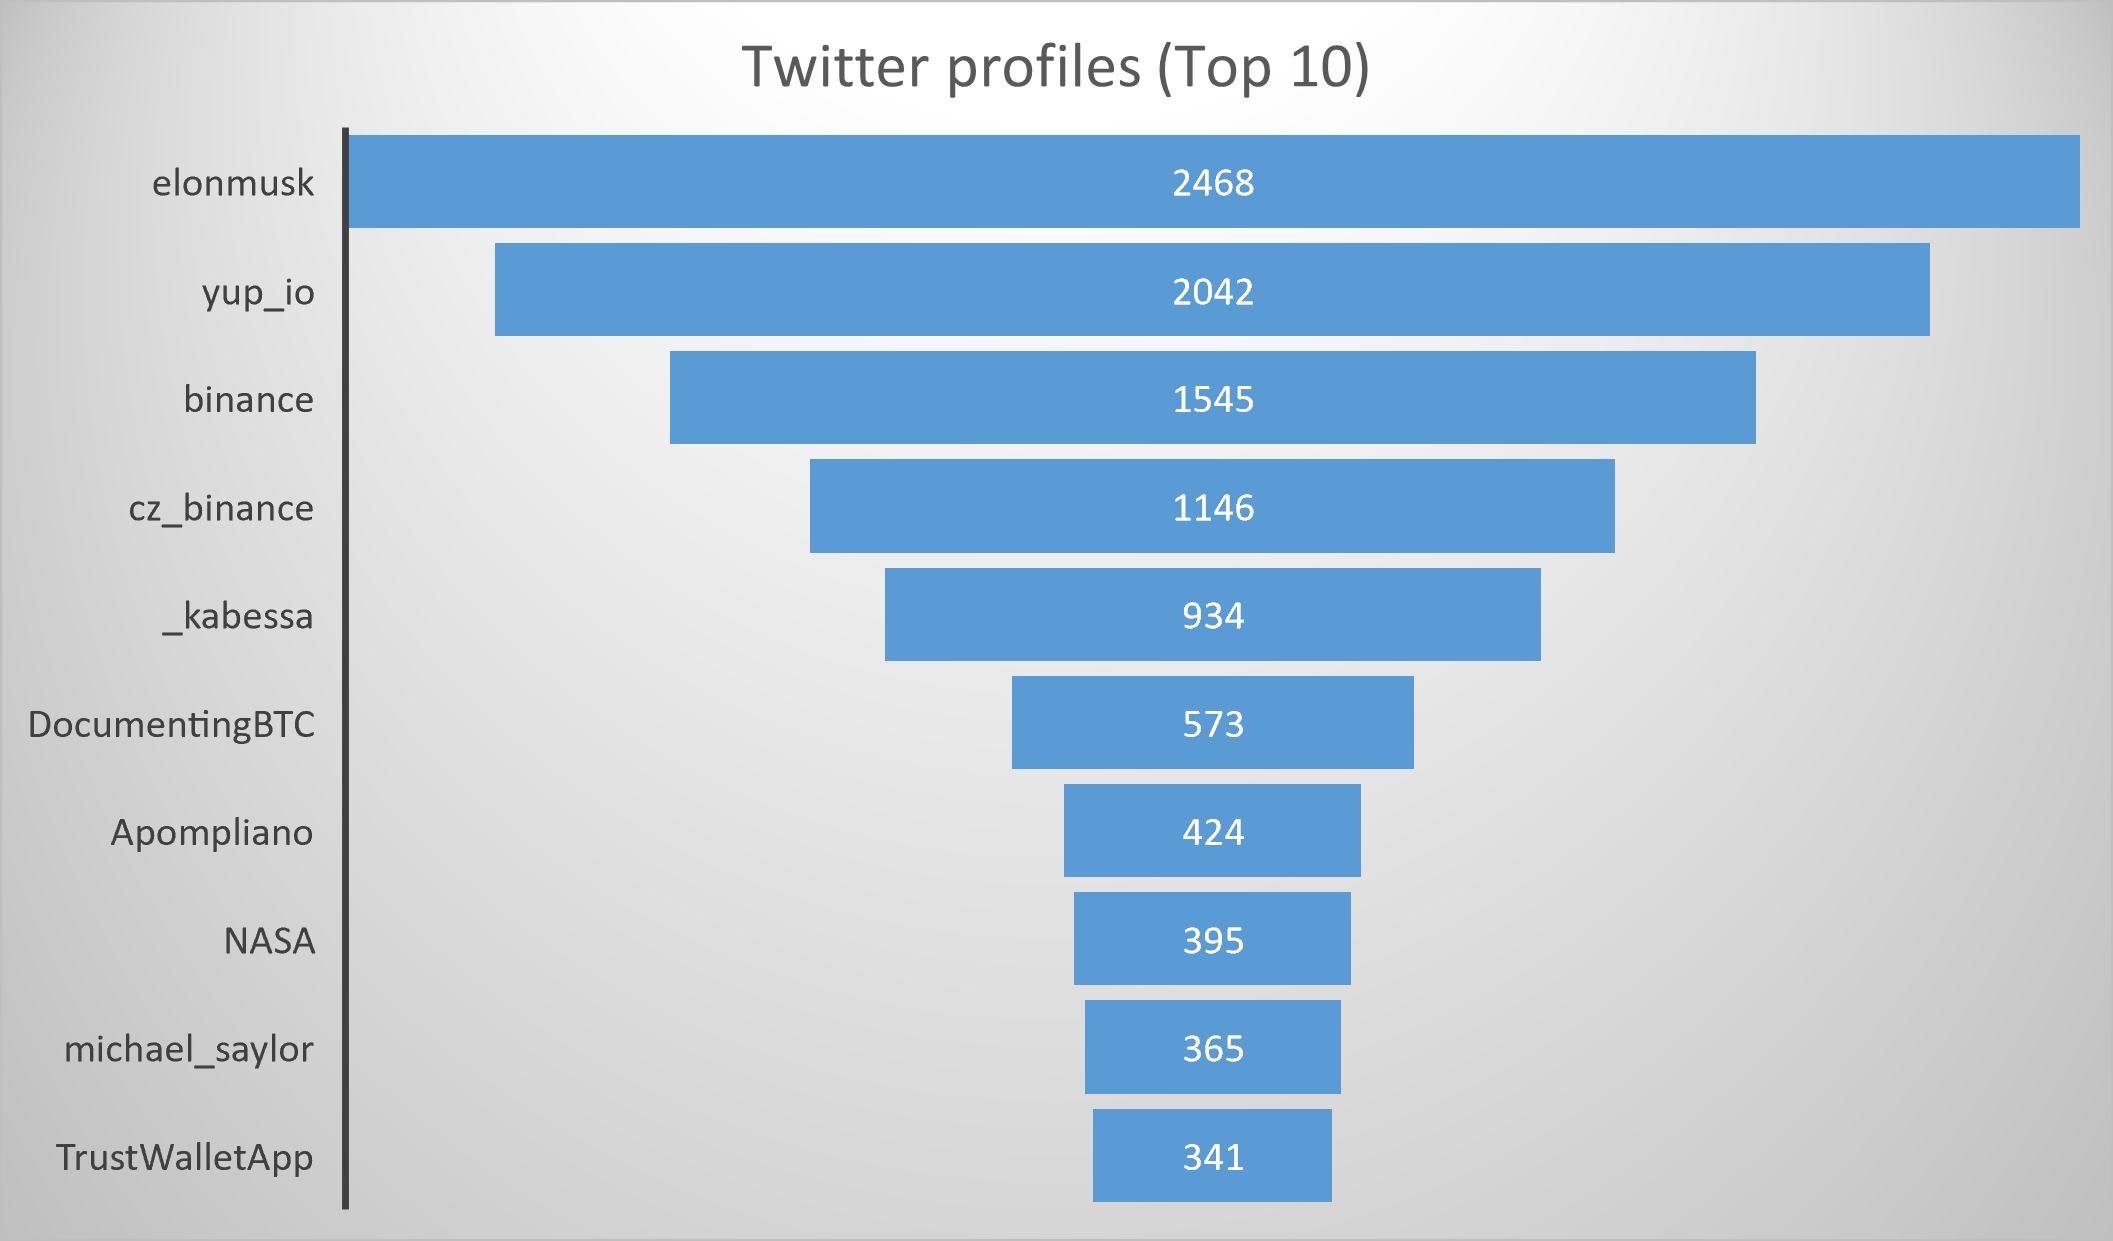
\includegraphics[width=0.8\textwidth]{graphs/twitter_profiles.png}
    \caption[twitter profiles]{Top 10 profili Twitter con più voti totali
    \\
    \centering
    \begin{itemize}
        \centering
        \item \textbf{VOTI TOTALI TWITTER:} 121.876
        \item \textbf{others:} 111.643
    \end{itemize}}
    \label{fig: twitter_profiles}
\end{figure}

Nel caso di Youtube è stato considerato un sottogruppo dei dati di partenza, abbiamo infatti tenuto conto dei soli video che avevano ricevuto più di un voto. Questo perché la quantità di voti era difficilmente trattabile, per via del limit rate imposto dalle API della piattaforma, necessarie per reperire il nome del canale Youtube partendo dal link del video votato. Inoltre aumentiamo la possibilità di escludere potenziali self-voters: questi non vengono infatti eliminati del tutto con il criterio utilizzato poiché, come già spiegato nel Capitolo \ref{platform_chapter}, è possibile effettuare fino a 3 voti sullo stesso contenuto cambiando la categoria.

\begin{figure}[t]
    \centering
    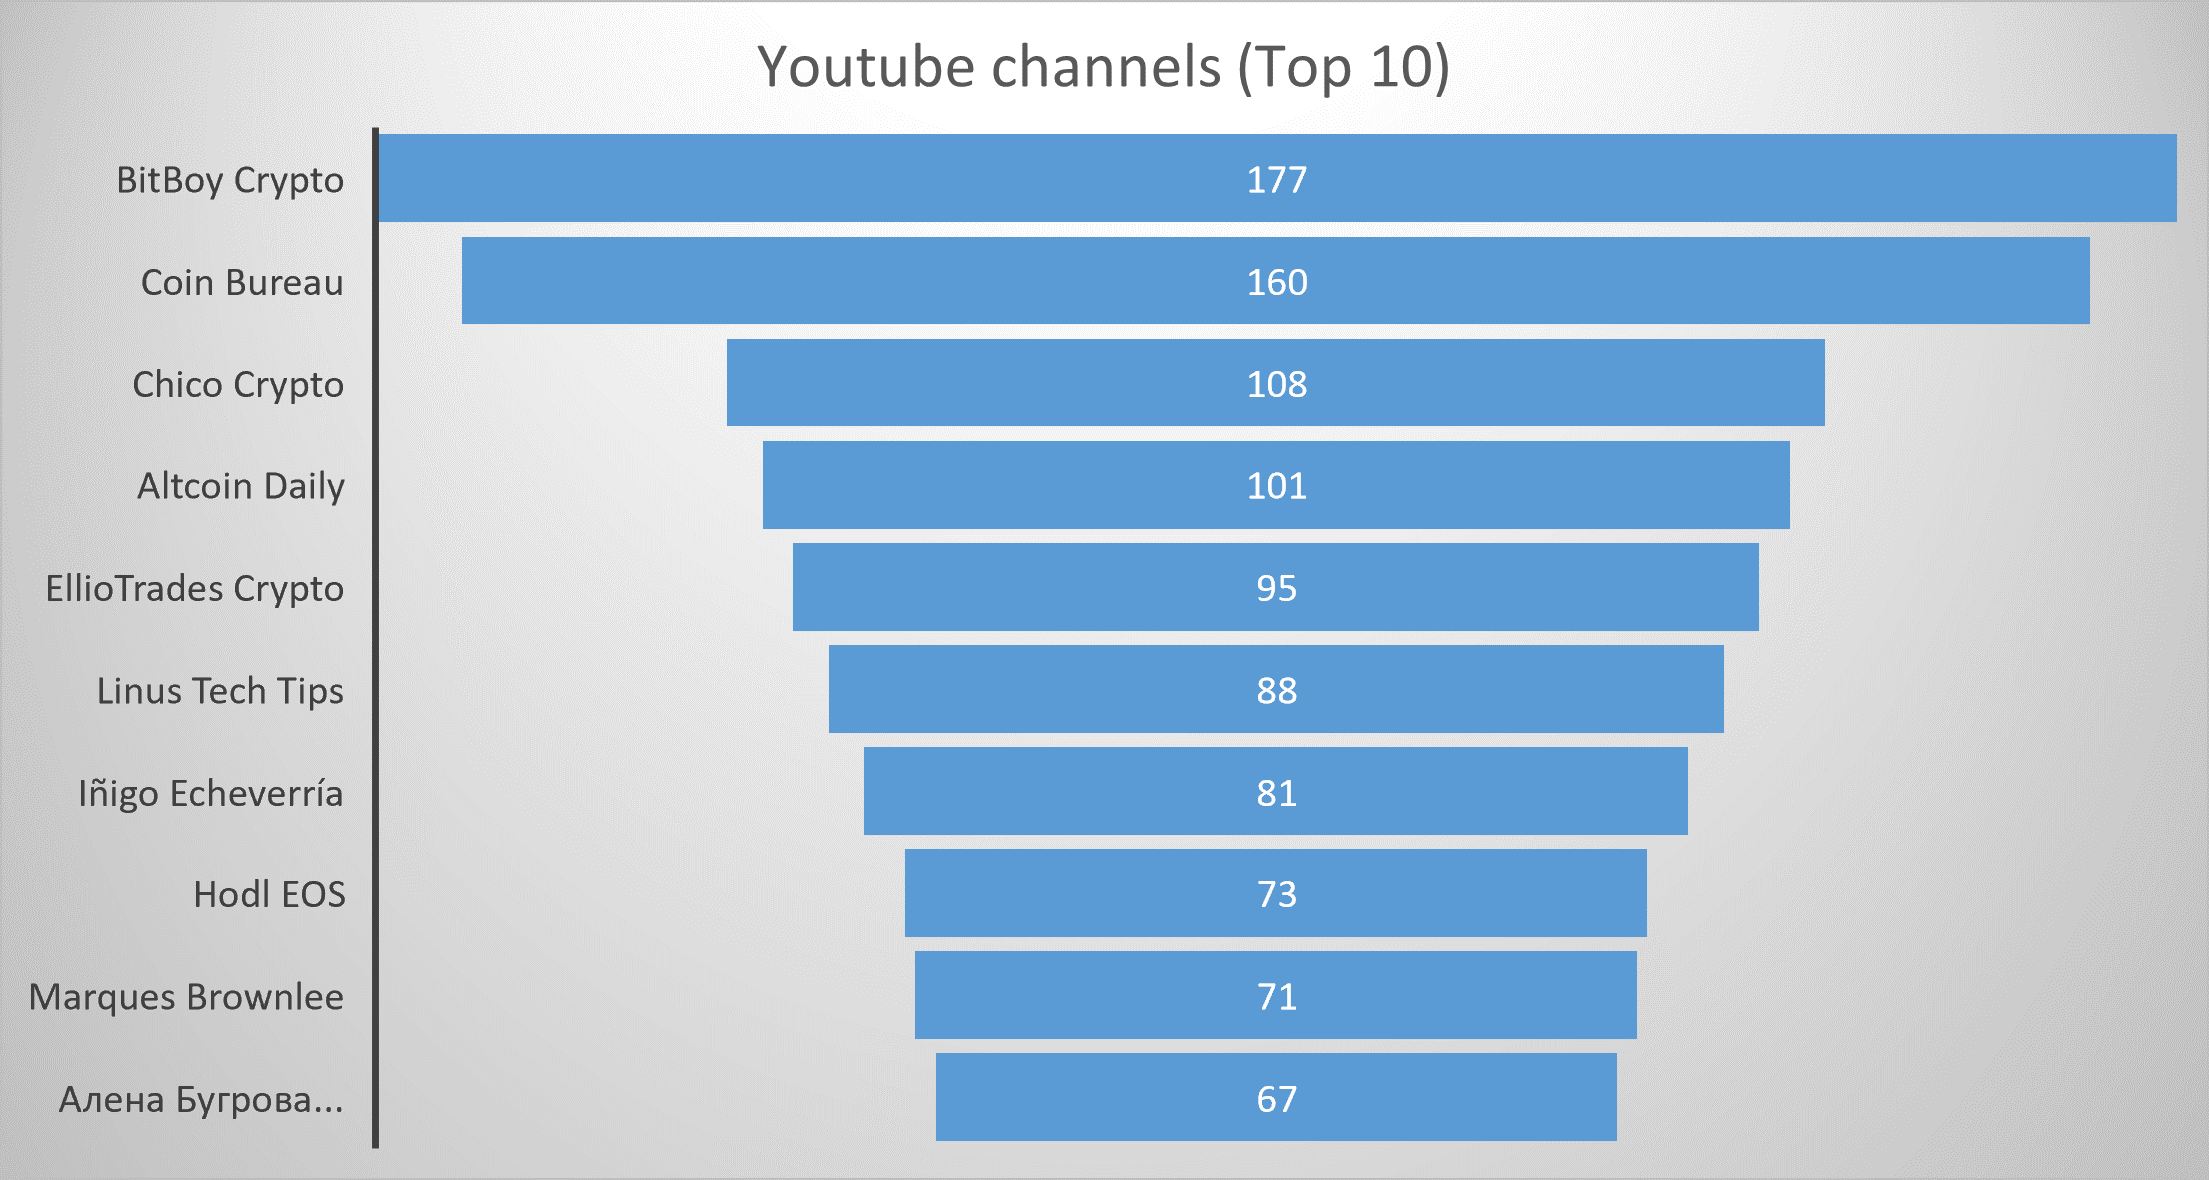
\includegraphics[width=0.7\textwidth]{graphs/youtube_channels.png}
    \caption[youtube channels]{Top 10 canali Youtube con più voti totali
    \\
    \centering
    \begin{itemize} \centering
        \item \textbf{VOTI TOTALI YOUTUBE:} 16.169
        \item \textbf{others:} 15.148
    \end{itemize}}
    \label{fig: youtube_channels}
\end{figure}

\begin{figure}[t]
    \centering
    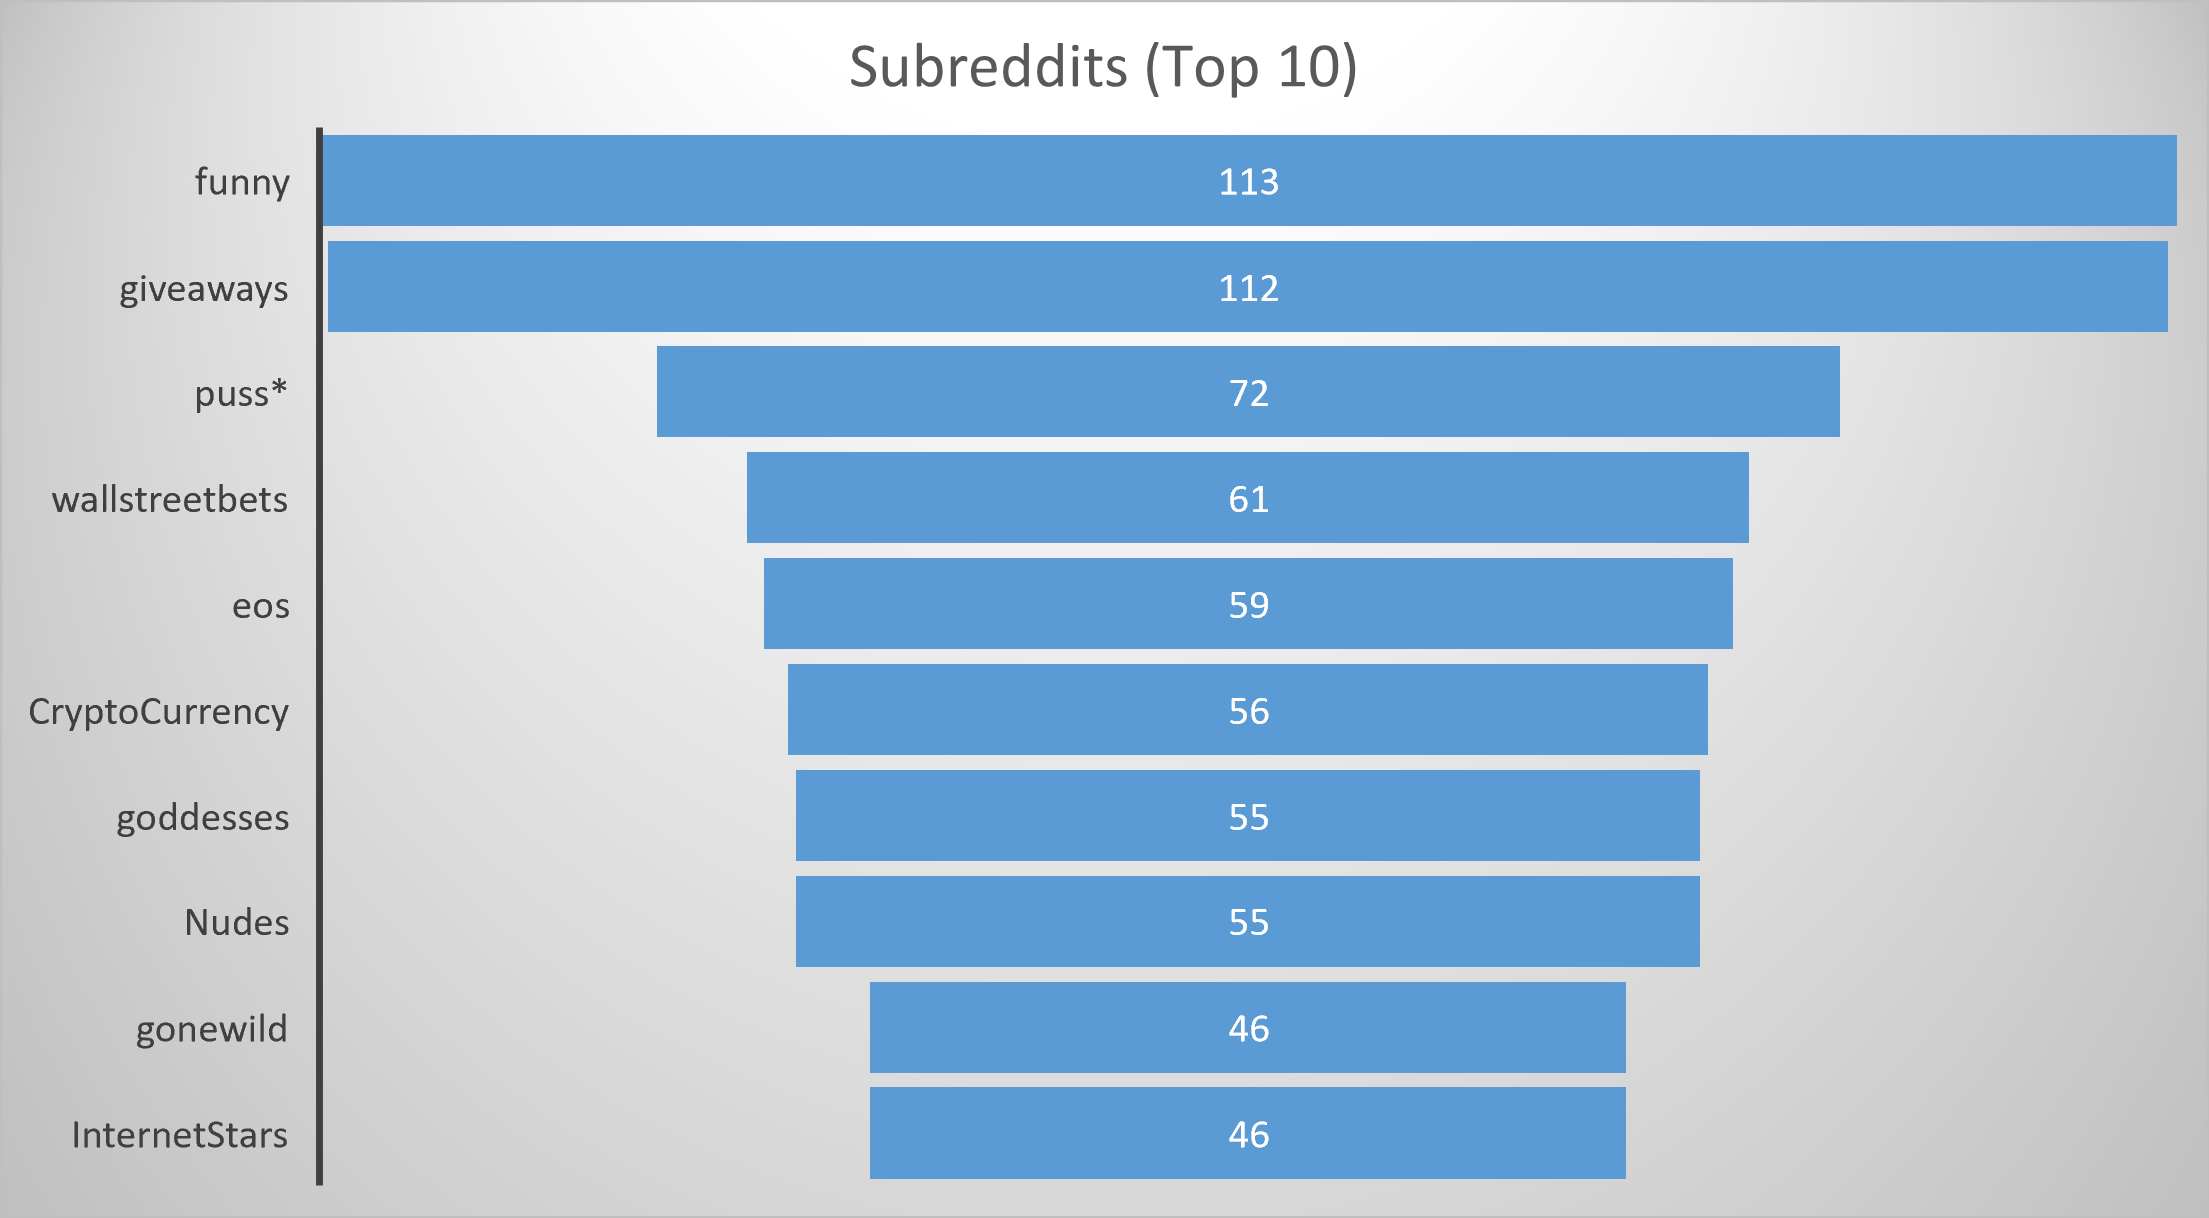
\includegraphics[width=0.7\textwidth]{graphs/subreddits.png}
    \caption[subreddits]{Top 10 subreddit di Reddit con più voti totali
    \\
    \centering
    \begin{itemize} \centering
        \item \textbf{VOTI TOTALI REDDIT:} 3.499
        \item \textbf{others:} 2.824
    \end{itemize}}
    \label{fig: reddit_subreddits}
\end{figure}


Osservando le 3 Figure, relative alle tre piattaforme più votate con Yup, il primo fatto che salta subito all'occhio è che la maggior parte dei voti venga attribuita ad individui o a gruppi che trattano o sono vicini al mondo cripto. 


Nel caso dei profili Twitter maggiormente votati è anche osservabile come siano presenti o individui di elevata notorietà in tale ambito (Elon Musk, CZ Binance, APompliano) o il profilo ufficiale di Yup (Yup.io) e quelli di alcuni developer (\_Kabessa).
Similmente, tra i canali Youtube più popolari troviamo quasi esclusivamente appassionati di criptovalute o altri canali dove si trattano argomenti tecnici legati alla tecnologia blockchain.
Su Reddit la situazione è più eterogenea, infatti troviamo subreddit legati a criptovalute (eos e CryptoCurrency), investimenti (wallstreetbets), ma anche alcuni subreddit con materiale NSFW (puss*, goddesses, Nudes, gonewild, InternetStars).

La forte attenzione riguardo al mondo delle criptovalute e delle blockchain in generale è un risultato atteso se, ricordando che le ricompense di un utente dipendono dal numero di voti che occorrono dopo il suo, pensiamo a come sia più probabile avere guadagni maggiori votando account molto seguiti o appartenenti a personaggi eccentrici, come Elon Musk, oppure anche account con meno seguaci ma la cui esposizione ad utenti Yup è intuitivamente significativa, come l'account ufficiale della dApp.
Questo ci porta inoltre a pensare che ci sia una certa polarizzazione nei contenuti maggiormente monitorati dagli utenti.
Questo fenomeno potrebbe ulteriormente amplificarsi nel tempo.
Infatti se i nuovi utenti saranno solamente interessati a generare profitto, la loro migliore strategia per generarne il più possibile sarebbe quella di sfruttare l'estrema popolarità di questi account ed esprimere un voto il prima possibile, andando ad invalidare le premesse della piattaforma.
D'altro canto questo risultato, unito a quello della distribuzione dei voti per piattaforma, potrebbe essere invece segnale che l'utenza che utilizza il servizio, almeno per il momento, sia prevalentemente di nicchia.
Un risultato naturale se si pensa che sia più probabile che persone interessate a questi argomenti abbiano sentito parlare di Yup e di conseguenza si siano iscritti. 


\subsection{Distribuzione utenti-piattaforme}
Ci siamo infine concentrati sulla possibilità che un utente possieda o meno un account su altri social network. Ricordiamo infatti che su ogni piattaforma, anche se non integrata sull'applicazione ufficiale di Yup, è possibile esprimere la valutazione di un contenuto e registrare la valutazione sullo smart contract EOS d Yup. Nel nostro studio abbiamo selezionato solo alcune piattaforme tra quelle più famose anche non nel mondo cripto: Twitter, Youtube, Facebook, Reddit, Instagram, Spotify. Di seguito indichiamo, per ognuna di queste piattaforme, il numero di utenti che ne hanno votato almeno un contenuto:

\begin{itemize}
    \item \textbf{TWITTER}: 2.272
    \item \textbf{YOUTUBE}: 2.379
    \item \textbf{REDDIT}: 307
    \item \textbf{FACEBOOK}: 80
    \item \textbf{INSTAGRAM}: 39
    \item \textbf{SPOTIFY}: 44
\end{itemize}

Twitter e Youtube si confermano le piattaforme social più popolari dal punto di vitsta della votazione, ma notiamo che il numero di utenti che ha votato almeno un contenuto Youtube è leggermente superiore al numero di utenti che ha votato almeno un contenuto su Twitter.
Se consideriamo che il numero di voti espressi su Twitter (Figura \ref{fig: twitter_profiles}) è circa 7.5 volte il numero di voti espressi su Youtube (Figura \ref{fig: youtube_channels}), possiamo anche concludere che spesso su Youtube si esprimono pochi voti.

Partendo da questi dati abbiamo anche effettuato un'intersezione tra gli insiemi di utenti che hanno votato le piattaforme considerate, ottenendo un totale di \textbf{3.232 votatori unici} (sono 5.121 gli utenti che hanno espresso almeno un voto). Riportiamo la distribuzione del numero di utenti per il numero di piattaforme votate:

\begin{itemize}
    \item \textbf{6/6}: 4
    \item \textbf{5/6}: 12
    \item \textbf{4/6}: 42
    \item \textbf{3/6}: 254
    \item \textbf{2/6}: 1.187
    \item \textbf{1/6}: 1.733
\end{itemize}

Questa distribuzione ci suggerisce che sono pochi gli utenti che utilizzano Yup al pieno del suo potenziale e che in genere si preferisce concentrarsi su al più due piattaforme. 

Da questo studio tuttavia non si ha la certezza che un individuo possieda un account su una determinata piattaforma, anche nel caso in cui per visualizzare un contenuto e quindi votarlo sia necessario il login (per esempio su \textbf{Instagram} o \textbf{Facebook}).
Questo succede perché, tramite l'interfaccia di Yup.io, è possibile esprimere opinioni in maniera "indiretta", ispezionando l'attività di altri utenti. Per esempio un utente può votare un contenuto relativo a Facebook che è stato votato da un altro utente accedendo al suo profilo e votandolo sulla piattaforma.


Con l'idea di ottenere risultati più accurati riguardo il fatto di possedere un account su una delle piattaforme studiate, è stata ripetuta la stessa analisi considerando solo gli utenti che sono stati i primi a votare (studiando quindi le azioni della famiglia postvote).
Grazie a questa analisi, almeno per quelle piattaforme in cui il login è obbligatorio, (Youtube, Reddit, e Twitter sono fanno eccezione ma riportiamo comunque i loro dati per completezza), il voto è stato necessariamente effettuato in maniera "diretta", ovvero visualizzando il contenuto sulla piattaforma social e votando tramite overlay Yup, e quindi il votatore deve esservi registrato.

\begin{itemize}
    \item \textbf{TWITTER}: 1.402
    \item \textbf{YOUTUBE}: 1.109
    \item \textbf{REDDIT}: 187
    \item \textbf{FACEBOOK}: 43
    \item \textbf{INSTAGRAM}: 26
    \item \textbf{SPOTIFY}: 21
\end{itemize}

%Categorie: spostata in YupPlatform

%Account Mirror: spostata sopra in trattazione figure dei solo Mirror

\section{Utilizzo del Bridge}
Passiamo ora allo studio del bridge, ovvero la componente che serve per gestire il flusso di criptovaluta e l'interazione tra le blockchain di EOS e Ethereum.
Di seguito riportiamo un'analisi che ha l'obiettivo, considerando esclusivamente i trasferimenti di token verso Ethereum (quindi un "prelievo" di YUP) e quelli relativi al pagamento delle corrispondenti tasse, di dare un'idea di quanto nell'utenza abbia guadagnato tramite l'utilizzo del servizio e di quanto abbia perso per via delle tasse legate al Bridge. Abbiamo escluso quei trasferimenti effettuati da \textbf{yupaccounts1} e \textbf{testpoolbox1} poiché transazioni atte a testare il Bridge al momento della sua introduzione, di fatto hanno effettuato i primi trasferimenti e non compaiono più successivamente.


Le azioni che si occupano del trasferimento dei token verso l'indirizzo Ethereum dell'utente (riportato nel campo \textbf{memo} dell'azione) hanno come destinatario dell'azione EOS \textbf{bridge.yup}. Questo perché viene adottato un approccio \textbf{mint-burn} (descritto nell'apposita sezione Bridge nel \textbf{Capitolo 3}), ovvero i token non vengono realmente spostati dalla blockchain, ma vengono "bruciati" su EOS e creati su Ethereum. Mostriamo in Tabella \ref{tab: bridge_analytics} alcuni dati di analisi tenendo in considerazione solo i transfer verso indirizzi Ethereum e in Figura \ref{fig: top10_bridge} gli utenti che hanno spostato la maggior quantità di token.


\begin{table}[h]
\centering
\begin{tabular}{ |c|c|}
 \hline
 TRASFERIMENTI DI TOKEN SU ETH & 334 \\
 \hline
 TOKEN MIGRATI SU ETH & 119.024,47 YUP \\
 \hline
 MASSIMO BRIDGE & 24.950 YUP \\
 \hline
 MINIMO BRIDGE & 0,001 YUP \\
 \hline
 MEDIA BRIDGE & 356,36 YUP \\
 \hline
\end{tabular}
\caption{Dati analitici dell'utilizzo del Bridge}
\label{tab: bridge_analytics}
\end{table}

La Tabella ci mostra che l'utilizzo del bridge è limitato a poche centinaia di transazioni, e quindi poco comune su Yup se comparato al altre attività, come il voto.
Ciononostante, notiamo che oltre 100.000 token sono stati trasferiti da EOS a Ethereum, probabilmente perché Ethereum ospita molte dapp e il mercato di compravendita di token su Ethereum è molto più florido, rendendo quindi i token più facilmente scambiabili.

\begin{figure}[t]
    \centering
    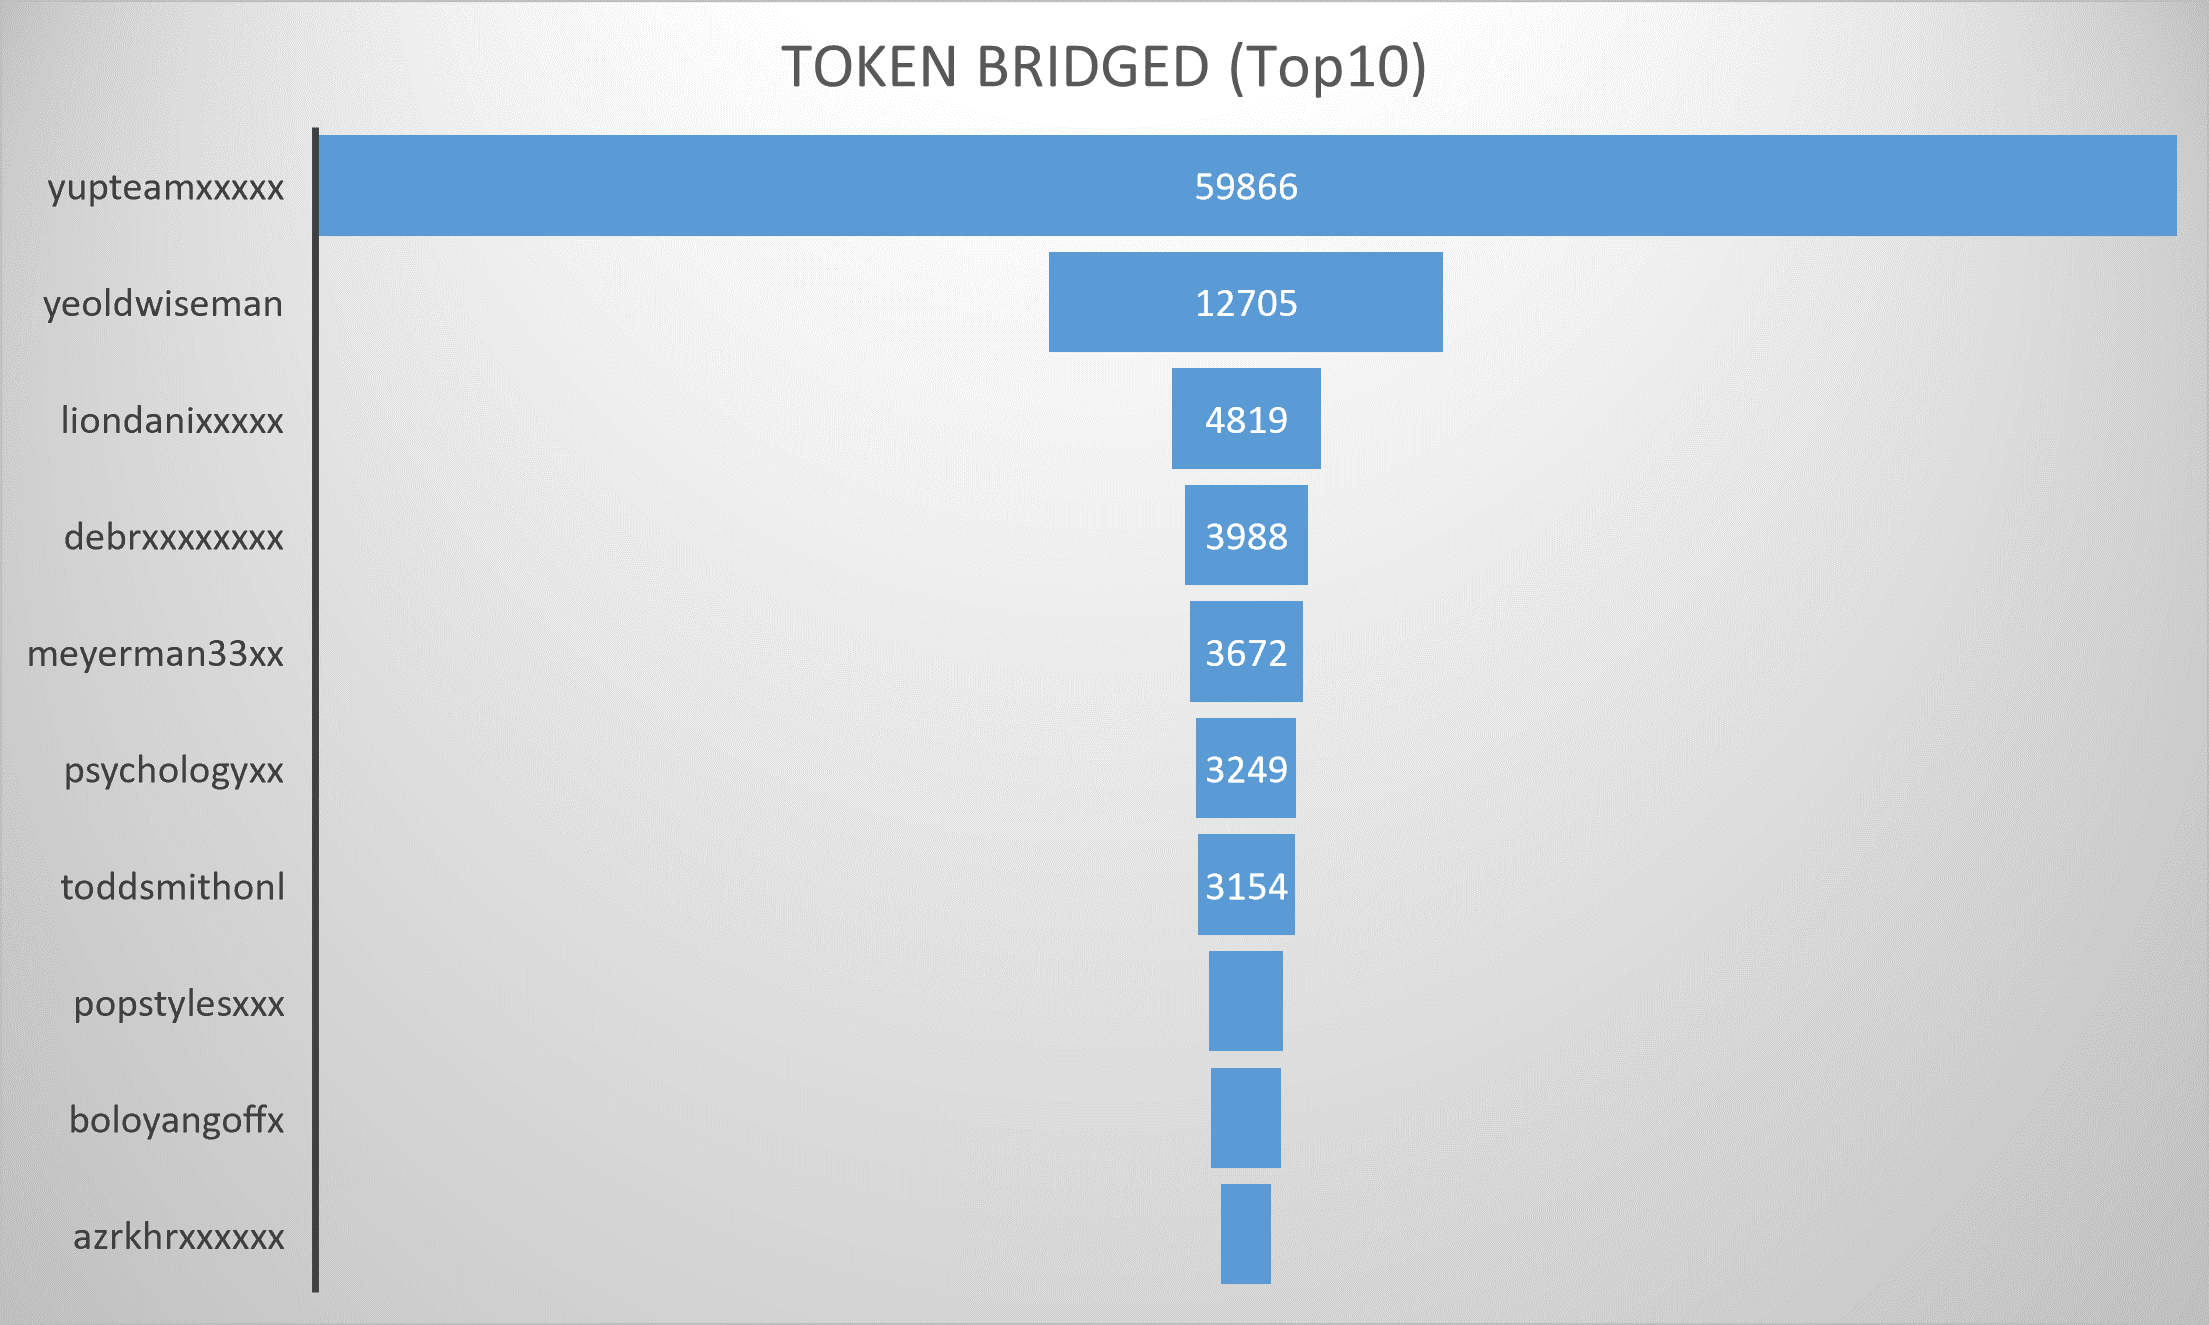
\includegraphics[width=.7\textwidth]{graphs/top10_bridge.png}
    \caption{Top 10 degli account che hanno trasferito la maggior quantità di token su Ethereum}
    \label{fig: top10_bridge}
\end{figure}

Dalla Figura possiamo invece osservare come l'account \textit{yupteamxxxxx} sia di gran lunga quello ad aver migrato più token sulla blockchain di Ethereum (Figura \ref{fig: top10_bridge}). Quest'ultimo raggruppa tutte le ricompense che, secondo quanto descritto nella documentazione della piattaforma, sono destinate ai membri del team.

Le azioni che si occupano del trasferimento dei token in qualità di tassa sono invece rivolte verso \textbf{yupaccounts1}. Mostriamo in Tabella \ref{tab: fees_analytics} alcuni dati di analisi tenendo in considerazione solo i transfer in quanto pagamento della tassa del Bridge e in Figura \ref{fig: top10_fees} gli utenti che hanno "speso" la maggior quantità di token per via della tassa sul trasferimento all'account bridge.

\begin{table}[h!]
\centering
\begin{tabular}{ |c|c|}
 \hline
 TRASFERIMENTI DI TASSE & 333 \\
 \hline
 TOKEN PERSI IN TASSE & 2.781,79 YUP \\
 \hline
 MASSIMA TASSA PAGATA & 62,45 YUP \\
 \hline
 MINIMA TASSA PAGATA & 0,18 YUP \\
 \hline
 MEDIA TASSA & 8,35 YUP \\
 \hline
\end{tabular}
\caption{Dati analitici delle tasse del Bridge}
\label{tab: fees_analytics}
\end{table}

\begin{figure}[t]
    \centering
    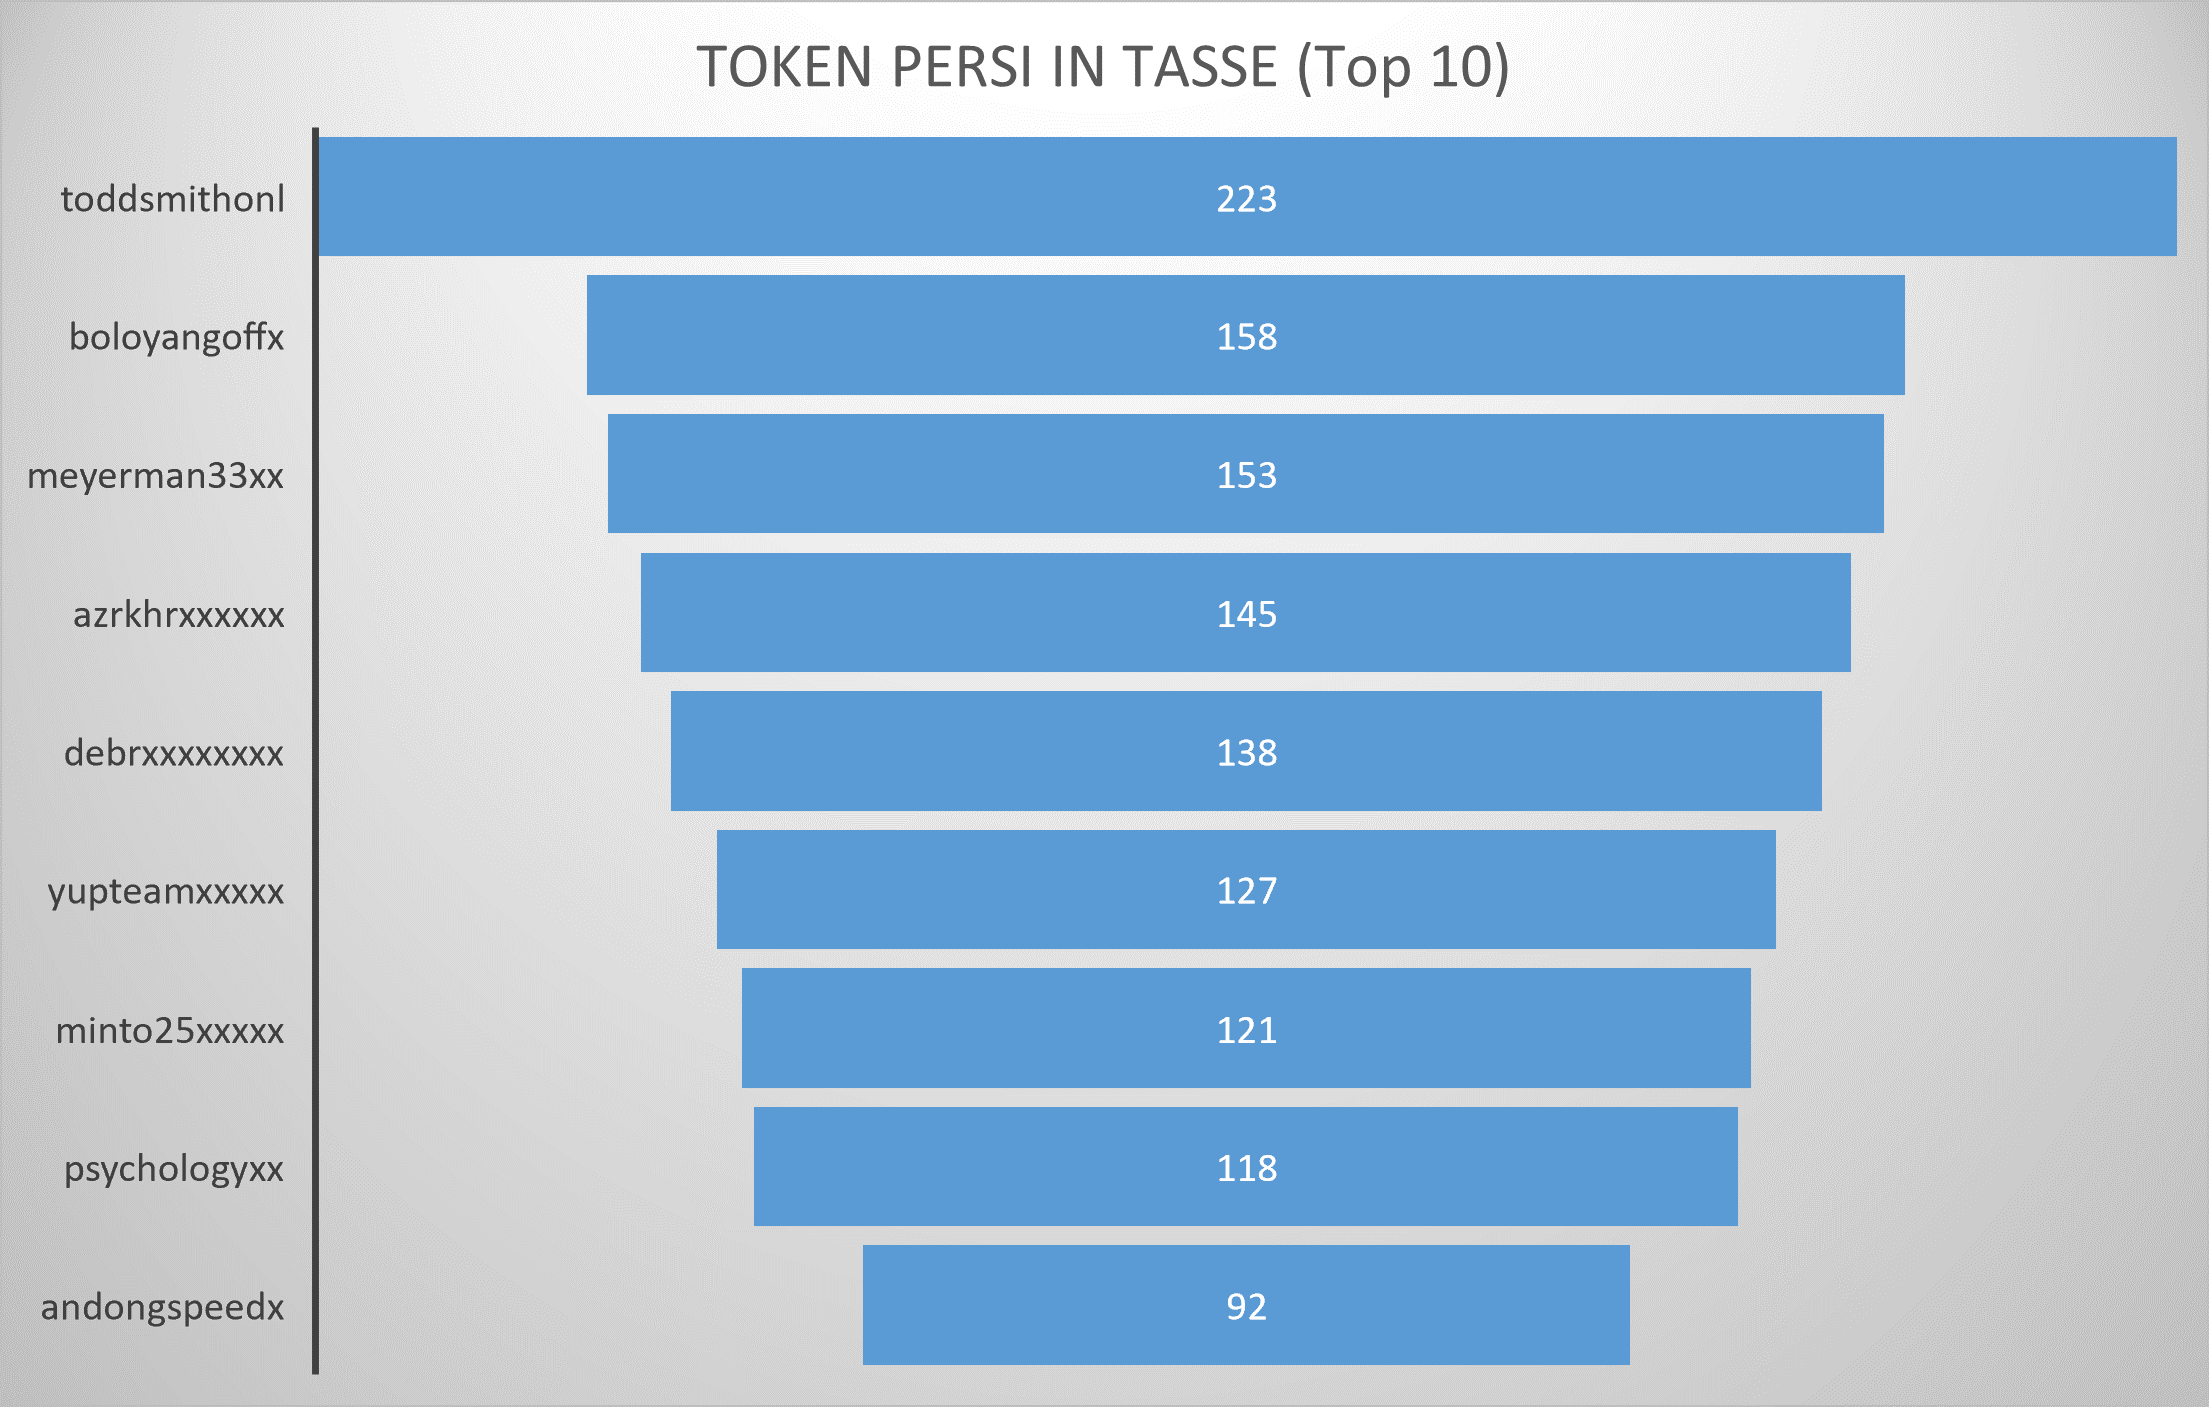
\includegraphics[width=.7\textwidth]{graphs/top10_fees.png}
    \caption{Top 10 degli account che hanno perso la maggior quantità di token in tasse}
    \label{fig: top10_fees}
\end{figure}

Notiamo come il numero dei bridge e quello dei pagamenti tasse differisca di uno. L'ipotesi è che questo sia stato effettuato in un periodo in cui la commissione fosse equivalente a 0, anche se è possibile si tratti semplicemente di un bug.

In conclusione possiamo affermare come ci sia un utilizzo del servizio del Bridge generalmente ristretto a pochi utenti, ma che è in grado di spostare ingenti somme di token.
Uno dei motivi che potrebbe ostacolare un più largo utilizzo di questo sistema è sicuramente legato al fatto che effettuare un trasferimento di token su Ethereum comporta il pagamento di una commissione. 

\section{Distribuzione Token}

\begin{figure}[t]
    \centering
    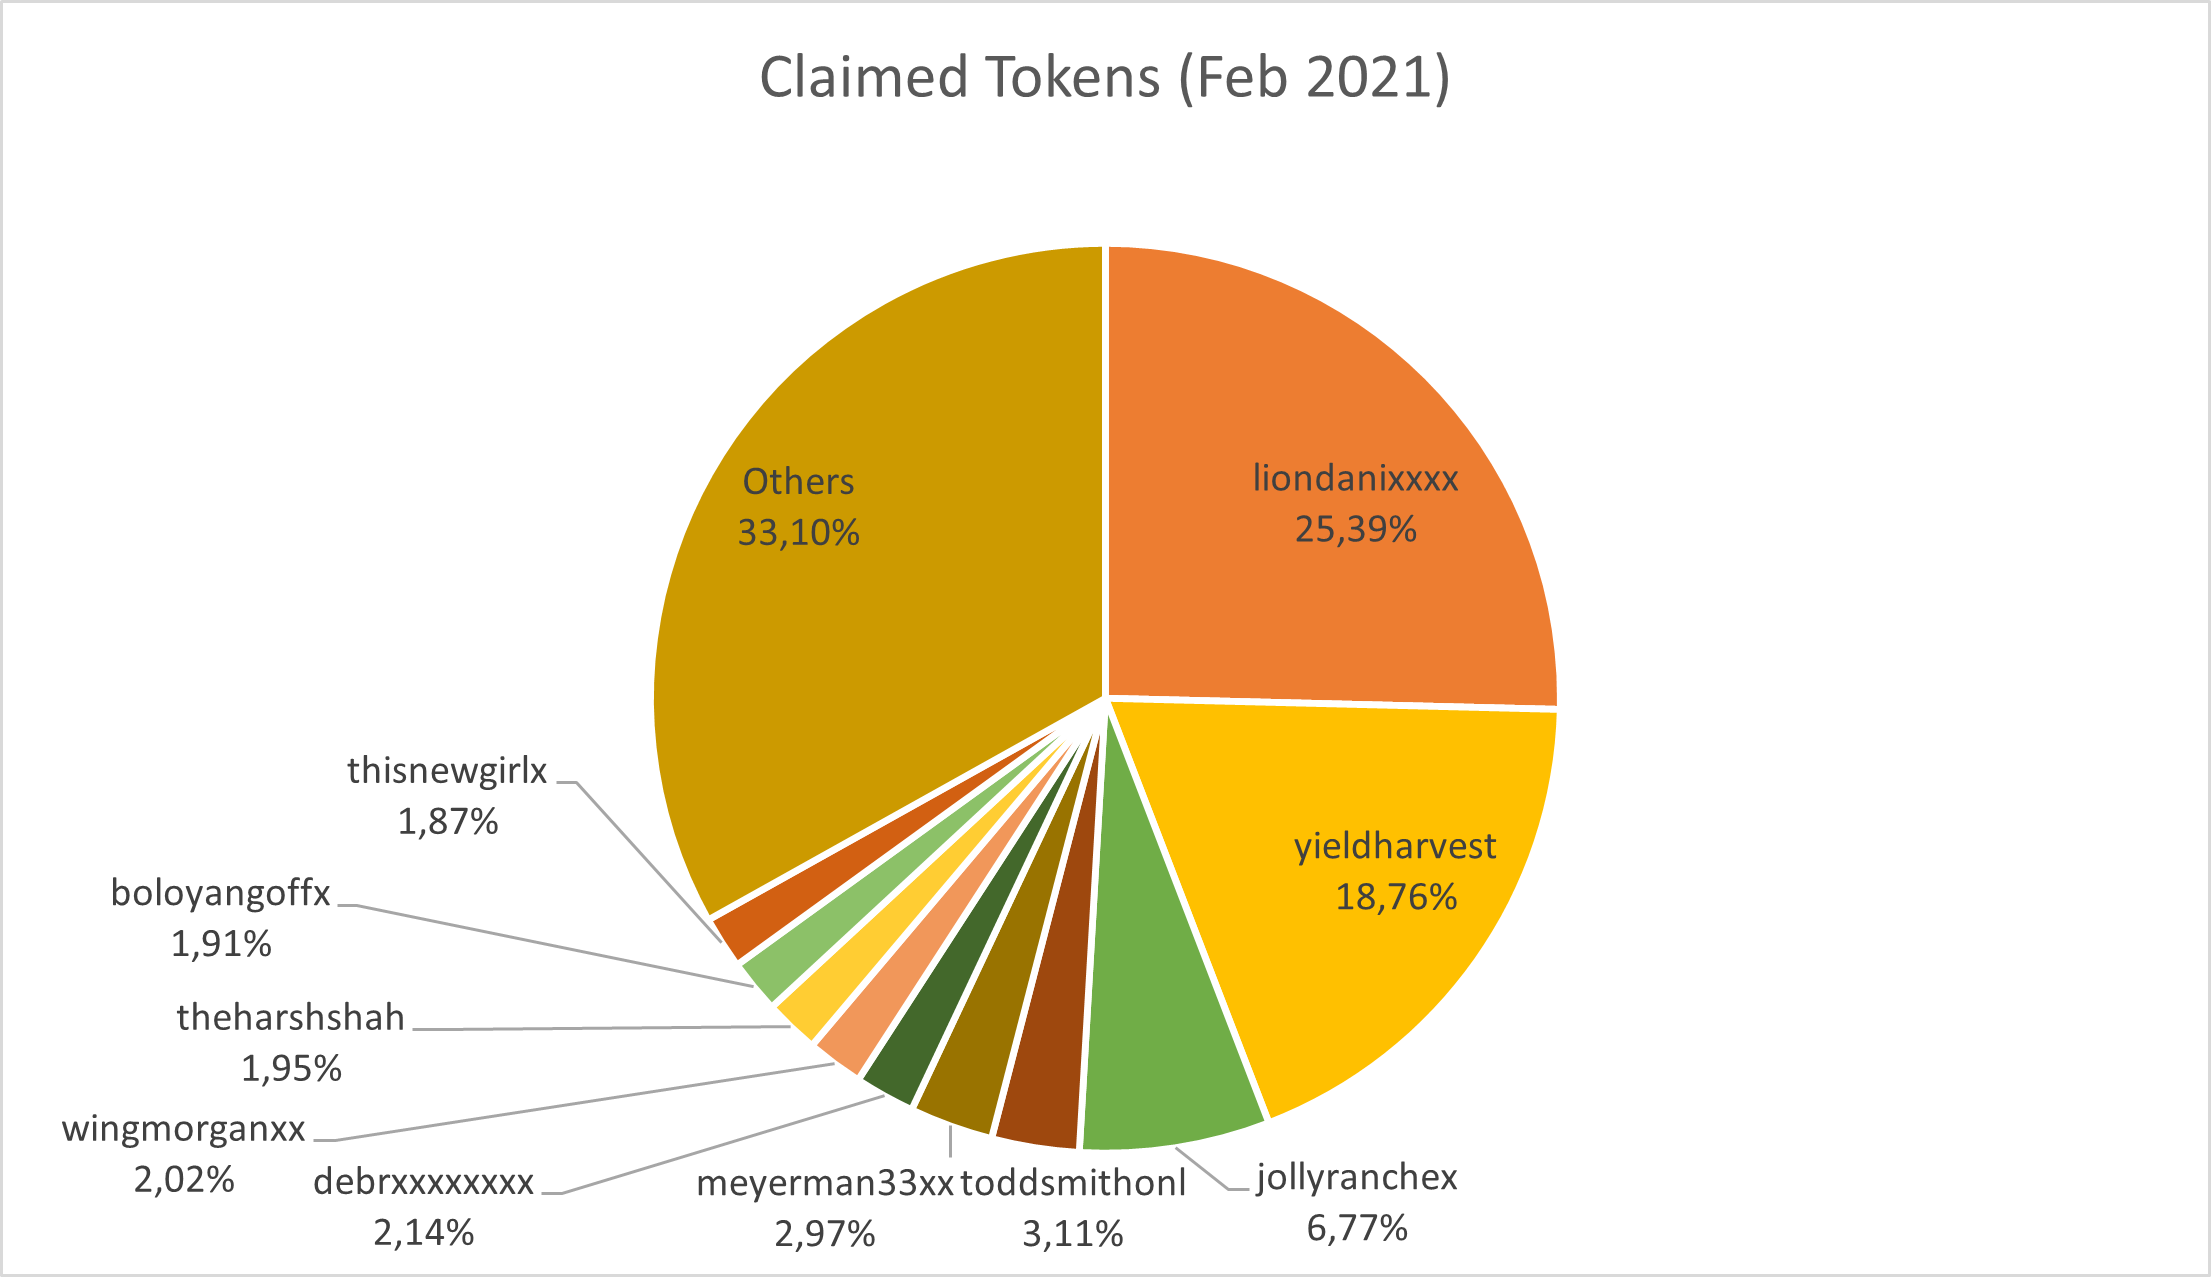
\includegraphics[width=1\textwidth]{graphs/token_claimed_february.png}
    \caption{Top 10 degli utenti che hanno guadagnato più token fino a Febbraio 2021. In \textbf{others} sono inclusi tutti gli utenti restanti.}
    \label{fig: tokens_claimed_feb}
\end{figure}    
    %\vspace*{\floatstep}
\begin{figure}[t]
    \centering
    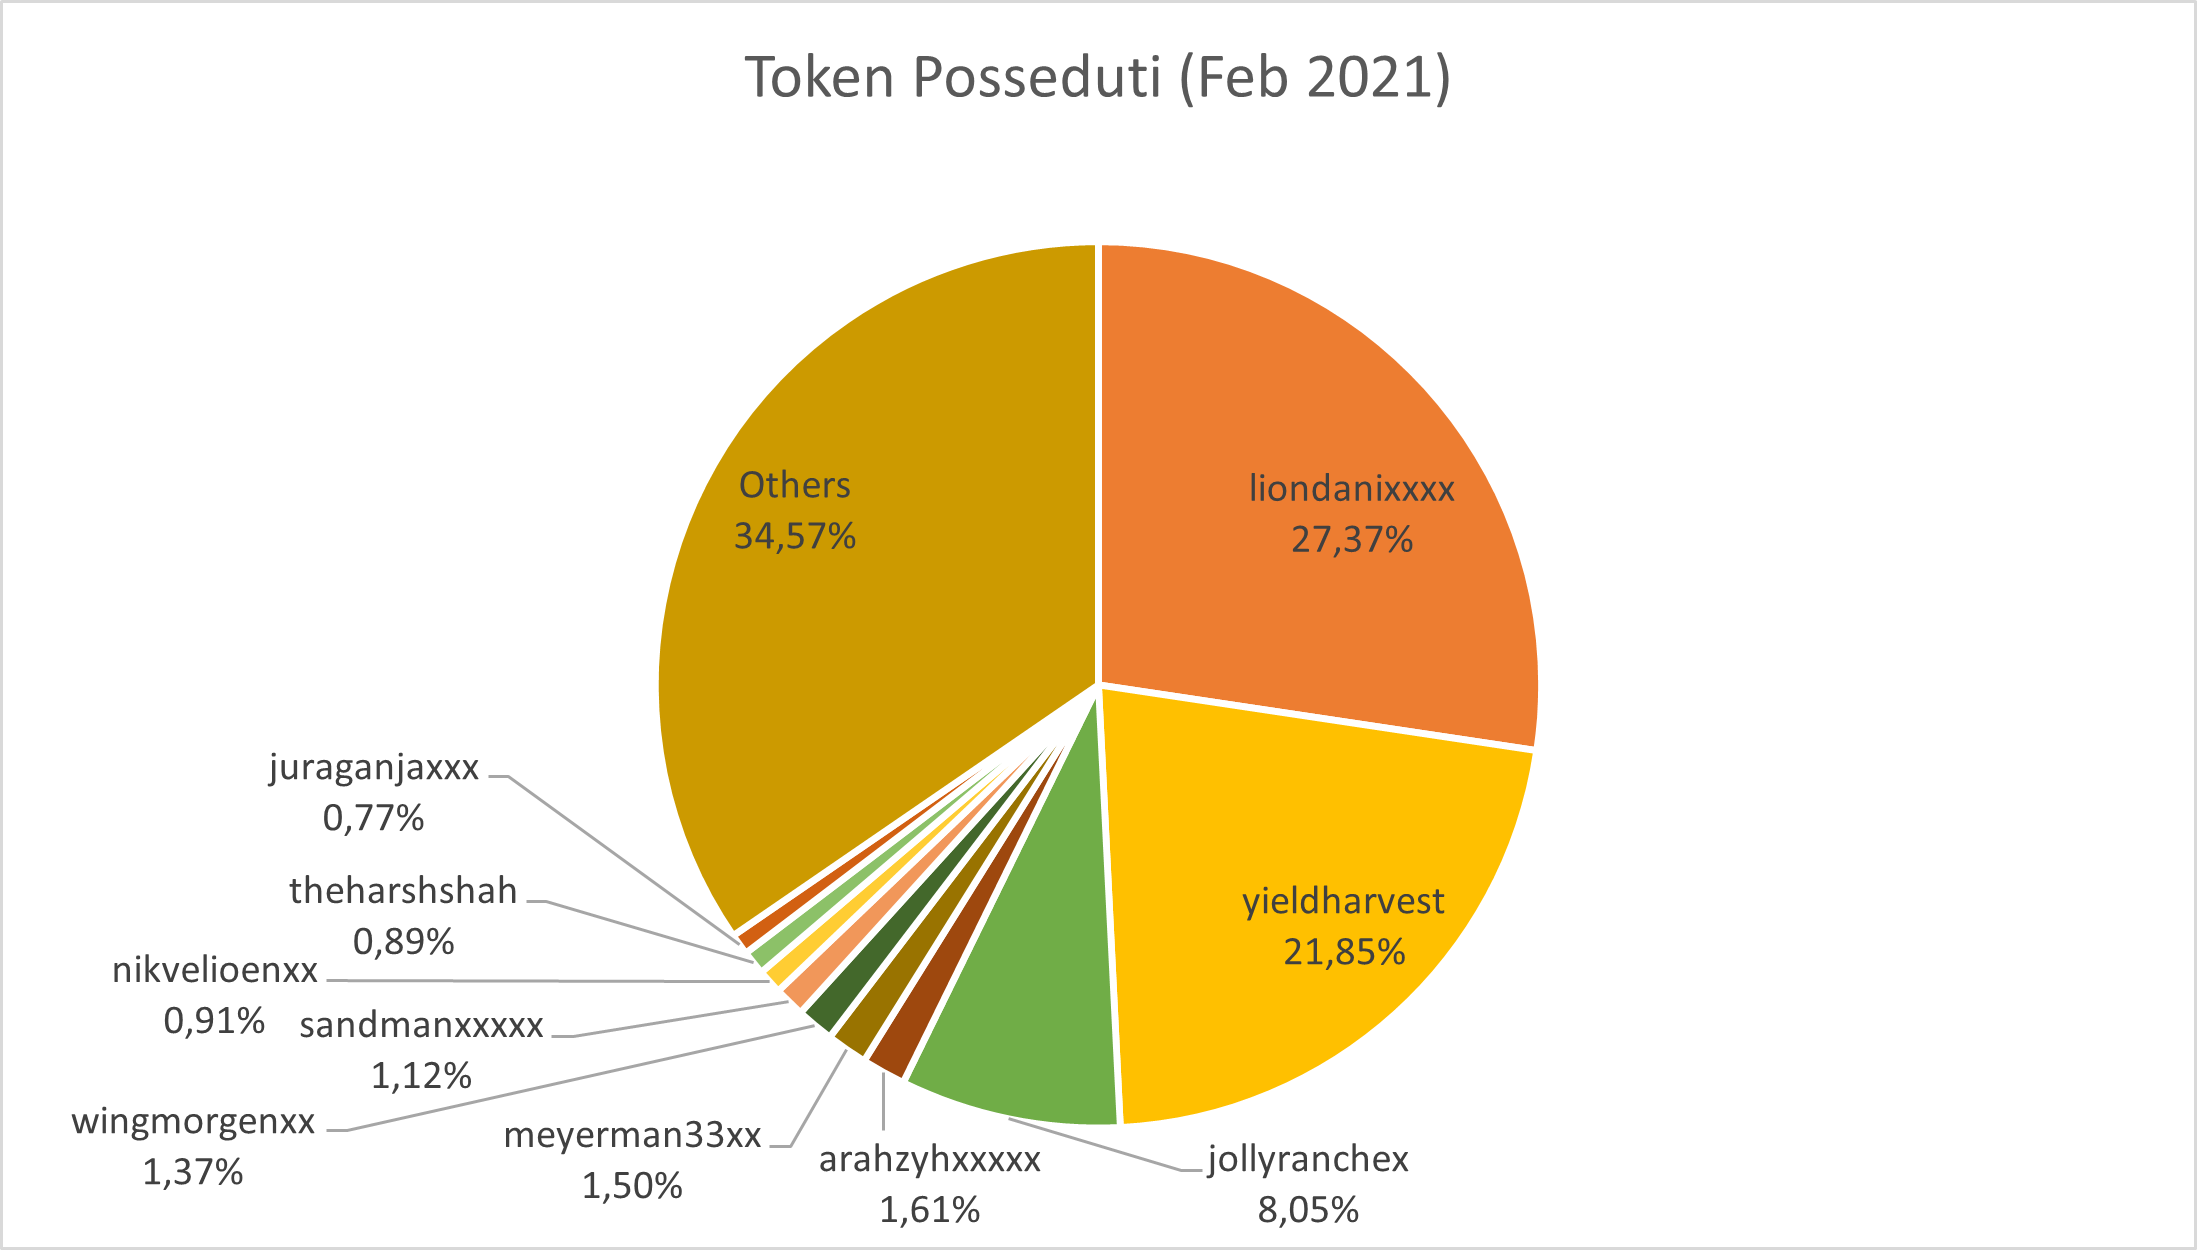
\includegraphics[width=1\textwidth]{graphs/token_posseduti_february.png}
    \caption{Top 10 degli utenti che possiedono più token a Febbraio 2021. In \textbf{others} sono inclusi tutti gli utenti restanti.}
    \label{fig: tokens_hold_feb}
\end{figure}

L'ultimo oggetto delle nostre analisi è quello dello studio in generale della distribuzione dei token tra gli utenti Yup. In particolare abbiamo deciso di concentrarci sugli account che hanno guadagnato di più e su quelli che possiedono attualmente più token.

Dopo esserci fatti un'idea dell'utilizzo di Bridge e della quantità di token migrati su Ethereum o persi in tasse, vedremo gli utenti che hanno ottenuto più ricompense e che possedevano più token nel mese di Febbraio 2021 (rispettivamente Figura \ref{fig: tokens_claimed_feb} e \ref{fig: tokens_hold_feb}) e in quello di Marzo 2021 (rispettivamente Figura \ref{fig: tokens_claimed_march} e \ref{fig: tokens_hold_march}.
Precisiamo che i token "claimed", cioè ottenuti tramite l'assegnazione delle ricompense, non indicano per forza quelli di cui l'utente è ancora in possesso poiché i token possono essere trasferiti ad altri utenti Yup, come mance sotto forma di azioni transfer, o su un suo wallet Ethereum, tramite il Bridge.


\begin{figure}[t]
    \centering
    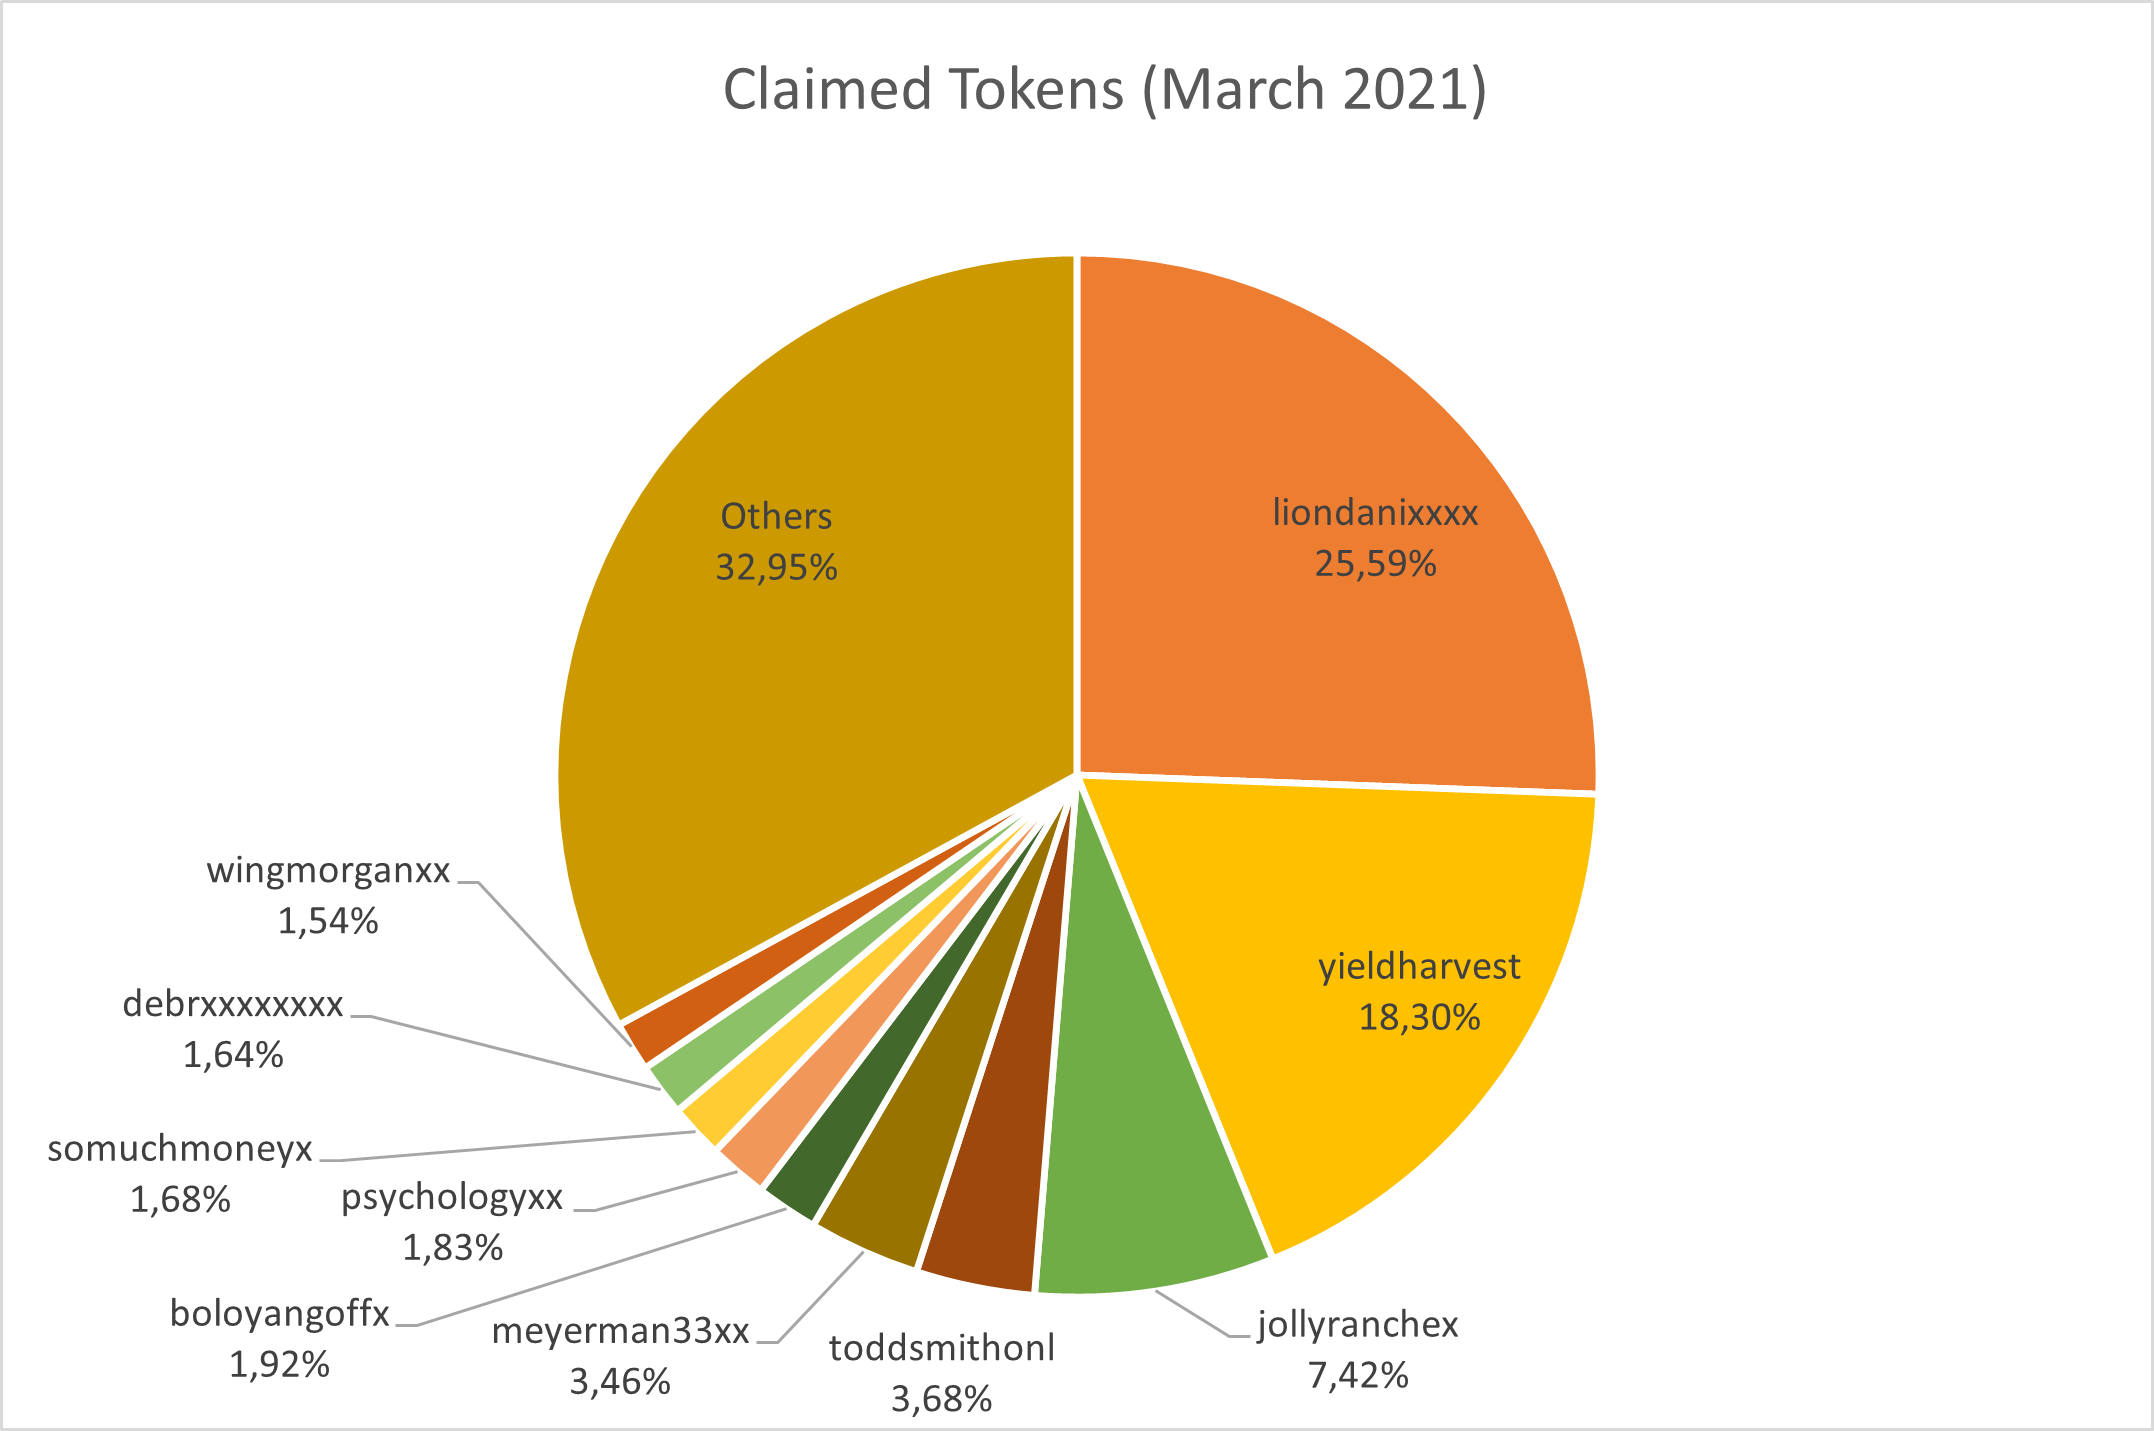
\includegraphics[width=1\textwidth]{graphs/token_claimed_march.png}
    \caption{Top 10 degli utenti che hanno guadagnato più token fino a Marzo 2021. In \textbf{others} sono inclusi tutti gli utenti restanti.}
    \label{fig: tokens_claimed_march}
\end{figure}    
    %\vspace*{\floatstep}
\begin{figure}[t]
    \centering
    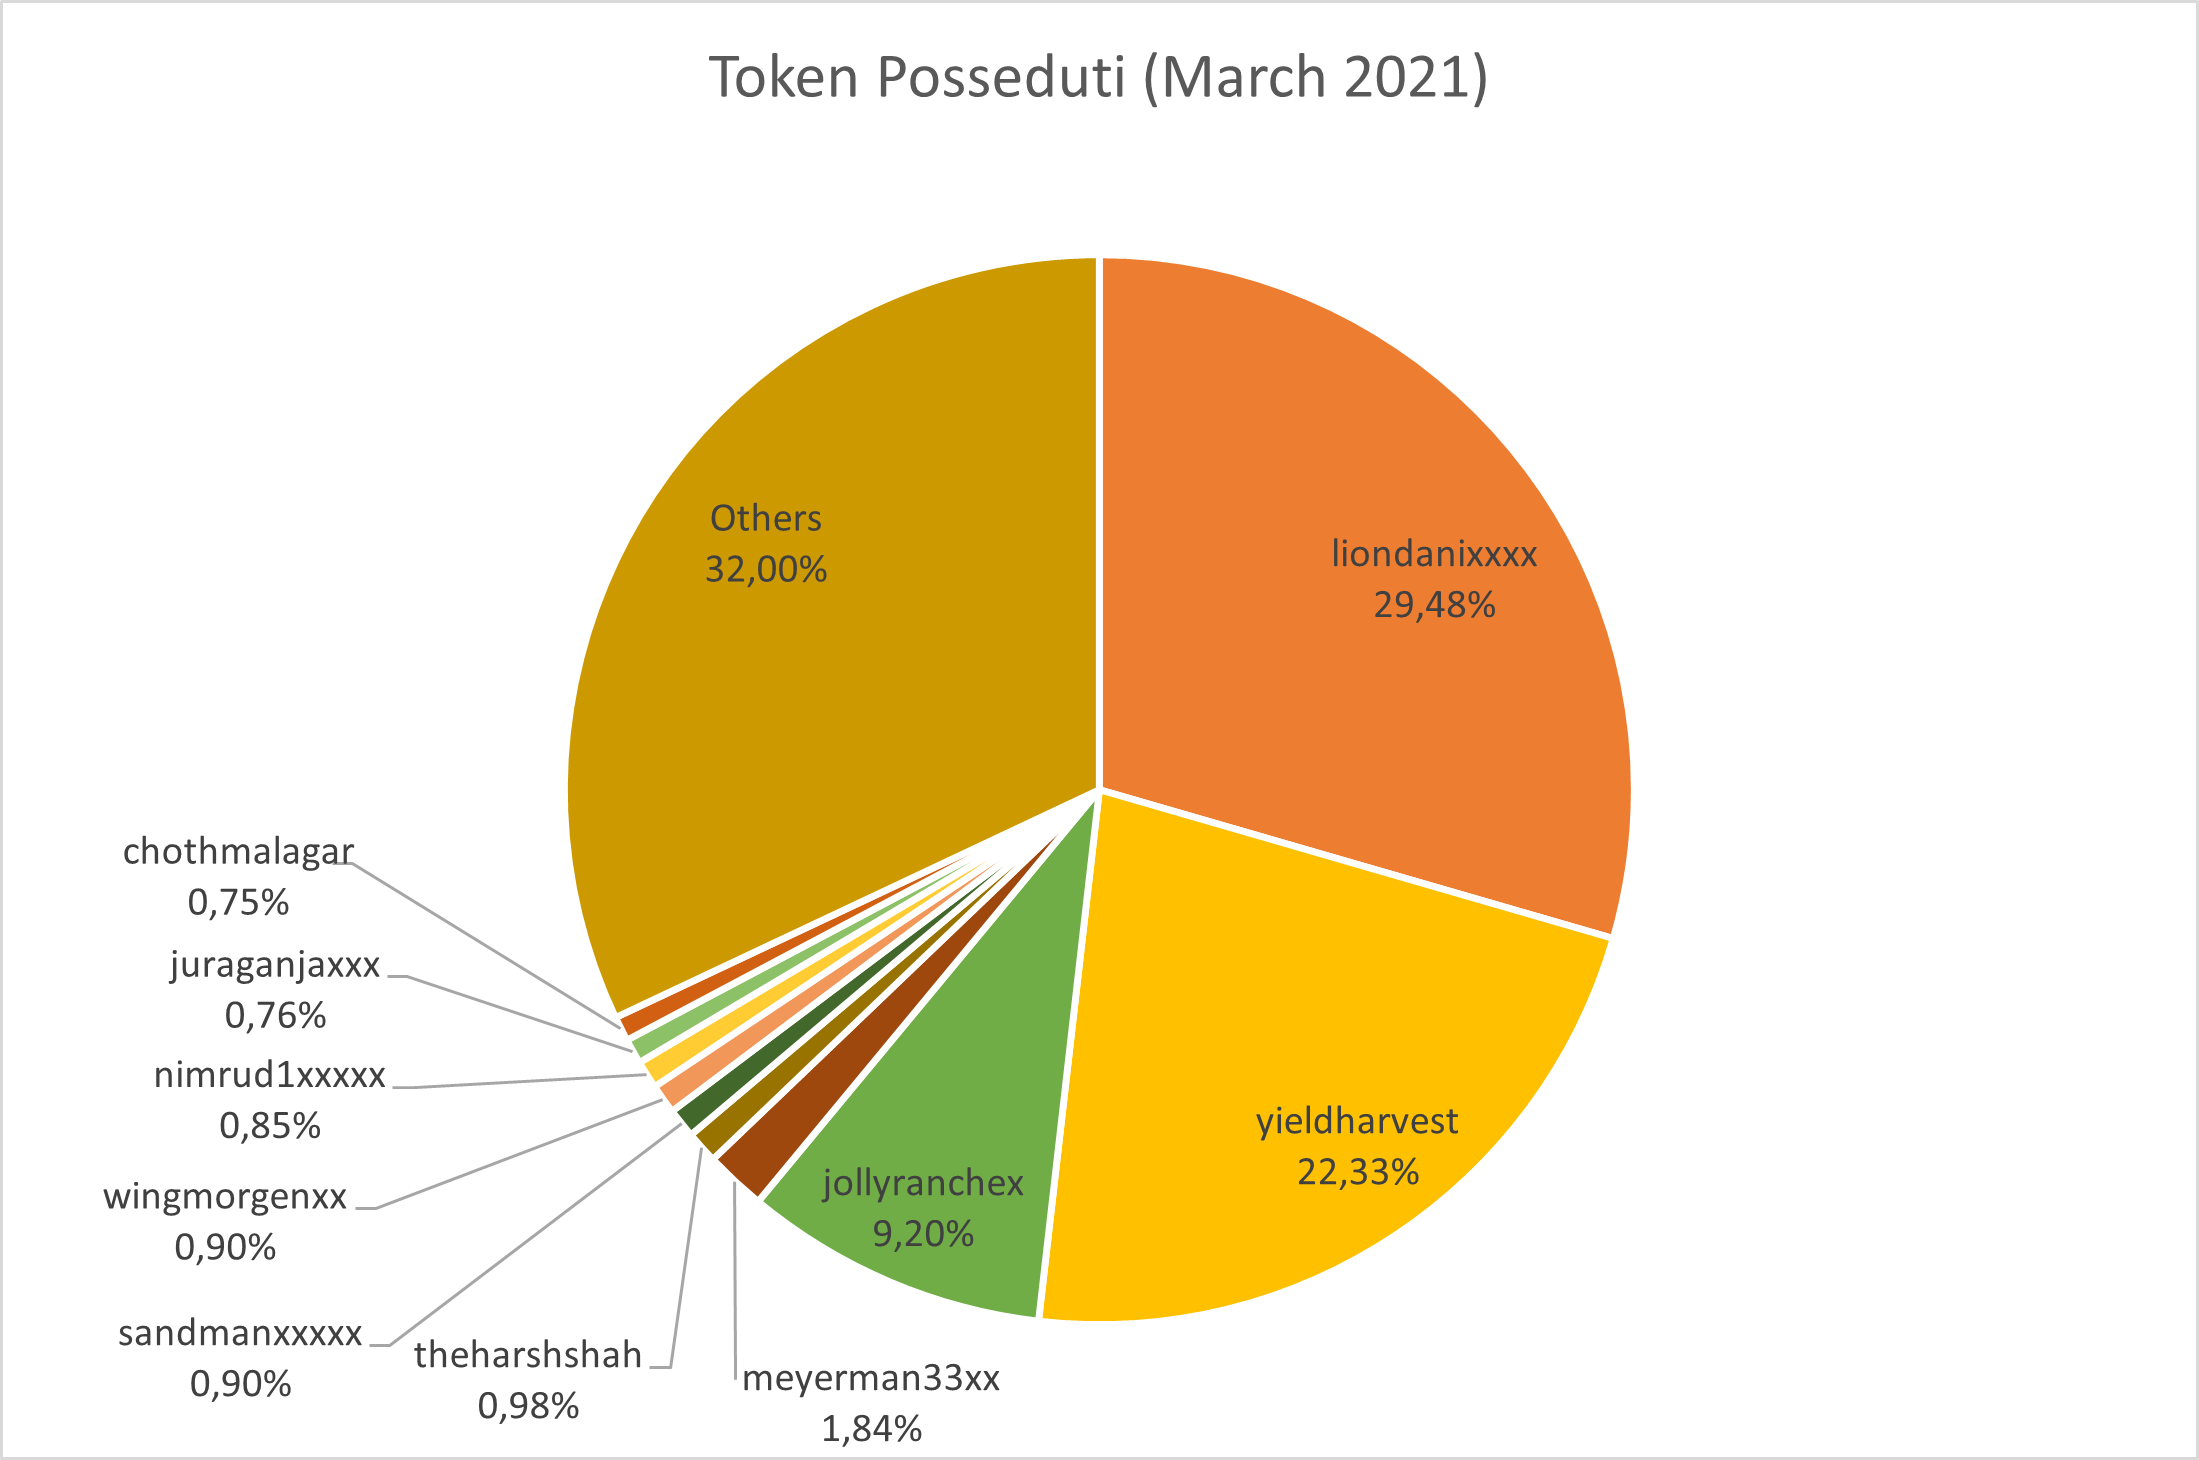
\includegraphics[width=1\textwidth]{graphs/token_posseduti_march.png}
    \caption{Top 10 degli utenti che possiedono più token a Marzo 2021. In \textbf{others} sono inclusi tutti gli utenti restanti.}
    \label{fig: tokens_hold_march}
\end{figure}

%\todo[inline]{non ho capito la differenza tra le due figure. le prime due sono tutti i dati fino a febbraio e le seconde due sono tutti i dati fino a Marzo? [EDITED: si]}

Da notare come le classifiche dei token posseduti o riscossi, indipendentemente dal fatto che si consideri il mese di Febbraio o Marzo 2021, siano dominate da utenti che, oltre ad utilizzare la piattaforma, forniscono liquidità al protocollo: \textit{liondanixxxx}, \textit{yieldharvest}, \textit{jollyranchex}, \textit{toddsmithonl}, \textit{meyerman33xx}. Questi ultimi, oltre che a detenere le prime posizioni in classifica, possiedono sostanzialmente gran parte dei token in circolazione all'interno della community, ovvero più del 57\% nel mese di Febbraio (Figura \ref{fig: tokens_hold_feb} e più del 61\% nel mese di Marzo (Figura \ref{fig: tokens_hold_march}.

Risulta rilevante anche notare che i 3 account con più claimed tokens posseggono, in percentuale, più token di quelli claimed.
Questo importante fatto ci mostra che dietro le attività di voto esiste una certa economia di scambio di monete e che alcuni utenti riescono ad arricchirsi non necessariamente solo tramite il meccanismo del voto.
Infine, confrontando i risultati ottenuti a Febbraio 2021 con quelli ottenuti a Marzo 2021, risulta chiaro, non solo che la maggior parte della ricchezza della piattaforma è gestita da un numero esiguo di utenti (i 3 utenti più ricchi gestiscono più di metà del patrimonio in circolazione), ma anche che questi 3 utenti si stiano arricchendo di più nel tempo e che quindi il divario tra i più ricchi e tutto il resto degli utenti si stia acutizzando.

\section{Analisi Giornaliera}
Come ultima analisi ci siamo concentrati su uno studio approfondito delle azioni registrate nei mesi di Agosto e Settembre 2020, non più su base mensile, ma bensì giornaliera. L'analisi è stata effettuata con lo scopo di individuare attività inusuale in determinati giorni di quei mesi in cui era stata riscontrata maggiore attività.


In Figura \ref{fig: actions_daily} possiamo osservare la distribuzione giornaliera di tutte le azioni registrate nei mesi in oggetto della nostra analisi.

\begin{figure}[t]
    \centering
    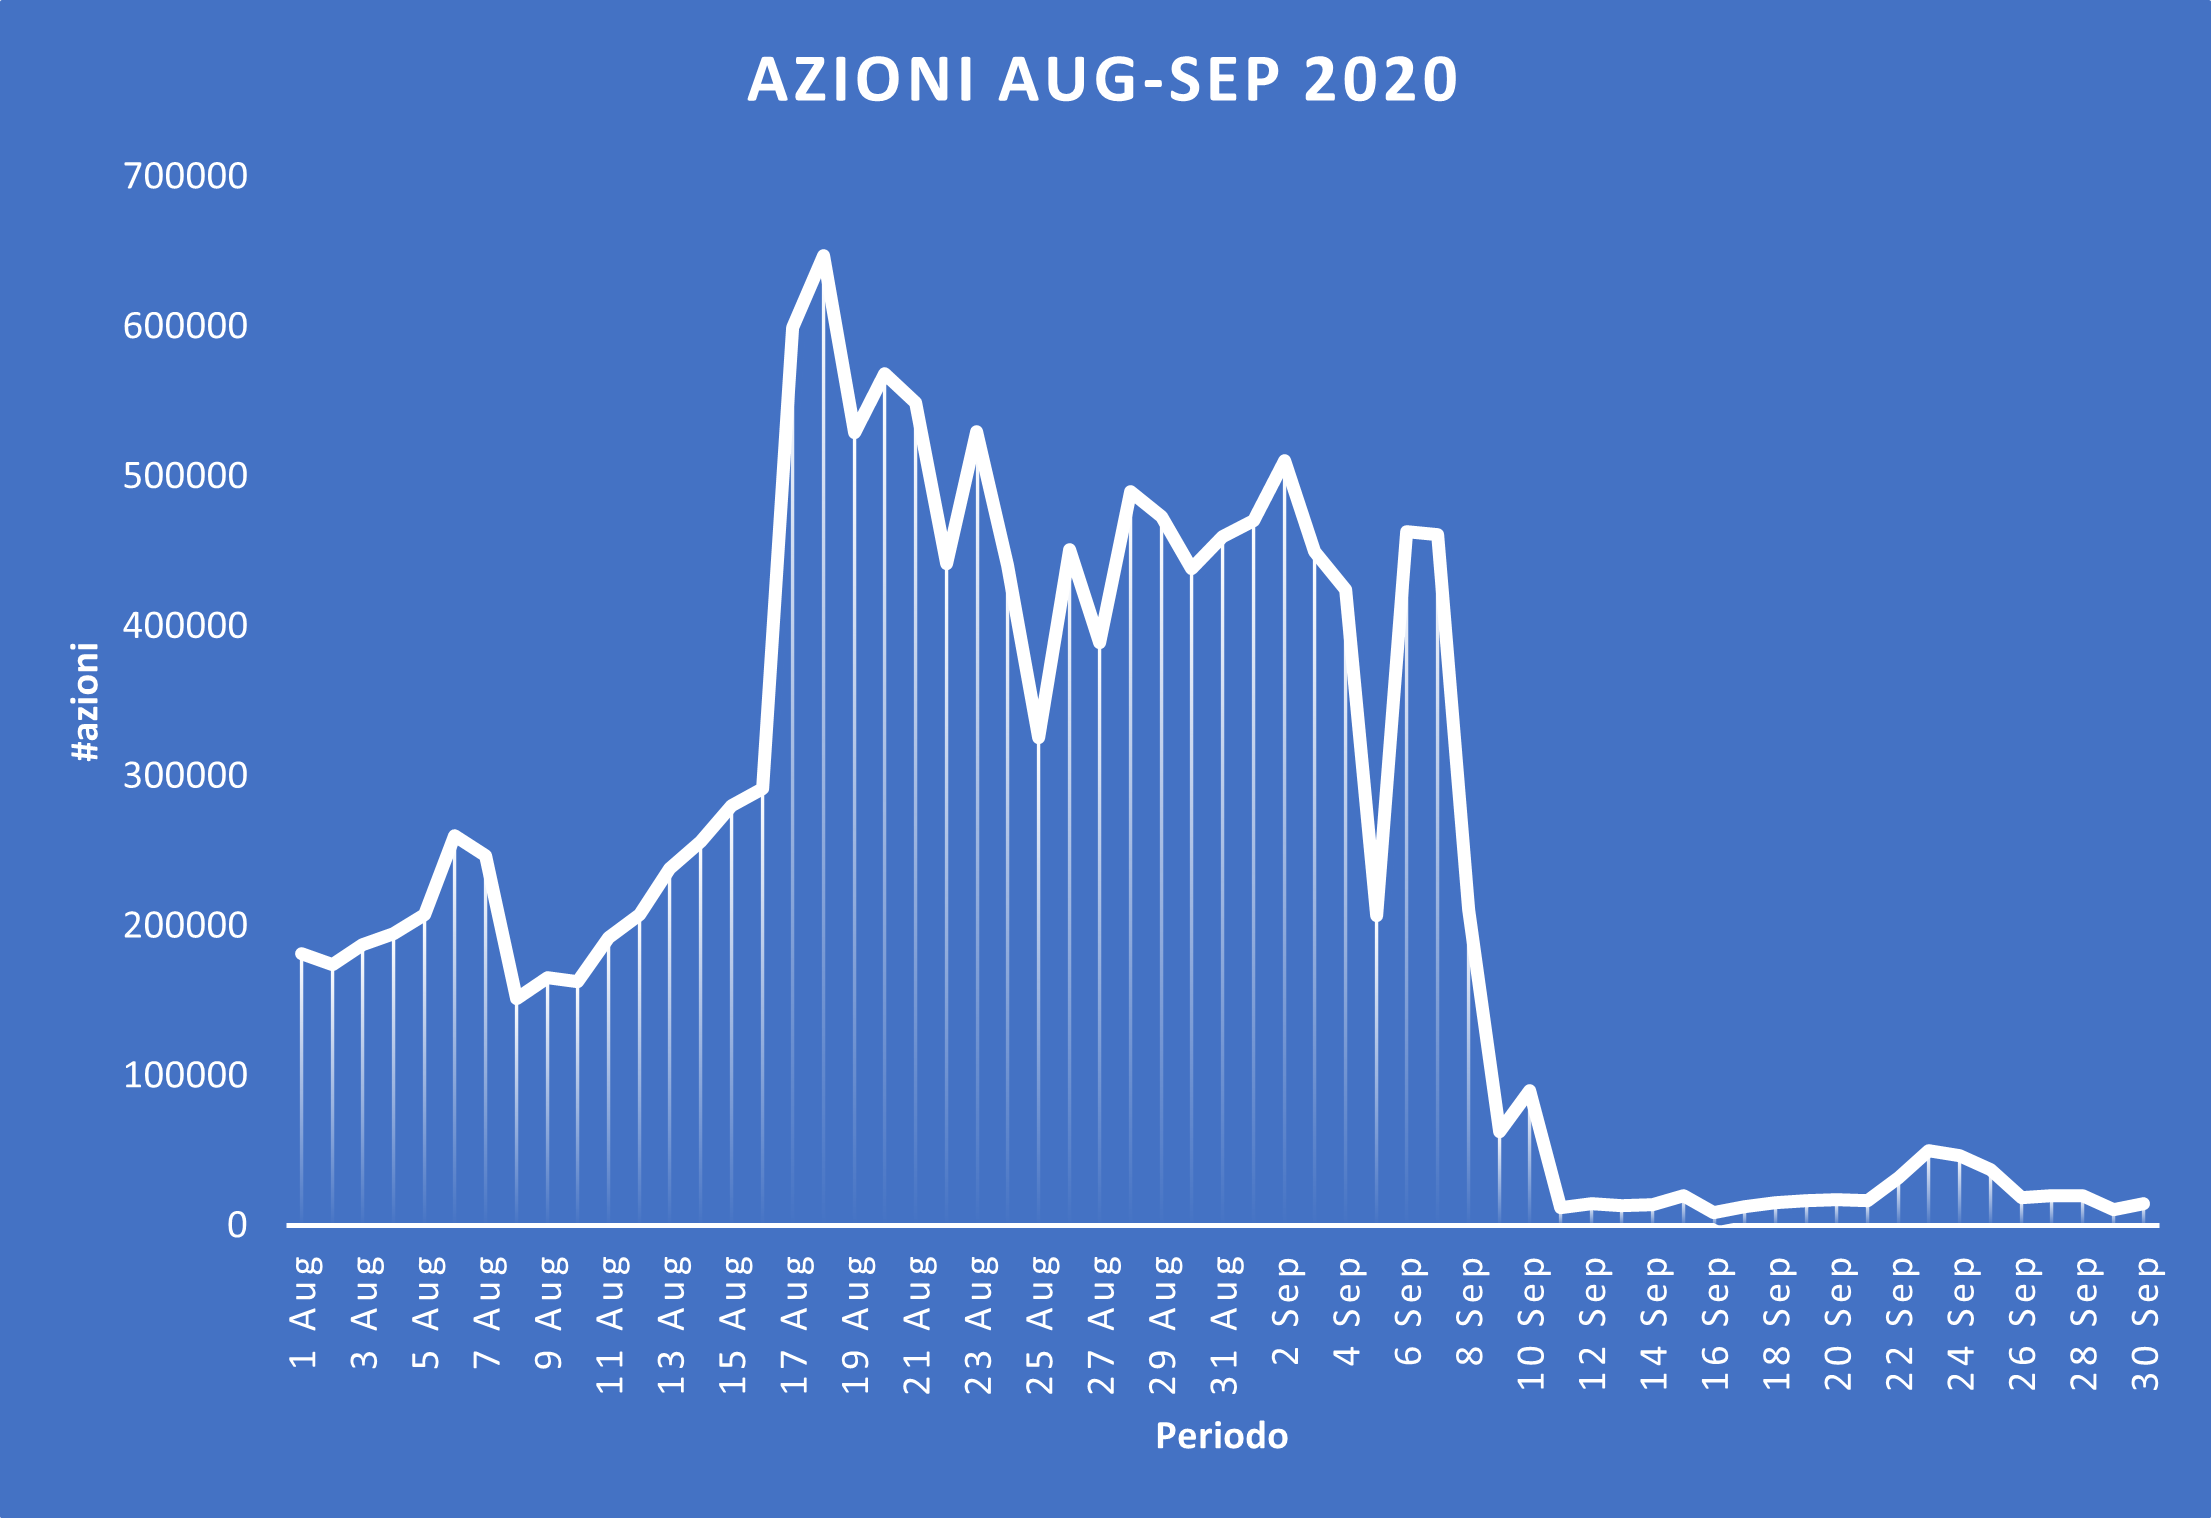
\includegraphics[width=0.8\textwidth]{graphs/daily_azioni.png}
    \caption{Distribuzione giornaliera di tutte le azioni, account Mirror inclusi.}
    \label{fig: actions_daily}
\end{figure}

La Figura ci mostra un'attività sostenuta, con circa 200.000 azioni al giorno fin dall'inizio del mese di Agosto.
L'attività su Yup si intensifica ulteriormente intorno alla metà del mese, superando le 400.000 azioni al giorno, ad eccezione di rari casi.
L'attività rimane molto alta fino all'inizio di Settembre, momento nel quale subisce un brusco arresto, fino quasi a sparire fino alla fine del mese.
Le cause di questo fenomeno non sono chiare, anche se possiamo ipotizzare che sono dovute a problemi tecnici legati alla blockchain EOS.
Infatti, come spiegato nel Capitolo \ref{chapter_background}, per poter effettuare azioni su EOS è necessario pagare un costo non trascurabile, in particolare di RAM e CPU.
Potrebbe essere accaduto che, in concomitanza con la nuova massa di utenti iscritta alla piattaforma, e l'algoritmo utilizzato per determinare la ricompensa, lo smart contract che gestisce la piattaforma non sia più stato in grado di calcolare le ricompense o di accettare voti.
Questi problemi tecnici potrebbero aver portato gli sviluppatori ad aver disabilitato alcuni account Mirror, come anche mostrato in Figura \ref{fig:attivi_conmirr}.

In Figura \ref{fig: createacct_daily_conmirr} e \ref{fig: createacct_daily_nomirr} riportiamo invece la distribuzione relativa alla creazione di account, rispettivamente considerando o meno account Mirror.

\begin{figure}[t]
    \centering
    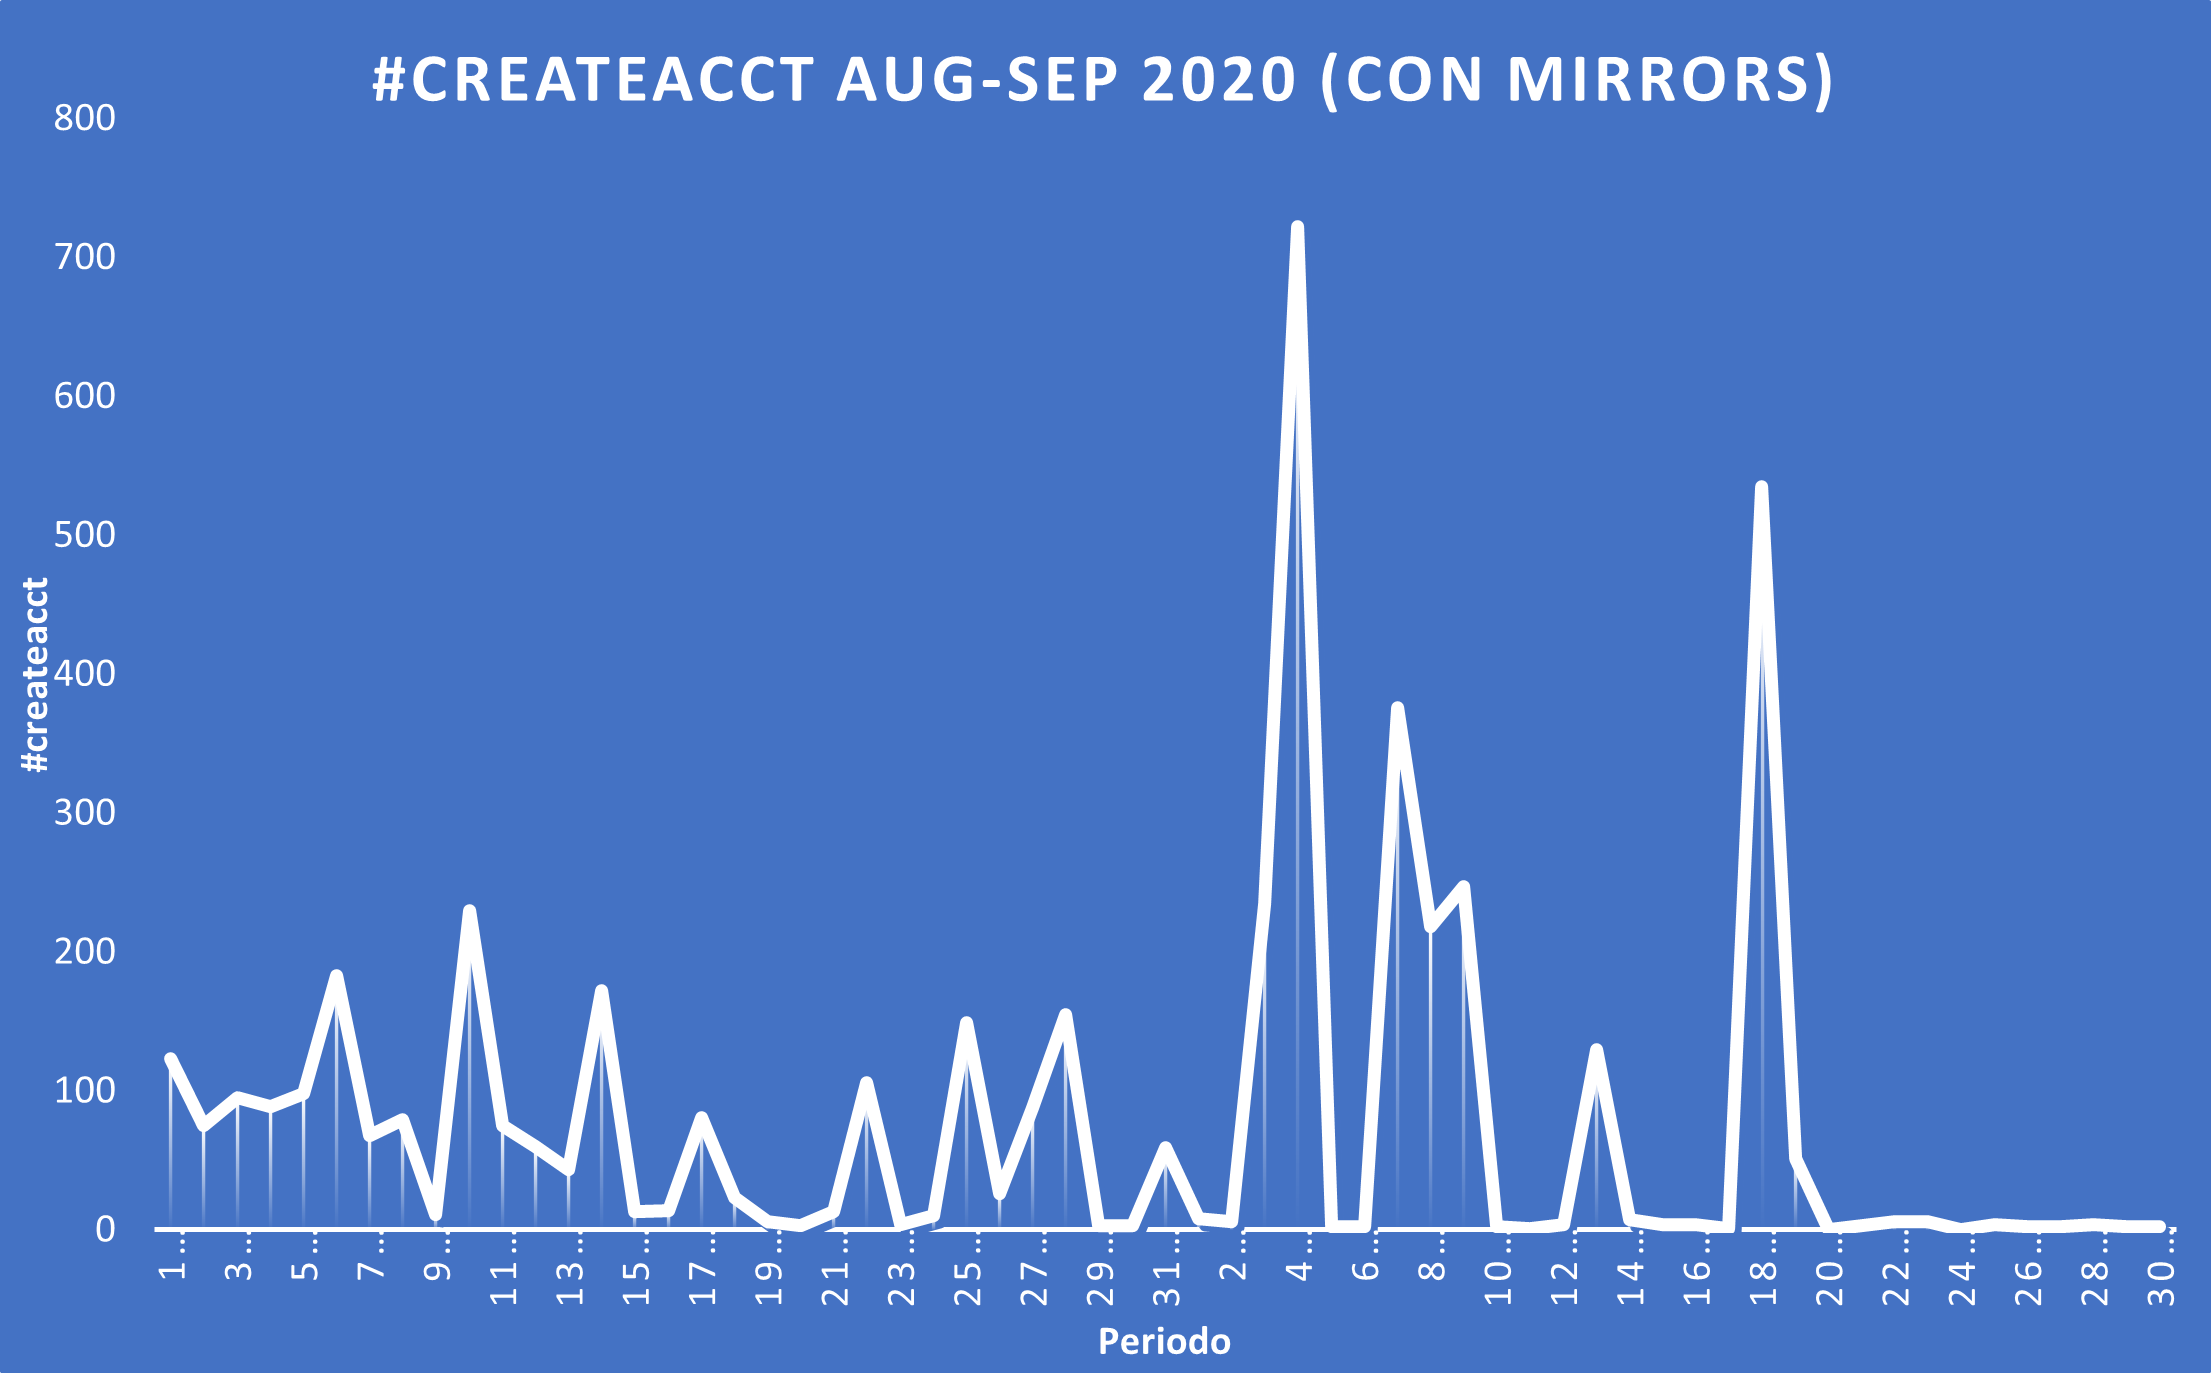
\includegraphics[width=0.8\textwidth]{graphs/daily_createacct.png}
    \caption{Distribuzione delle \textbf{createacct} su base giornaliera includendo account Mirror}
    \label{fig: createacct_daily_conmirr}
\end{figure}    
    %\vspace*{\floatstep}
\begin{figure}[t]
    \centering
    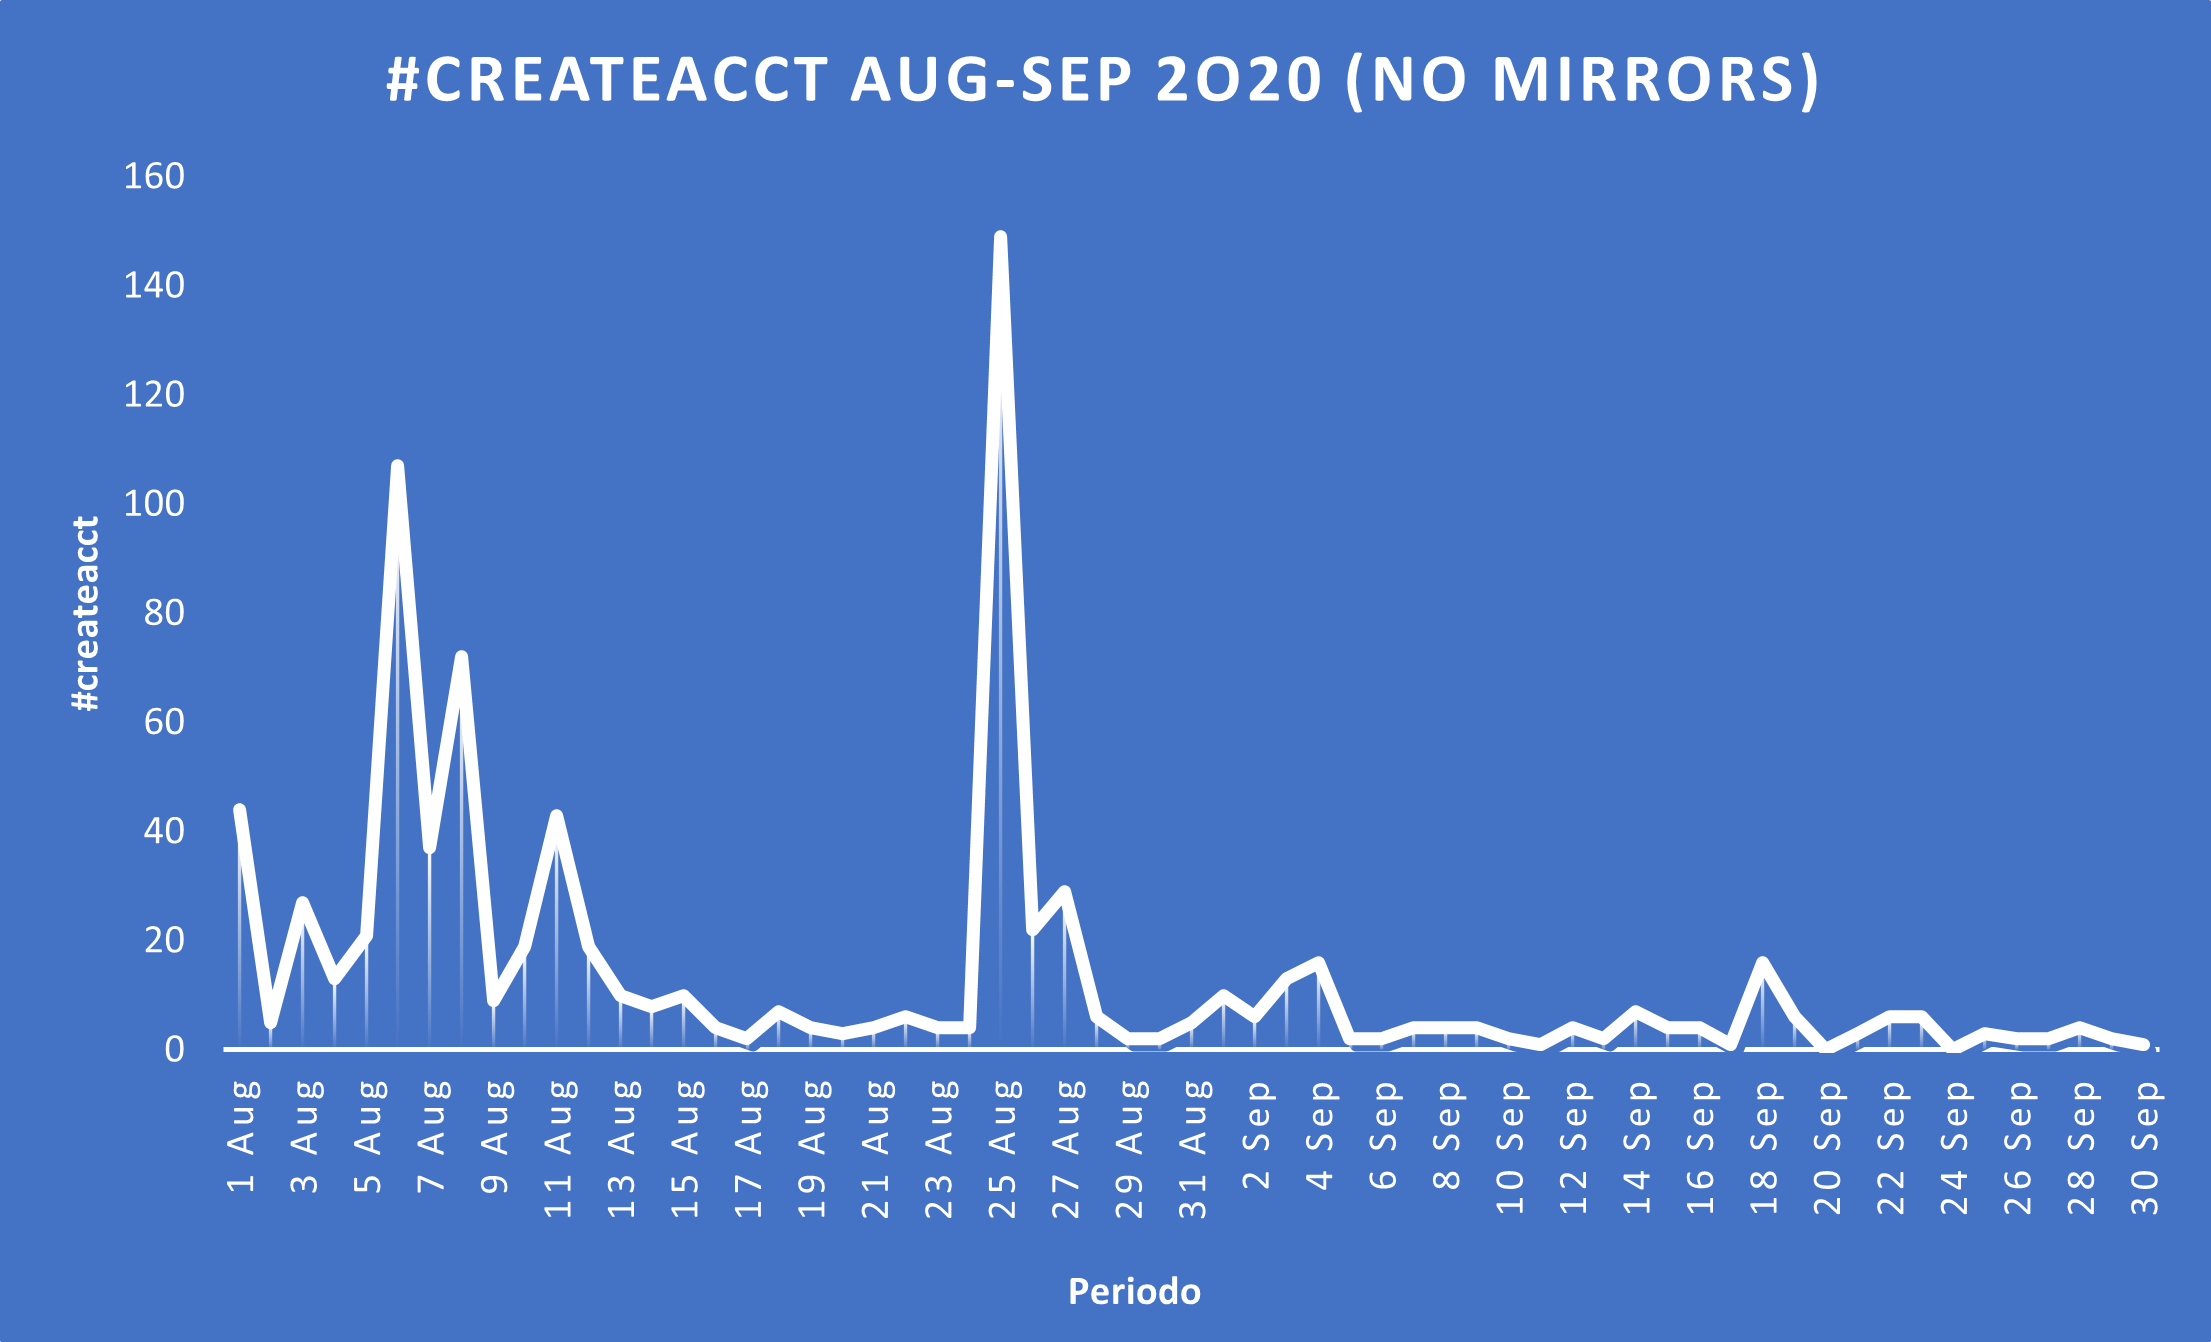
\includegraphics[width=0.8\textwidth]{graphs/daily_createacct_nomirr.png}
    \caption{Distribuzione delle \textbf{createacct} su base giornaliera escludendo account Mirror}
    \label{fig: createacct_daily_nomirr}
\end{figure}

Le Figure mostrano un andamento altalenante per quanto riguarda il numero di nuovi iscritti giornalmente.
Possiamo però notare un picco di quasi 700 nuovi account Mirror iscritti il giorno 4 Settembre e quasi 500 il giorno 18 Settembre, pochi giorni prima dei problemi tecnici ipotizzati in questa Sezione.
Siamo sicuri che siano quasi tutti Mirror perché non osserviamo picchi simili in Figura \ref{fig: createacct_daily_nomirr}.
Notiamo invece un picco di oltre 140 utenti non-Mirror iscritti il giorno 25 Agosto.

Infine i grafici su base giornaliera delle azioni di voto, Figura \ref{fig: voting_daily_conmirr} considerando tutti gli utenti, e \ref{fig: voting_daily_nomirr} senza considerare i Mirror, e degli utenti attivi, Figura \ref{fig: attivi_daily_conmirr} considerando tutti gli utenti, e \ref{fig: attivi_daily_nomirr} senza considerare i Mirror.
Abbiamo tentato di individuare qualcosa che motivasse questo picco andando a vedere se ci fossero tweet in quei giorni e in quelli antecedenti sul profilo Twitter di Yup e su quello degli influencer maggiormente votati dagli utenti (Elon Musk, Binance, ecc.), purtroppo senza successo. Il motivo di un picco del genere in quel periodo è pertanto sconosciuto.

\begin{figure}[t]
    \centering
    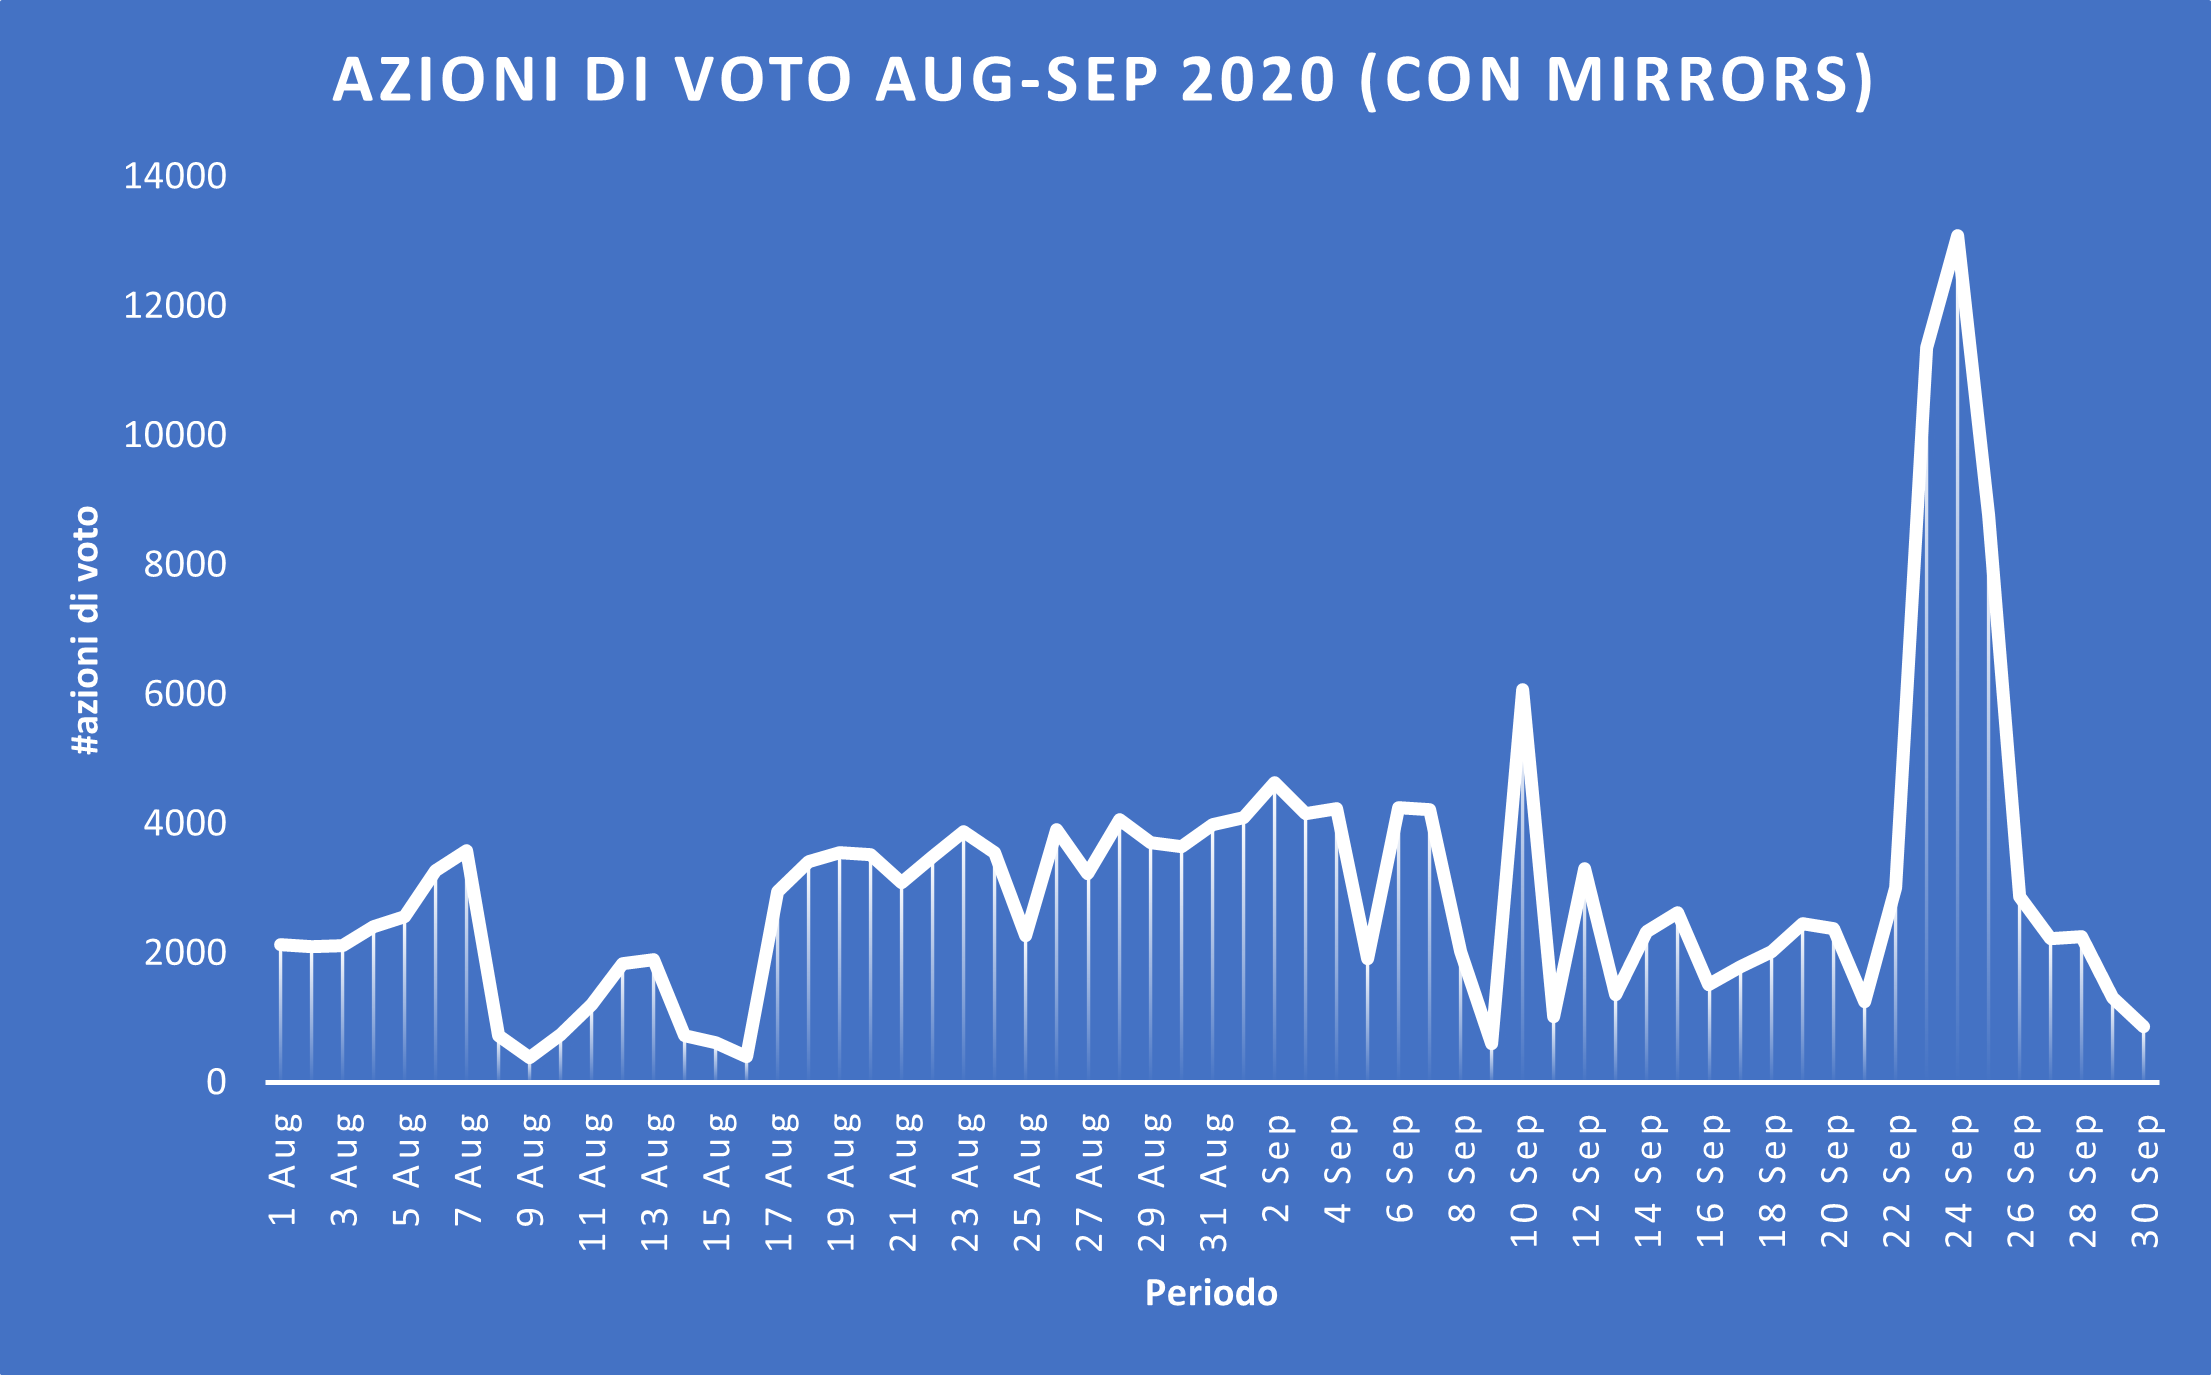
\includegraphics[width=.7\textwidth]{graphs/daily_azionivoto.png}
    \caption{Distribuzione giornaliera delle azioni di voto, incluse quelle effettuate da account mirror}
    \label{fig: voting_daily_conmirr}
\end{figure}    
    
    
\begin{figure}[t]
    \centering
    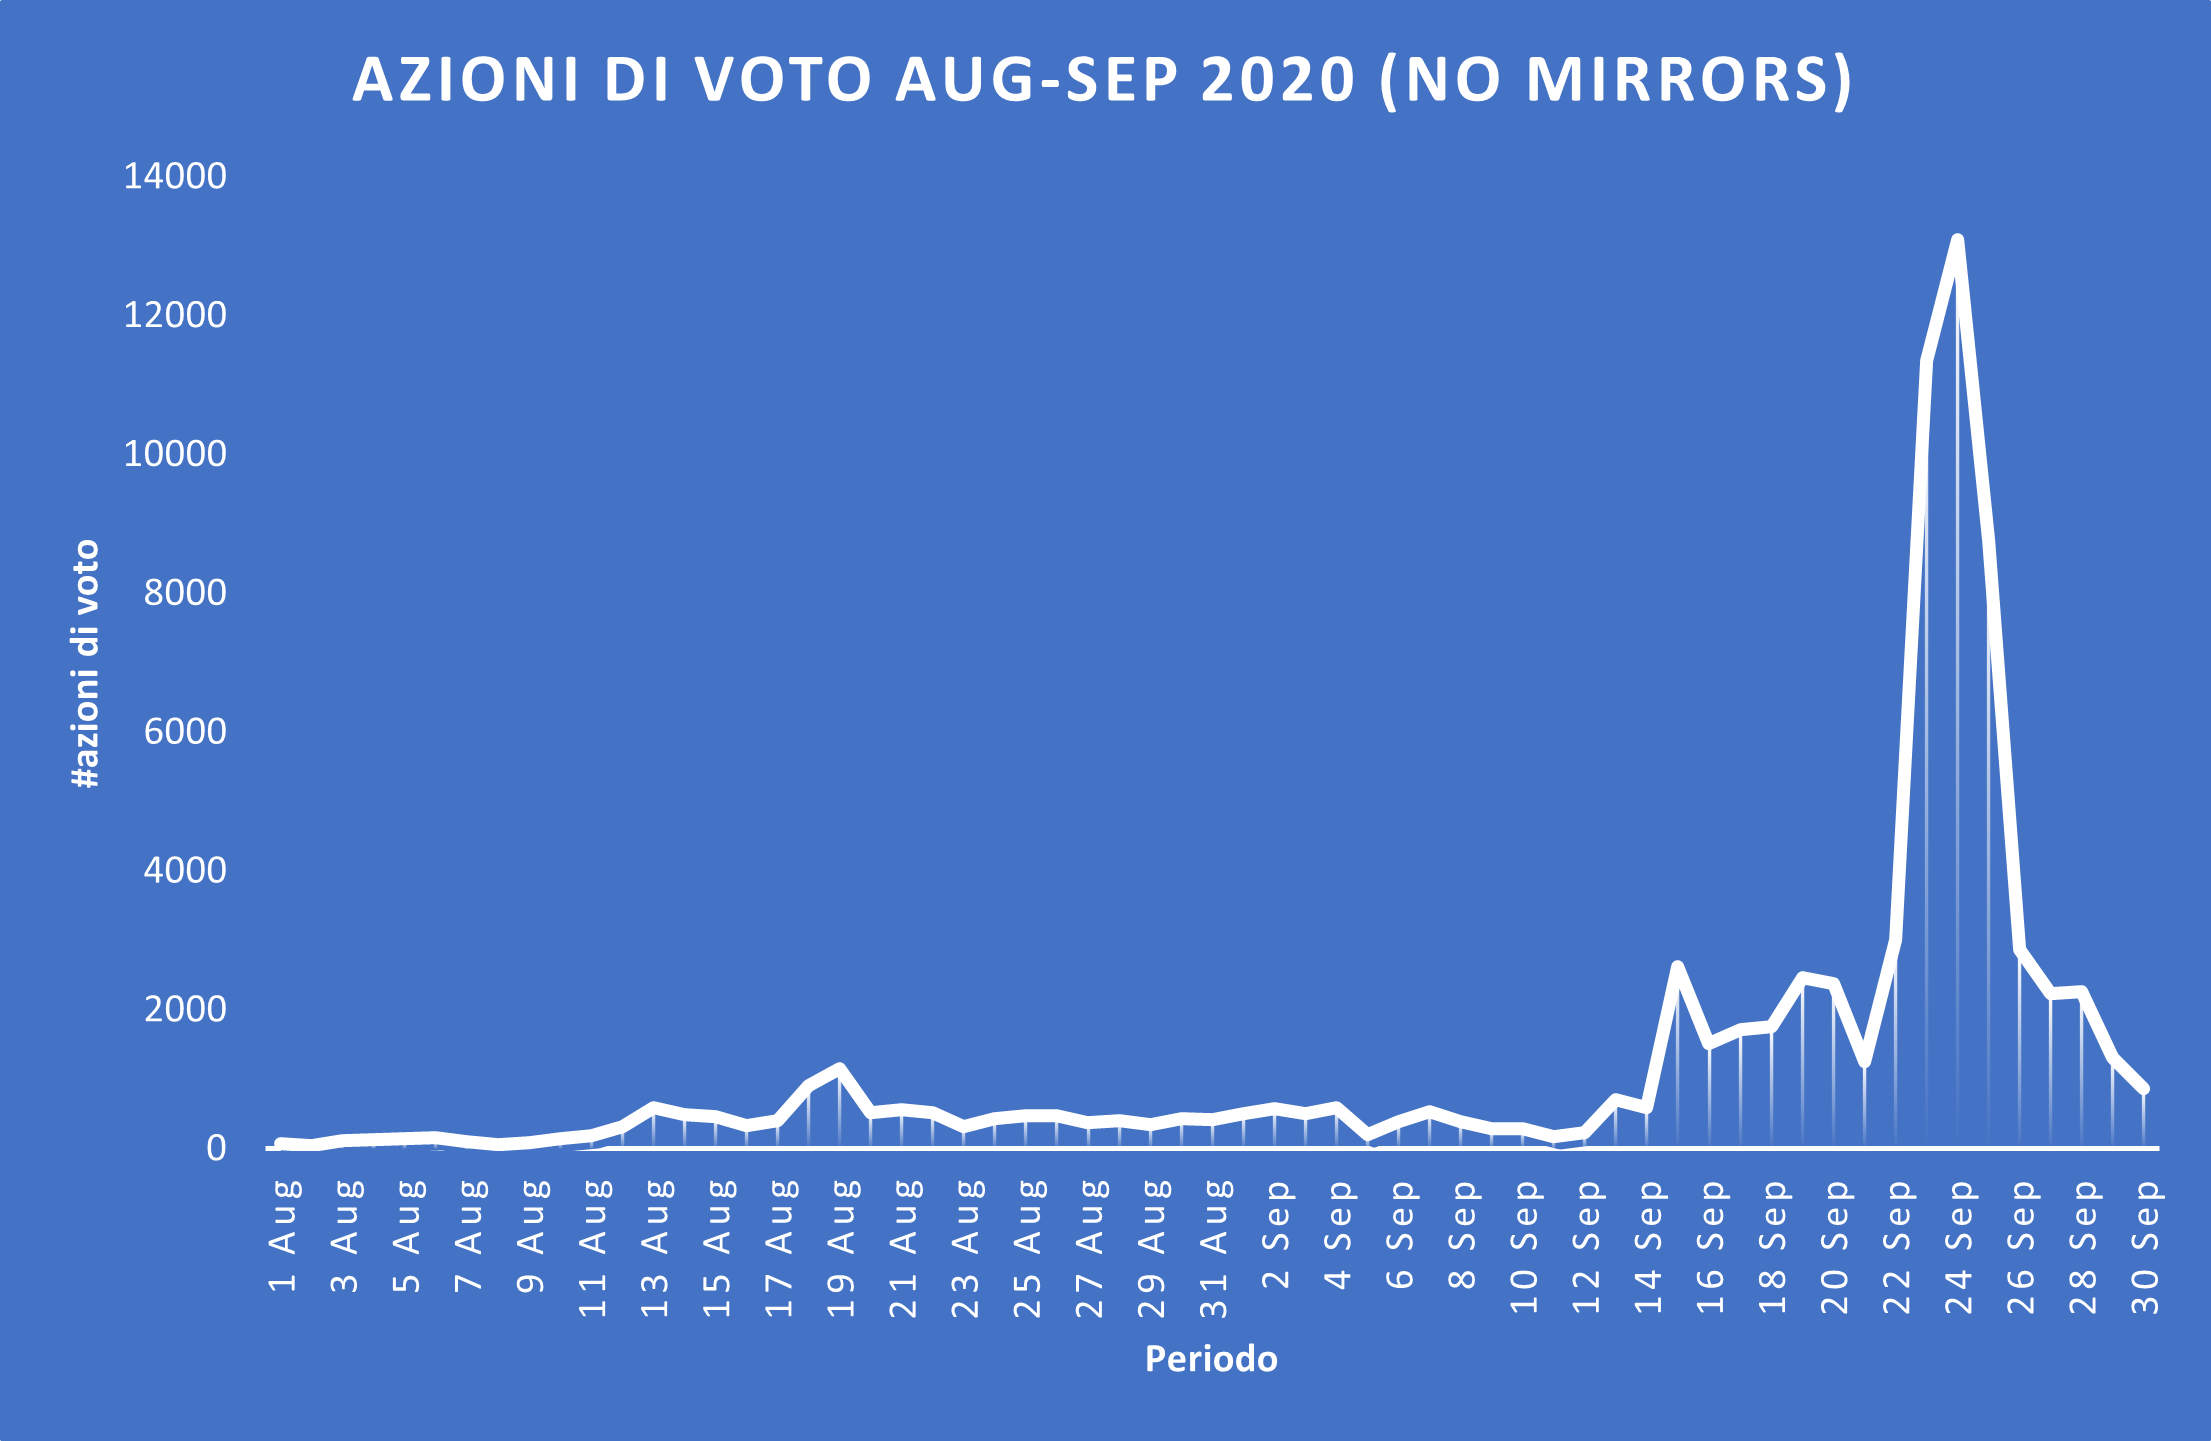
\includegraphics[width=.7\textwidth]{graphs/daily_azionivoto_nomirr.png}
    \caption{Distribuzione giornaliere delle azioni di voto, escluse quelle effettuate da account mirror}
    \label{fig: voting_daily_nomirr}
    
\end{figure}    
    %\vspace*{\floatstep}
\begin{figure}[t]
    \centering
    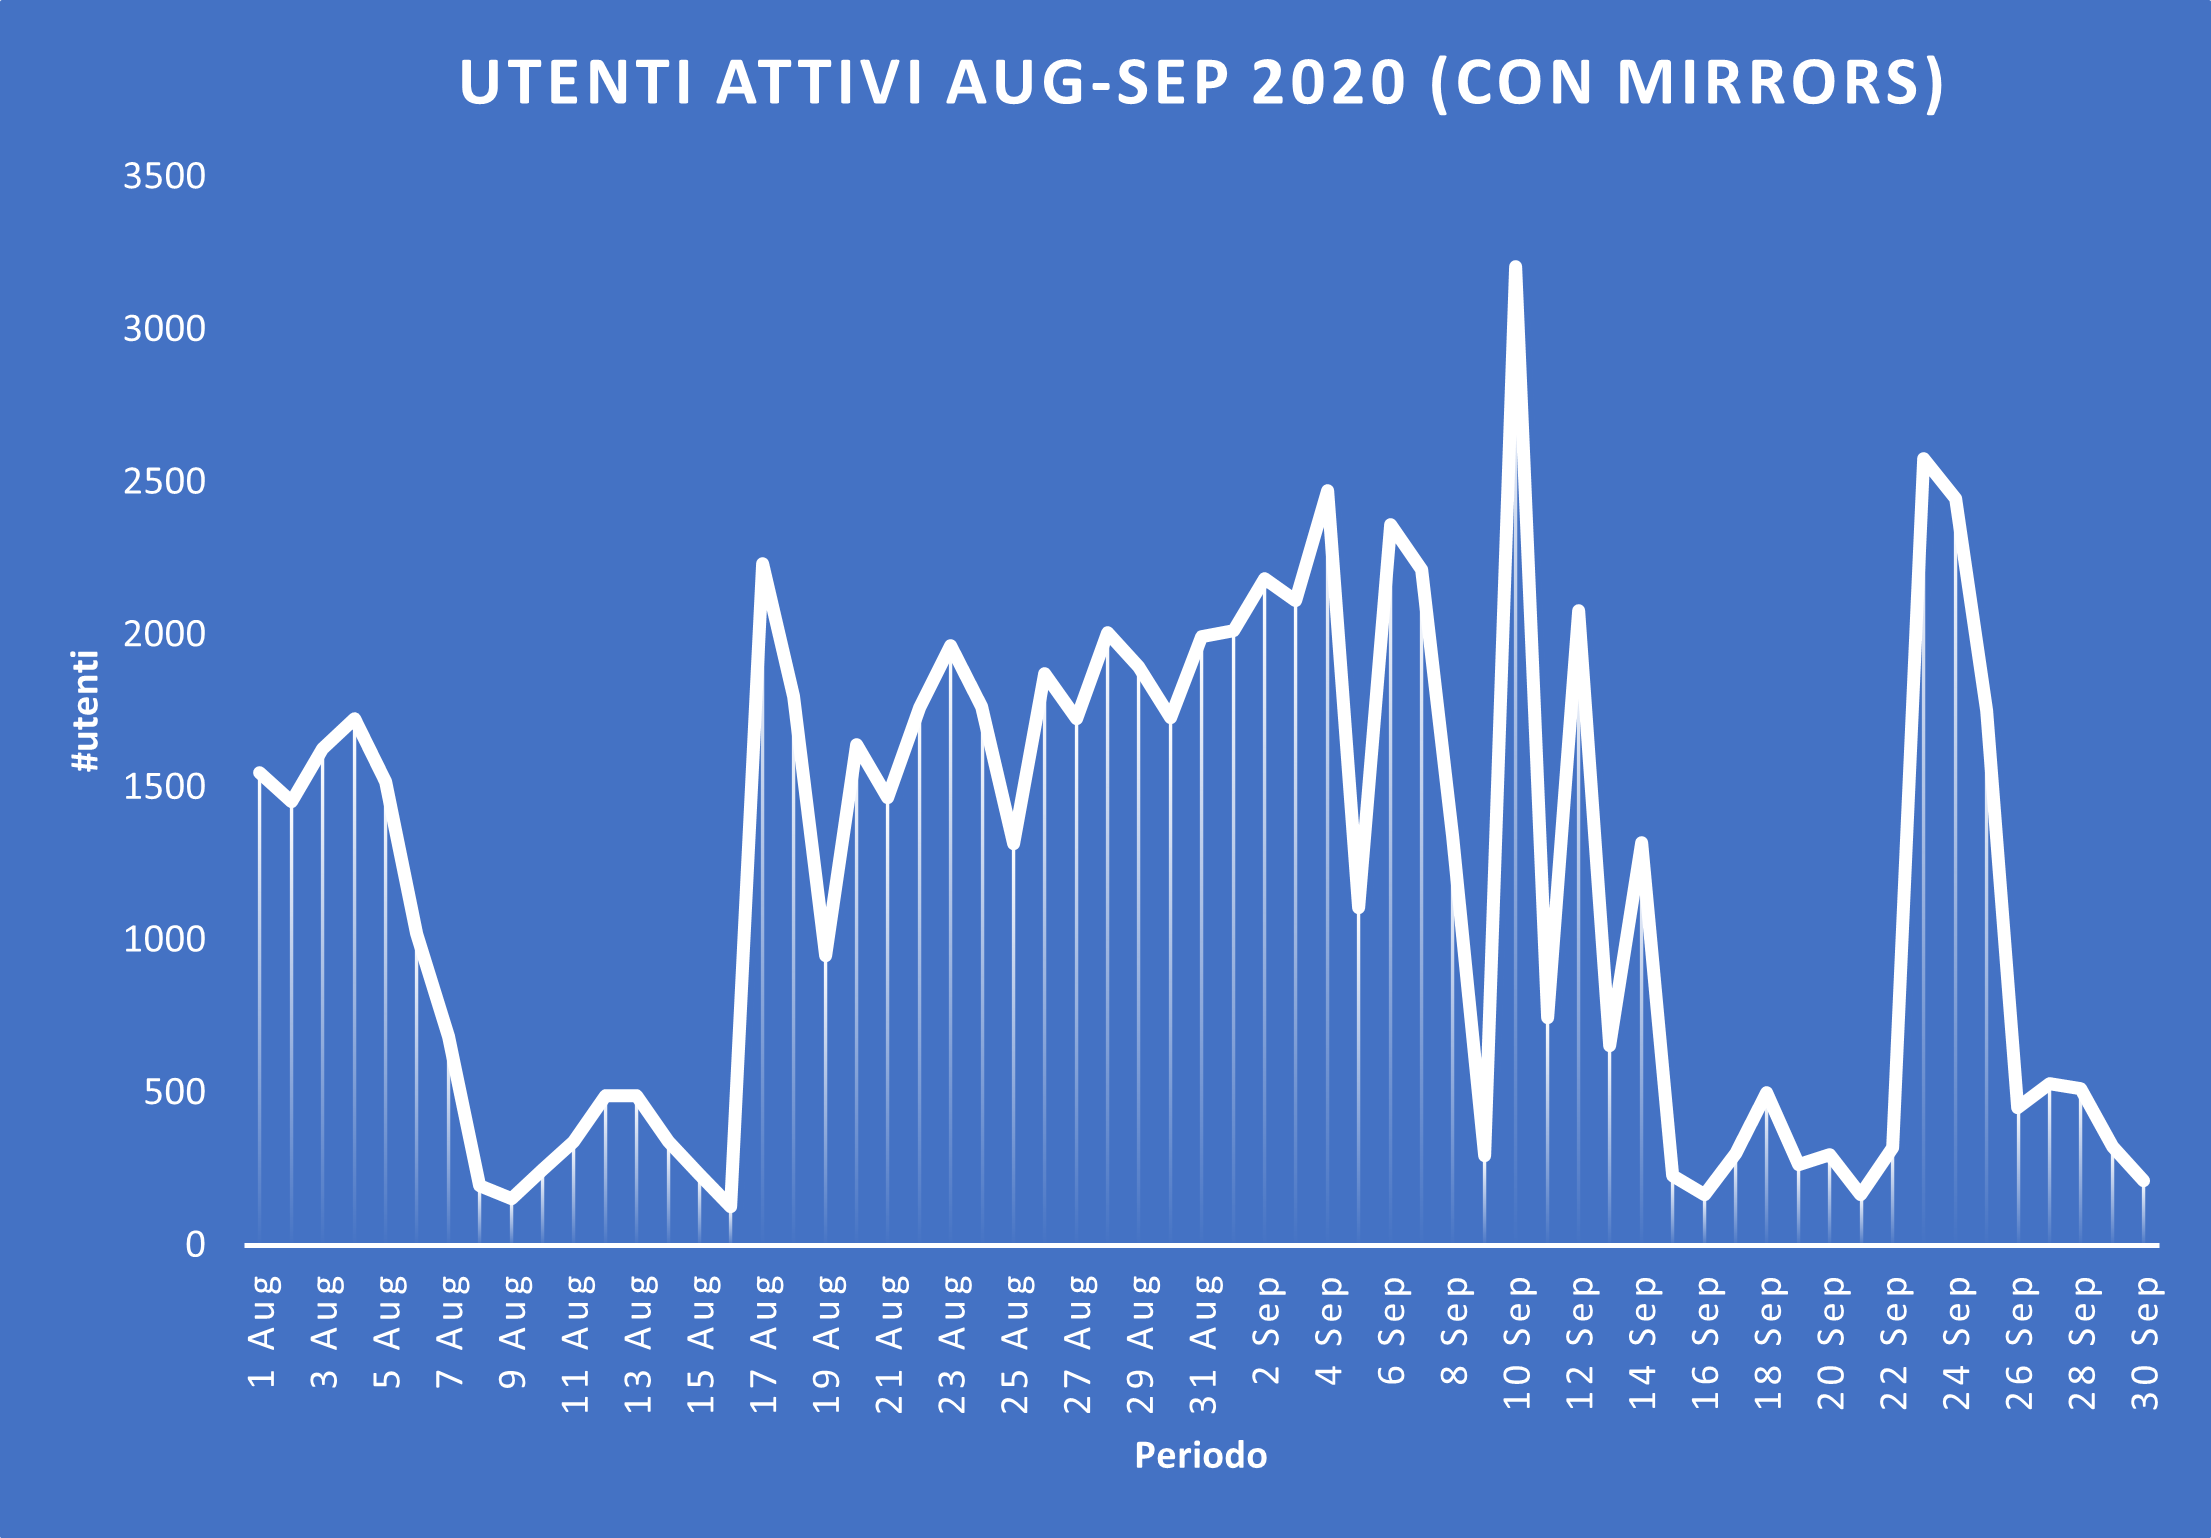
\includegraphics[width=.7\textwidth]{graphs/daily_attivi.png}
    \caption{Utenti attivi su base giornaliera includendo i Mirror}
    \label{fig: attivi_daily_conmirr}
\end{figure}


\begin{figure}[t]
    \centering
    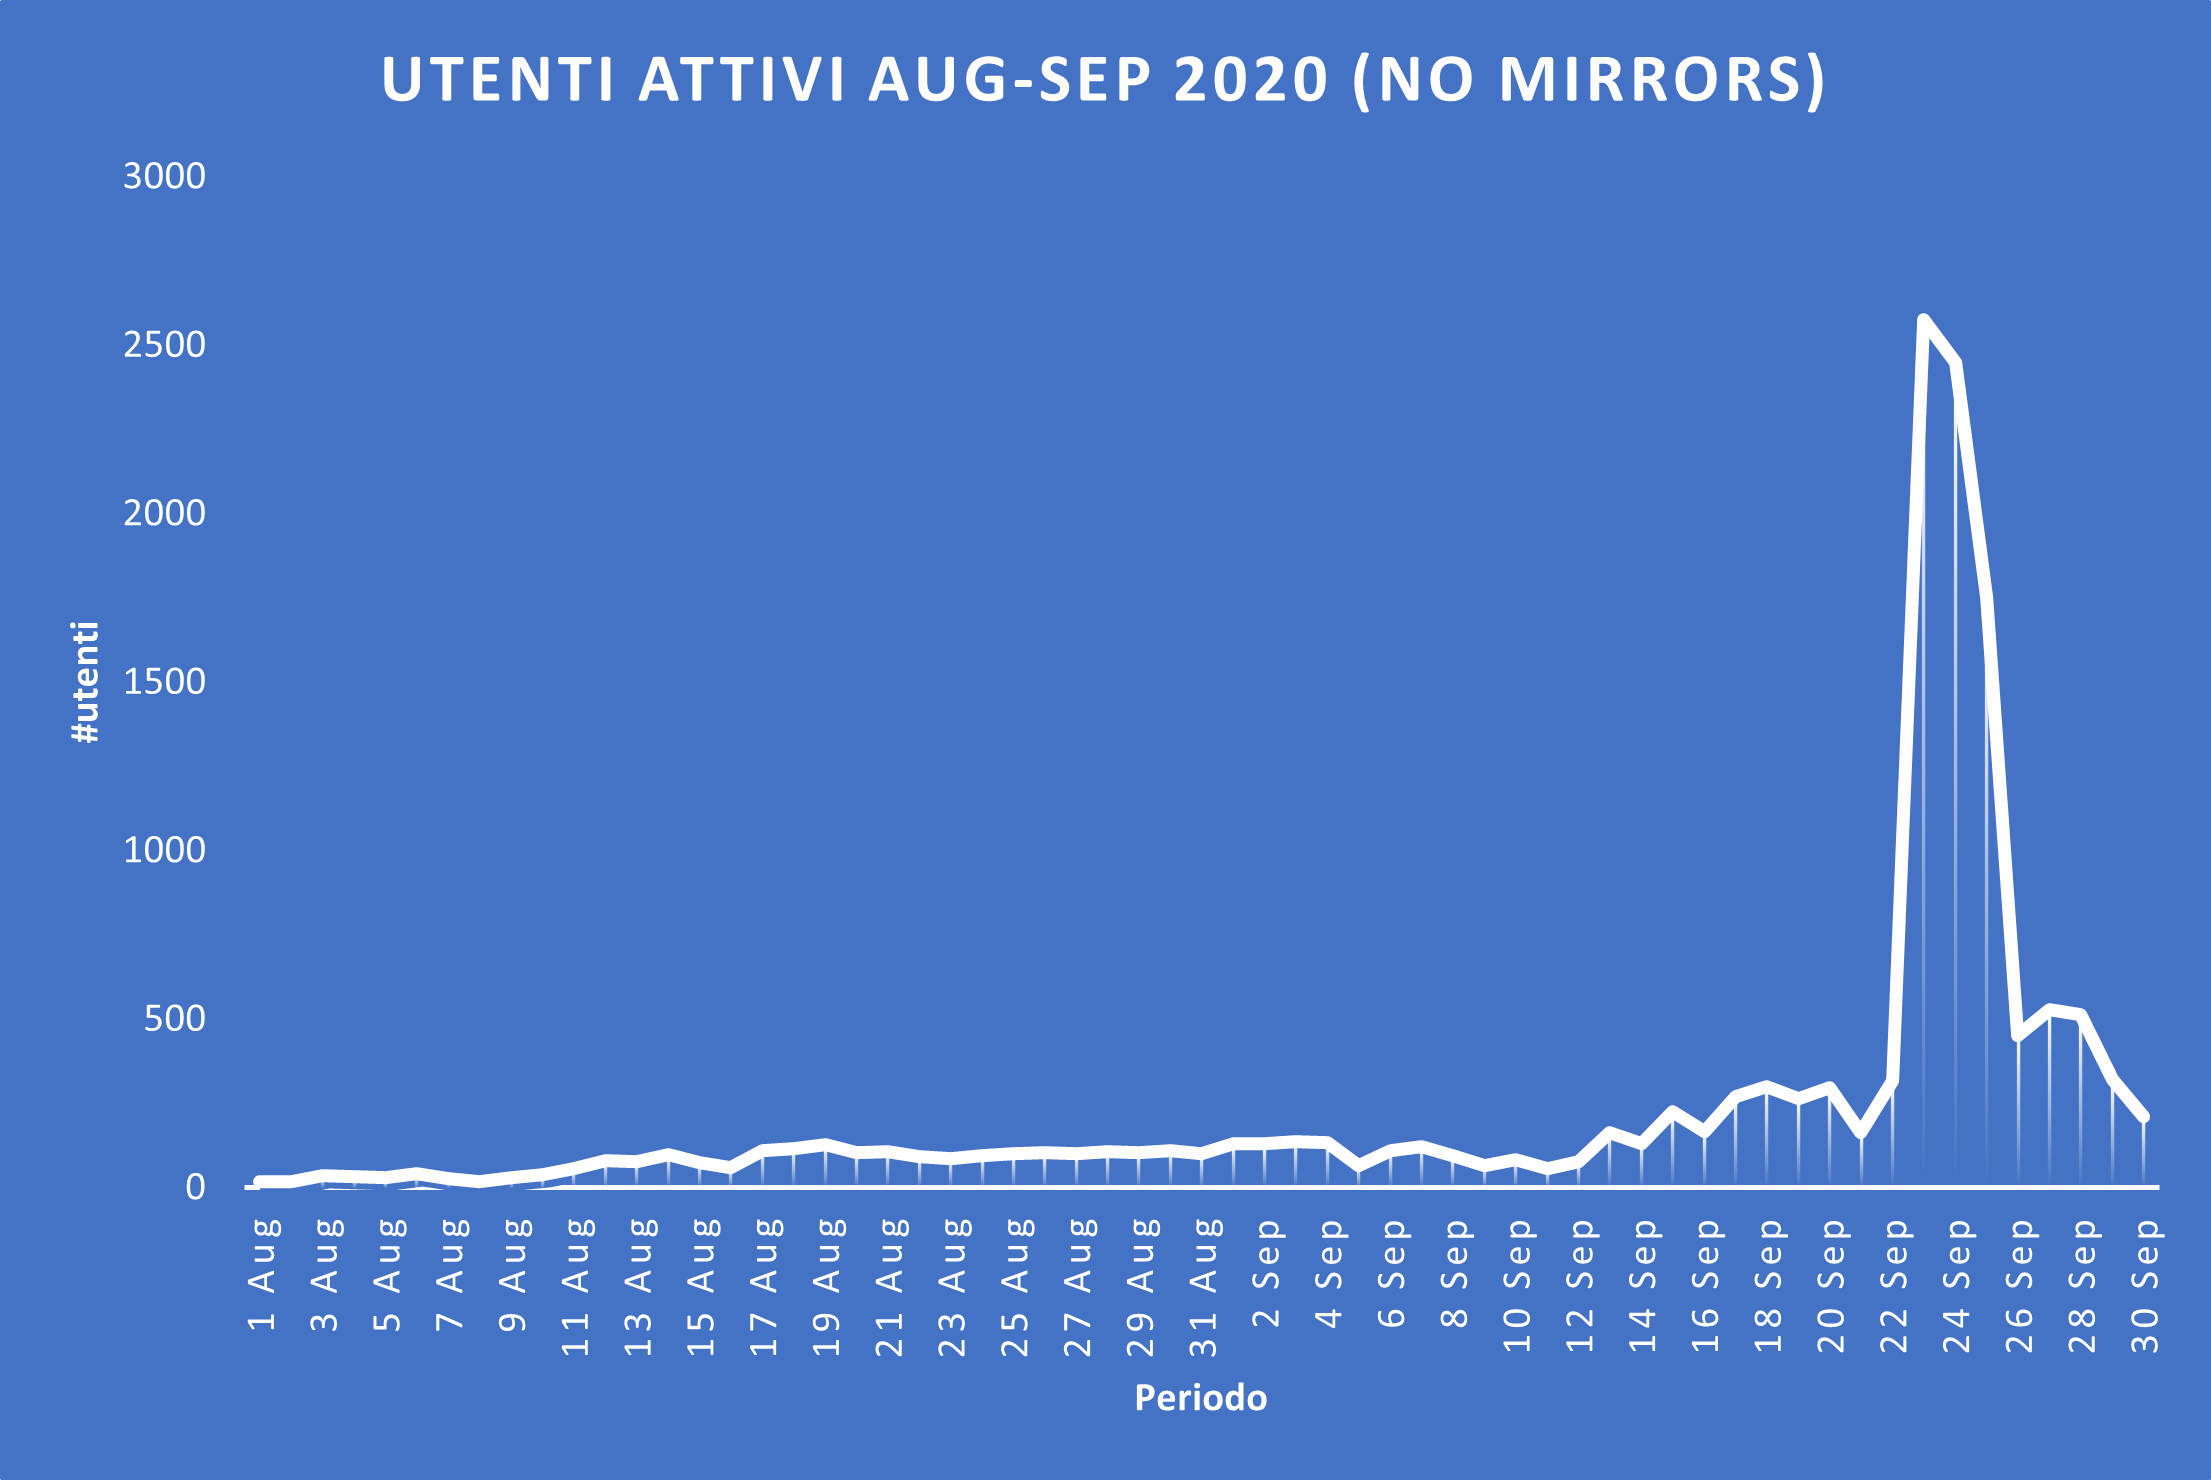
\includegraphics[width=.7\textwidth]{graphs/daily_attivi_nomirr.png}
    \caption{Utenti attivi su base giornaliera escludendo i Mirror}
    \label{fig: attivi_daily_nomirr}
\end{figure}

Si può notare un picco ricorrente, in data 23-24 Settembre 2020, in tutti e quattro gli ultimi grafici trattati e quindi indipendentemente dall'inclusione di account di sistema. Abbiamo tentato di individuare qualcosa che motivasse tale picco, purtroppo senza successo. Non sono stati individuati tweet sull'account ufficiale di Yup che promuovesse l'inizio di un qualche evento e non sono stati individuati nemmeno tweet che citassero Yup su account degli influencer maggiormente votati dalla community. Entrambe le eventualità avrebbero potuto causare l'incremento dell'attività voto. Il motivo di un picco del genere in quel periodo rimane pertanto sconosciuto.
